\documentclass[11pt]{beamer}	% Compile at least twice!
\usetheme{Warsaw}
\usepackage{style/talk}
\usepackage{style/links}

\renewcommand{\qed}{\textcolor{black}{\openbox}}
\usepackage{diagbox}
% Legendre Symbols
\newcommand{\genlegendre}[4]{%
  \genfrac{(}{)}{}{#1}{#3}{#4}%
  \if\relax\detokenize{#2}\relax\else_{\!#2}\fi
}
\newcommand{\leg}[3][]{\genlegendre{}{#1}{#2}{#3}}
\newcommand{\dleg}[3][]{\genlegendre{0}{#1}{#2}{#3}}
\newcommand{\tleg}[3][]{\genlegendre{1}{#1}{#2}{#3}}

\makeatletter
\newcommand{\pushright}[1]{\ifmeasuring@#1\else\omit\hfill$\displaystyle#1$\fi\ignorespaces}
\newcommand{\pushleft}[1]{\ifmeasuring@#1\else\omit$\displaystyle#1$\hfill\fi\ignorespaces}
\makeatother

\usepackage[normalem]{ulem}

% -------------------
% Content
% -------------------
\begin{document}

% Title Slide
{
\setbeamertemplate{background canvas}{
\tikz[remember picture,overlay]
	\node[opacity=1] at (current page.center) {
	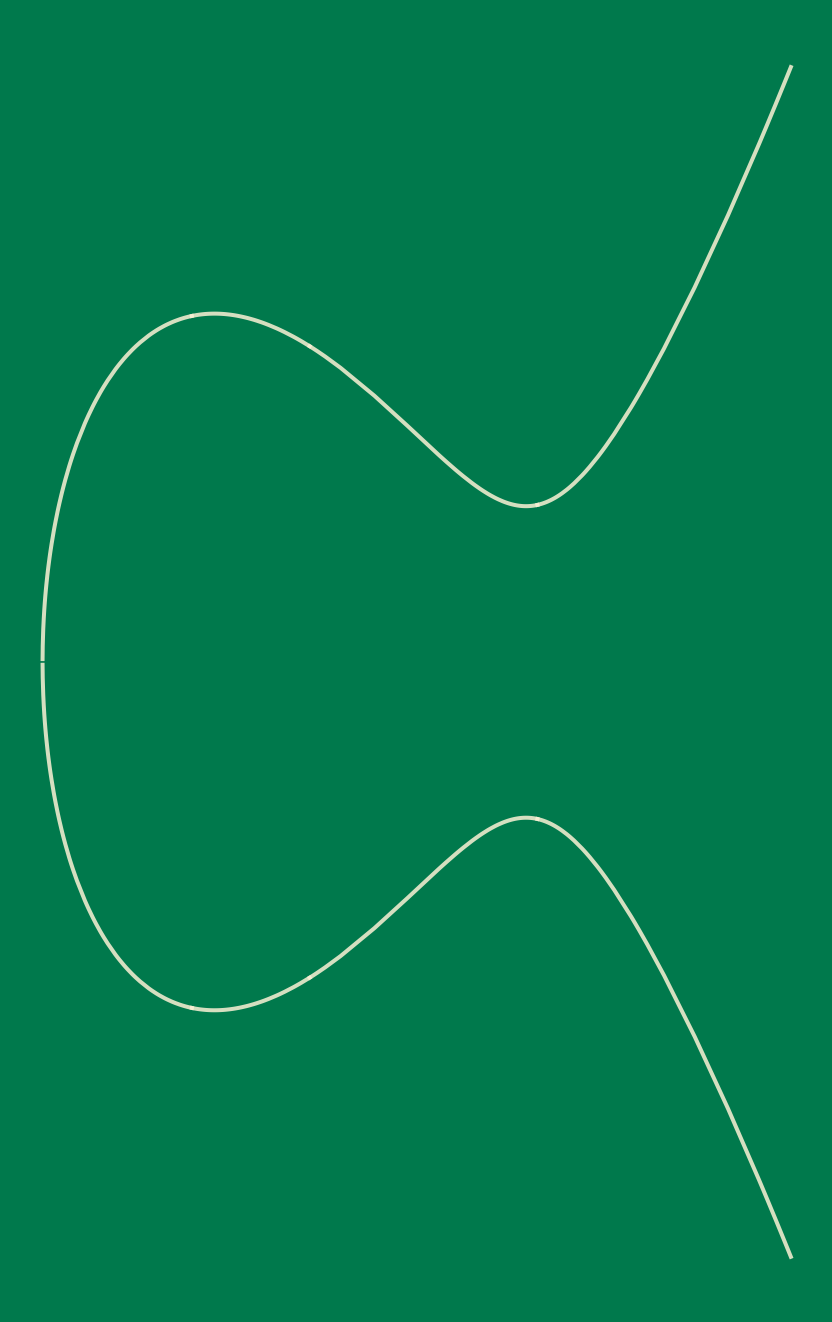
\includegraphics[width=1.05\paperwidth,
	height=\paperheight]{images/curve2.png}};} 
\begin{frame}[plain]
\phantom{.} \par\vspace{3.7cm}

% Title
\begin{center}
	{\huge\bfseries\color{egold} \textsc{Elliptic Tales:}} \par
	 {\large\bfseries\color{egold} \textsc{A Story of Bitcoin, Moonshine,}} \par
	  {\large\bfseries\color{egold} \textsc{String Theory, and Clocks}} 
\end{center} \vspace{1.5cm} 

% Author
\begin{center}
	{\bfseries\large\color{egold}\textit{Dr. Caleb McWhorter} \par
	\bfseries\textit{University of South Carolina}} \par\vspace{0cm}
\end{center} 

% Date
\begin{center}
	{\bfseries\small\color{Topazolite} March 14, 2025}
	\end{center} 
\end{frame}
}



% Introduction
% !TEX root = ../swarthmore_talk.tex

% What is Arithmetic Geometry?
\begin{frame}[plain]
\ctext{What is Arithmetic Geometry?}
\end{frame}



% Arithmetic Geometry
\begin{frame}[plain] \frametitle{Arithmetic Geometry $\approx$ Diophantine Equations}
{\scriptsize Arithmetic Geometry is approximately the study of Diophantine equations. These are named after Diophantus of Alexandria (born $\approx$ A.D.~200), who wrote a thirteen volume set called the \textit{Arithmetica} of which six survive.}

\begin{dfn}[Diophantine Equation] \scriptsize
A Diophantine equation is a polynomial equation $f(x_1, x_2, \ldots, x_n)= 0$ with integer coefficients. One may consider the coefficients to come from other rings. 
\end{dfn}

\begin{minipage}{0.5\textwidth}
	\begin{figure}[ht]
	\centering
	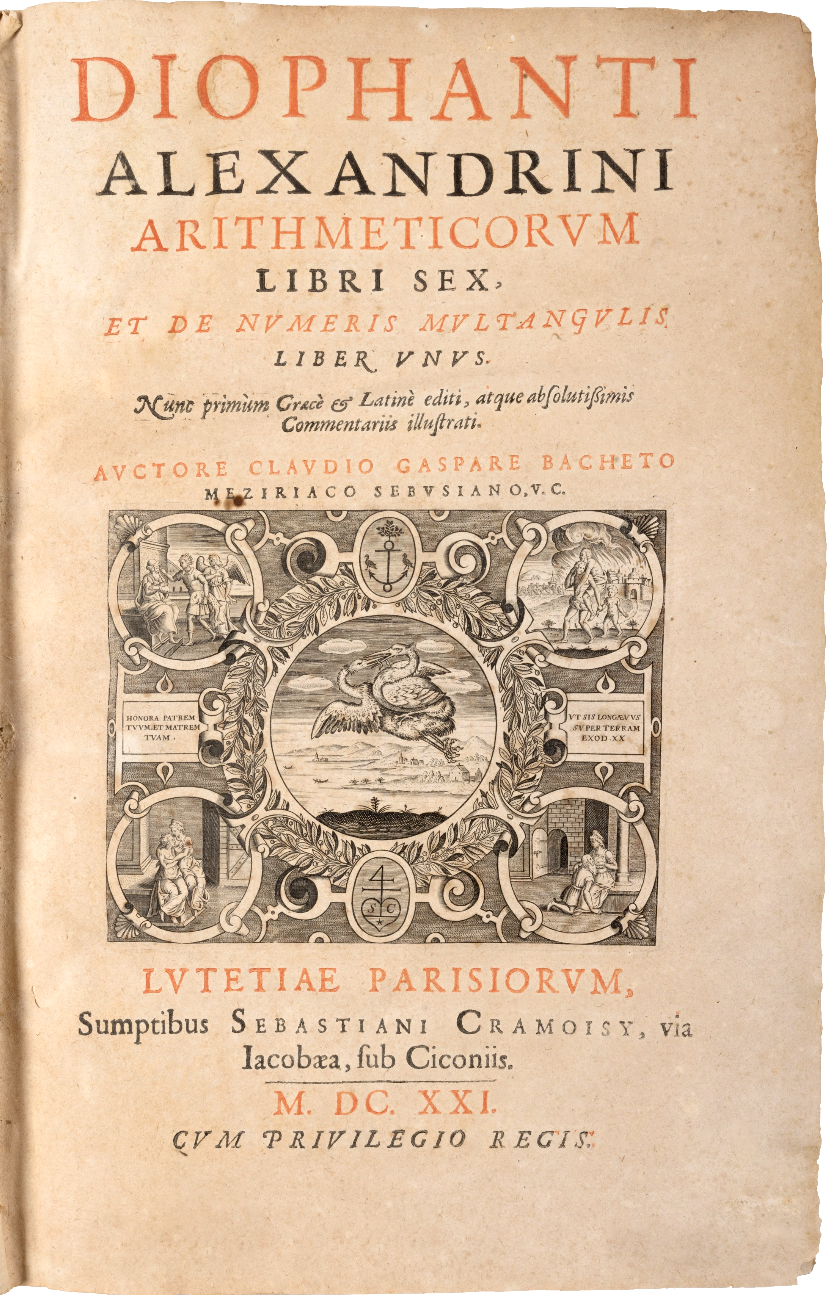
\includegraphics[width=0.6\textwidth]{images/diophantus.png}
	\end{figure}
\end{minipage}\begin{minipage}{0.55\textwidth} \scriptsize
We can ask number of questions:
	\begin{itemize}
	\item Can we determine if there are integer, rational, etc. solutions?
	\item If there are solutions, can we determine if there finitely or infinitely many?
	\item Can we find such solutions?
	\item Can we describe all the solutions?
	\item Is there an algorithm to do this generally?
	\end{itemize}
\end{minipage}
\end{frame}



% Polynomial Equations in One Variable
\begin{frame}[plain] \frametitle{Polynomial Equations in One Variable}
\small Consider the equation $f(x)= 0$, where $f(x)$ is a polynomial. \par\vspace{0.3cm}

{\itshape \bfseries Question:} Can we determine if there are `nice' solutions to a polynomial equation and, if so, determine what those solutions are? \par\vspace{0.3cm}

\begin{ex}
	\begin{itemize}
	\item $2x + 1= 5 \phantom{xxx..xx} \Longrightarrow \phantom{xxxx} x= 2$ \hfill 1 `nice' solution
	\item $x^2= 6 - x \phantom{xxx.xxx} \Longrightarrow \phantom{xxxx} x= -3, 2$ \hfill 2 `nice' solutions
	\item $x^2 - 2x - 4 = 0 \phantom{xx} \Longrightarrow \phantom{xxxx} x= 1 \pm \sqrt{5}$ \hfill 2 `not nice' solutions
	\item $x^2 + 1= 0 \phantom{xxx..xx} \Longrightarrow \phantom{xxxx.} x= \pm i$ \hfill No solutions?
	\end{itemize}
\end{ex} \par\vspace{0.3cm}
\end{frame}



% One Variable Polynomials
\begin{frame}[plain] \frametitle{The Case of One Variable Polynomials}
The case of one variable is finding the roots of a polynomial $f(x)= a_n x^n + a_{n-1} x^{n-1} + \cdots + a_0$.

\begin{thm}[Rational Roots Theorem]
Let $f(x)= a_n x^n + a_{n-1} x^{n-1} + \cdots + a_0$, where $a_i \in \Z$ and $a_0,a_n \neq 0$. Then the only rational solutions to $f(x)=0$ have $x= p/q$, where $p$ is an integer factor of $a_0$ and $q$ is an integer factor of $a_n$. 
\end{thm}

\begin{itemize}
\item We can determine if there are integer or rational solutions.
\item There are always at most $n$ solutions.
\item We can find all the integer or rational solutions.
\item The Rational Roots Theorem describes all the solutions.
\item The Rational Roots Theorem describes an algorithm to do this generally. 
\end{itemize}
\end{frame}



% Equations in Two Variables (Degree 1)
\begin{frame}[plain] \frametitle{Equations in Two Variables (Degree 1)}
What if we considered the equation $f(x, y)= 0$, where $f(x, y)$ is a polynomial of `degree 1' in two variables? \par\vspace{0.3cm}

{\itshape \bfseries Question:} Can we determine if there are `nice' solutions to a polynomial equation and, if so, determine what those solutions are? \par\vspace{0.3cm} 

\begin{ex}
	\begin{itemize}
	\item If $2x + 3y - 1= 0$, i.e. $2x+ 3y= 1$, there are infinitely many solutions. For example, $(x, y) = (-1, 1), (2, -1), (-4, 3), \ldots$. The solutions all have the form $(x, y)= (-1 - 3k, 1 + 2k)$, where $k$ is an integer. 
	\item If $2x - 4y - 5= 0$, i.e. $2x - 4y= 5$, there are no (integer solutions). However, there are rational solutions, e.g. $(\frac{5}{2}, 0)$ and $(0, -\frac{5}{4})$. In fact, all the solutions are rational (but not integer) and have the form $(k, \frac{4k + 5}{2})$, where $k$ is an integer. 
	\end{itemize}
\end{ex}
\end{frame}



% Two Variable Linear Equations
\begin{frame}[plain] \frametitle{Two Variable Linear Equations} \scriptsize
The case of two variable linear equations is finding integer (or rational) solutions to $ax + by= c$. This already involves a beautiful results from elementary number theory. Working modulo $n$ for some integer $n$ leads to the Chinese Remainder Theorem. 

\begin{thm}[Linear Diophantine Equations in Two Variables]
Let $a, b, c$ be integers with $a, b \neq 0$ and let $d= \gcd(a, b)$. The equation $ax + by= c$ has integer solutions if and only if $d \mid c$. If so, the equation has infinitely many solutions and all solutions have the form\dots
	\[
	x= x_0 + \frac{b}{d} \, k, \quad y= y_0 - \frac{a}{d} \, k,
	\]
where $(x_0, y_0)$ is a solution and $k$ is an integer. 
\end{thm}

\begin{itemize}
\item We can determine if and when there are integer solutions.
\item If there are integer solutions, there are infinitely many and we can parametrize them.
\item There are always infinitely many rational solutions and we can parametrize the solutions.
\item There is an algorithm in both the integer and rational case. 
\end{itemize}
\end{frame}



% What about higher degree equations?
\begin{frame}[plain]
\ctext{What about higher degree equations?}
\end{frame}



% Higher Degree Equations
\begin{frame}[plain] \frametitle{Higher Degree Equations}

What about equations in two variables with higher degree? \vspace{0.3cm}

\begin{ex}
	\begin{itemize}
	\item The equation $y^2 + 108= x^3$ has no solutions. \vspace{0.3cm}
	\item The equation $y^2= x^3 - 2$ only has the solutions $(x, y)= (3, \pm 5)$. \vspace{0.3cm}
	\item The equation $x^2 + y^2= 4$ has infinitely many solutions. \vspace{0.3cm}
	\item The equation $x^2 - 1141y^2= 1$ has solutions but the `simplest' solution, i.e. `first' integer solution, is\dots
		\[
		\begin{aligned}
		x&= 1036782394157223963237125215 \\
		y&= 30693385322765657197397208
		\end{aligned}
		\]
	\end{itemize}
\end{ex}
\end{frame}



% Quadratic Diophantine Equations --- Conics
\begin{frame}[plain] \frametitle{Quadratic Diophantine Equations --- Conics} \small
The case of two variable, quadratic Diophantine equations is the study of `nice' points on various conic sections, i.e. the set of zeros for a polynomial $F(x,y)= ax^2+bxy + cy^2 + ex+fy+h \in \Q[x,y]$. \pspace
	
	\begin{figure}[ht]
	\centering
	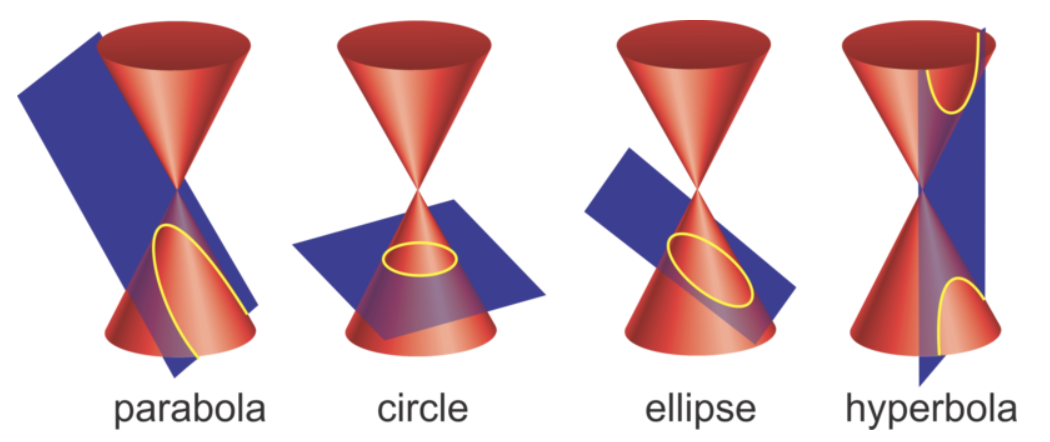
\includegraphics[width=0.65\textwidth]{images/conics.png}
	\end{figure}

\begin{itemize}
\item The set of real solutions to these polynomials are circles, ellipses, parabolas, hyperbolas, and degenerate cases like a point or pair of lines. Therefore, we seek `nice' points on these surfaces.

\item We want our curves to be smooth, i.e. there is no solution (over $\C^2$) to
	\[
	F(x,y)= \dfrac{\partial F}{\partial x}(x,y)= \dfrac{\partial F}{\partial y}(x,y)= 0
	\]
\end{itemize}

\end{frame}



% Examples
\begin{frame}[plain,t]
\frametitle{\textcolor{white}{Finding Rational Points on Conics}}
	\[
	x^2 + y^2 = 1 
	\] \vfill
	\[
	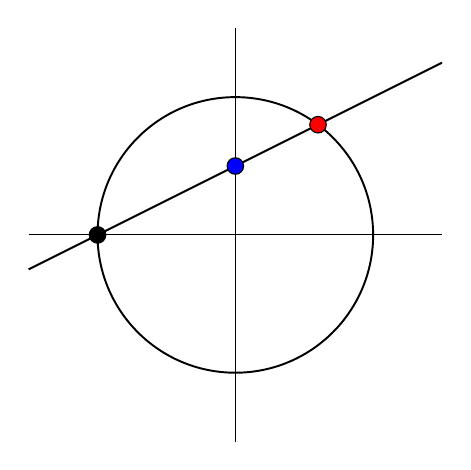
\begin{tikzpicture}[scale=1.75]
	\draw (-1.5,0) -- (1.5,0);
	\draw (0,-1.5) -- (0,1.5);

	\draw[line width=0.7] (-1.5,-0.25) -- (1.5,1.25);
	\draw[line width=0.7] (0,0) circle (1);
	
	\draw[fill=black] (-1,0) circle (0.06);
	\draw[fill=blue] (0,0.5) circle (0.06);
	\draw[fill=red] (0.6,0.8) circle (0.06);
	\end{tikzpicture}
	\] \vfill
	\[
	C(\Q)= \{ (-1,0) \} \cup \left\{ \left(\dfrac{1-t^2}{1+t^2}, \dfrac{2t}{1+t^2} \right) \colon t \in \Q \right\}
	\] \pspace
\end{frame}



% Local-to-Global
\begin{frame}[plain] \frametitle{Local-Global Principles}
The `projection' method does not always work---we need a rational point at the start. For example, the following circle has no rational point:
	\[
	x^2 + y^2= 3
	\]
Transforming this into an integer equation, one can work modulo 4 and show there is no solution, which implies there is no rational solution. In fact, all conics that do not have a rational point fail some type of congruence condition. 

\begin{prin}[Hasse, Local-Global Principle]
A collection of equations has a solution `if and only if' it has a solution in $\R$ and $\Q_p$ for all $p$.
\end{prin} 
\end{frame}



% Falting's Theorem
\begin{frame}[plain] \frametitle{The Case of Higher Degree Equations} \small

\begin{thm}[Mordell, 1922, Faltings, 1983]
If $\mathcal{C}$ is a curve over $\Q$ of genus $g$ at least 2, then $\mathcal{C}$ has at most finitely many rational points. 
\end{thm}

	\begin{figure}[ht]
	\centering
	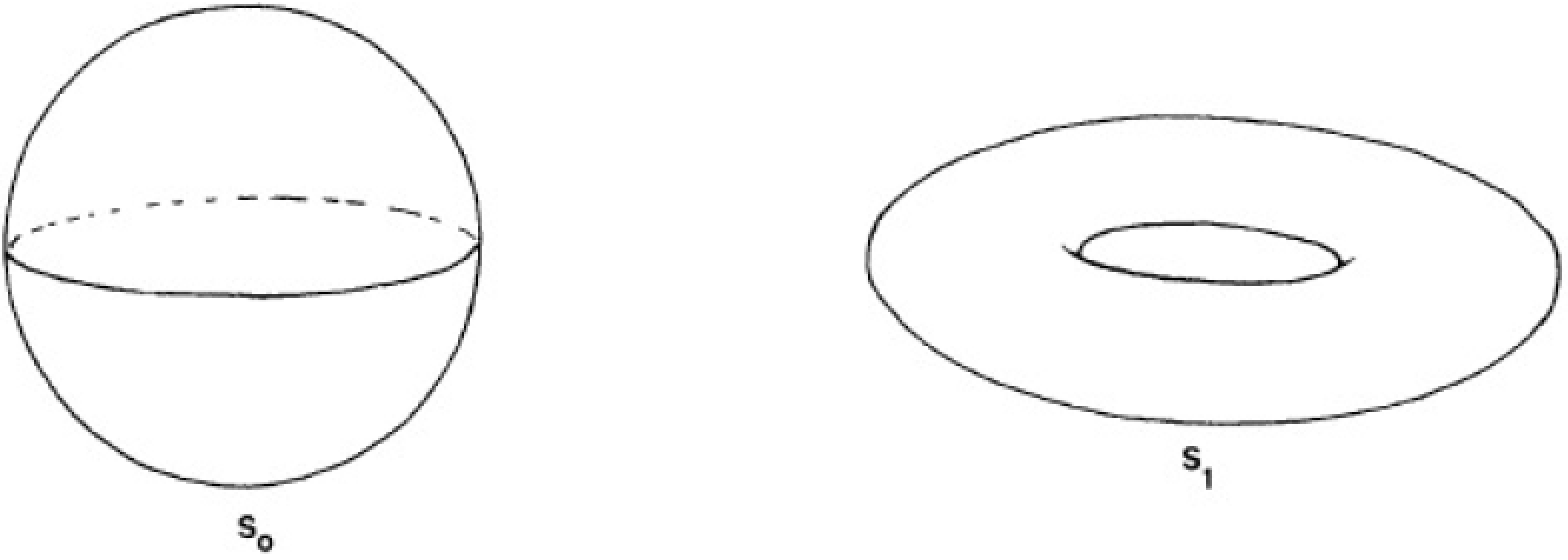
\includegraphics[width=0.35\textwidth]{images/genus1.png} \quad
	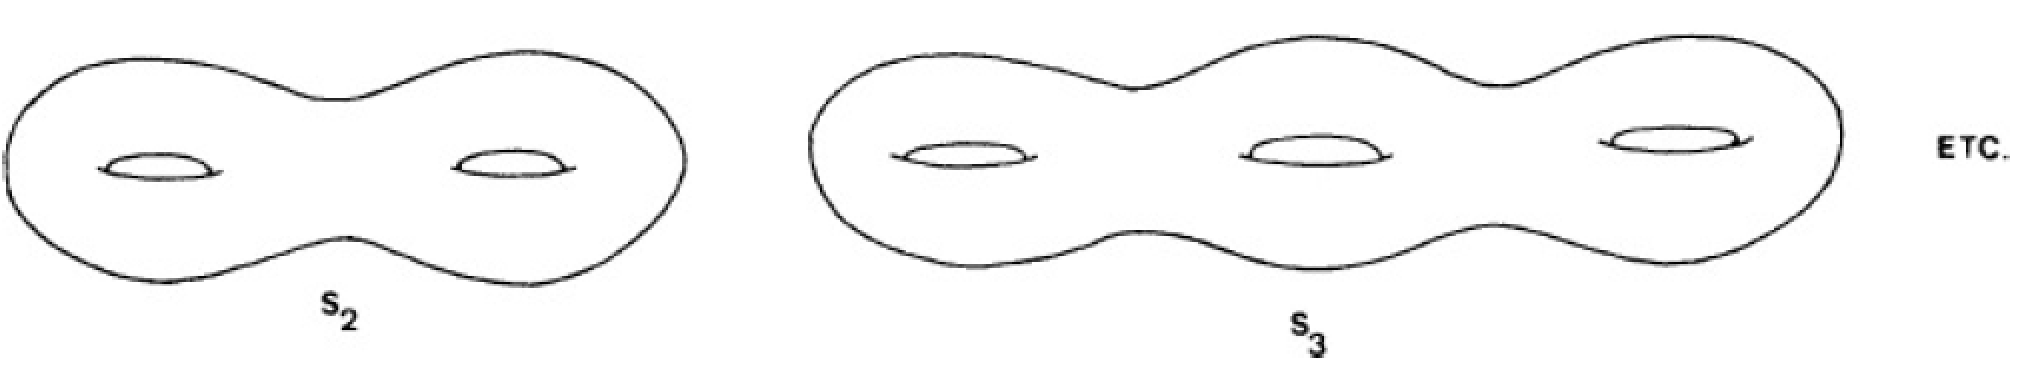
\includegraphics[width=0.45\textwidth]{images/genus2.png}
	\end{figure}

\begin{rem}
If $\mathcal{C}$ is a nonsingular, projective plane curve of degree $d$ is given by\dots
	\[
	g= \dfrac{(d - 1)(d - 2)}{2}
	\]
For a non-singular hypersurface $H$ of degree $d$ in $\mathbb{P}^n$, we have $g= \binom{d - 1}{n}$. Topologically, the genus is the number of `holes.' 
\end{rem}
\end{frame}



% Isosceles Triangle Problem
\begin{frame} \frametitle{Isosceles Triangle Problem} \footnotesize
{\itshape Does there exist a rational right triangle and a rational isosceles triangle that have the same area and the same perimeter?} \pspace

If yes, we can find $t, u \in \Q$, $0 < t < 1$, $0 < u < 1$, and $k > 0$. 
	
	\begin{figure}[!ht]
	\centering
	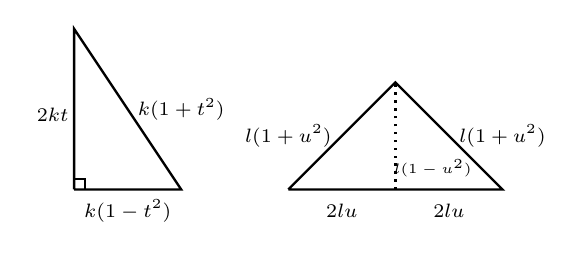
\begin{tikzpicture}[scale=0.68]
	\draw[line width=0.03cm] (0,0) -- (0,3) -- (2,0) -- (0,0);
	\draw[line width=0.03cm] (0,0.2) -- (0.2,0.2) -- (0.2,0);
	\node at (1,-0.4) {\scriptsize$k(1-t^2)$};
	\node at (-0.4,1.4) {\scriptsize$2kt$};
	\node at (2.0,1.5) {\scriptsize$k(1+t^2)$};
	
	\draw[line width=0.03cm] (4,0) -- (6,2) -- (8,0) -- (4,0);
	\draw[line width=0.03cm,dotted] (6,0) -- (6,2);
	%\draw[line width=0.03cm] (5.85858,1.85858) -- (6,1.71716) -- (6.14142,1.85858);
	\node at (4,1) {\scriptsize$l(1+u^2)$};
	\node at (8,1) {\scriptsize$l(1+u^2)$};
	\node at (5,-0.4) {\scriptsize$2lu$};
	\node at (7,-0.4) {\scriptsize$2lu$};
	\node at (6.7,0.4) {\tiny$l(1-u^2)$};
	\end{tikzpicture}
	\end{figure} 
With even more algebra, this is the same as finding a rational solution $(x,y)$ to 
	\[
	y^2= x^6 + 12x^5 - 32x^4 + 52x^2 - 48x + 16
	\]

\begin{thm}[Hirakawa, Matsumura 2018]
Up to similitude, there exists a unique pair of rational right triangles and a rational isosceles triangle which have the same perimeter and the same area. The unique pair consists of the right triangle with side $(377,135,352)$. and isosceles triangle with sides $(366,366,132)$. 
\end{thm}
\end{frame}



% Sweet Spot
\begin{frame}[plain]
\ctext{This leaves the `sweet spot' of cubic equations}
\end{frame}



% Elliptic Curves
\begin{frame}[plain]
\ctext{Elliptic Curves}
\end{frame}



% Quote
{\setbeamertemplate{background canvas}{
\tikz[remember picture,overlay]
	\node[opacity=0.3] at (current page.center) {
	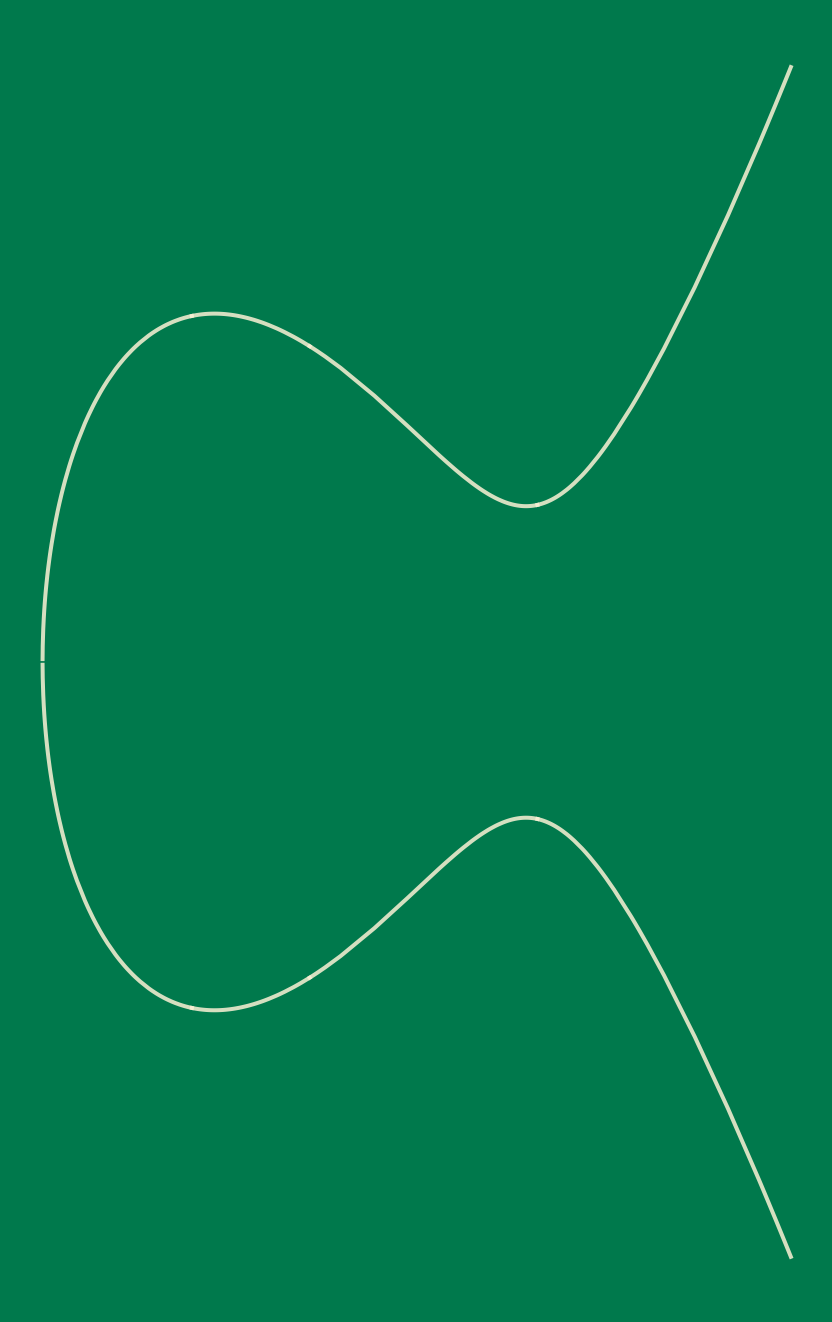
\includegraphics[width=1.25\paperwidth,
	height=1.25\paperheight]{images/curve2.png}};} 
\begin{frame}[plain]
	\begin{minipage}{0.18\textwidth}
 	\begin{figure}[h]
	\centering
	\fbox{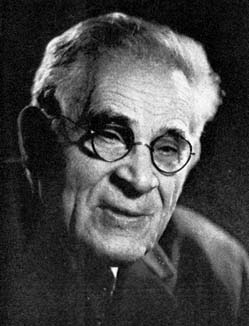
\includegraphics[width=1.1\textwidth]{images/mordell.jpg}} \par
	{\small 1888 -- 1972}
	\end{figure}
	\end{minipage} \hspace{0.2cm} \begin{minipage}{0.76\textwidth}
	\begin{center} \phantom{.} \par \phantom{.} \par
	{\itshape ``Mathematicians have been familiar with very few questions for so long a period with so little accomplished in the way of general results, as that of finding the rational [points on elliptic curves].''} \\
	 \phantom{x}\hfill-- L.J. Mordell, 1922
	\end{center}
 	\end{minipage}
\end{frame}
}



% Elliptic Curves
% !TEX root = ../swarthmore_talk.tex

% Elliptic Curves
\begin{frame}[plain] 
\ctext{Elliptic Curves}
\end{frame}



% EC Definition
\begin{frame}[plain]
\begin{dfn}[Elliptic Curve]
An elliptic curve is\dots
\begin{itemize}
\item A nonsingular projective curve of genus 1.
\item An abelian variety of dimension 1.
\item A nonempty smooth variety, $V(F)$, with $\deg F=3$.
\item A compact Riemann surface of genus 1.
\item The set of solutions to\dots
	\[
	y^2 + a_1 xy + a_3y = x^3 + a_2 x^2 + a_4 x + a_6
	\]
along with a specified `distinguished point $\infty$' and an addition law given by the chord-tangent law.
\end{itemize}
\end{dfn}
\end{frame}



% Cubic Functions/Elliptic Curves
\begin{frame}[plain] \frametitle{Elliptic Curves --- Short Weierstrass Form}
	\[
	y^2 + a_1 xy + a_3y = x^3 + a_2 x^2 + a_4 x + a_6
	\] \pspace 

\begin{itemize}
\item Make the substitution $y \mapsto y + \dfrac{a_1 x+a_3}{2}$.
\item Obtain $y^2= x^3+ a_2' x^2 + a_4' x + a_6'$
\item Make the substitution $x \mapsto x + \dfrac{a_2'}{3}$
\end{itemize} \pspace 
	\[
	\star \enskip \boxed{E_{A,B}: y^2 = x^3 + Ax + B} \enskip \star
	\] \pspace

\begin{itemize}
\item Require $\Delta= -16(4A^3+27B^2) \neq 0$.
\item $C(\Q)$ could be empty, finite, or infinite. 
\end{itemize}
\end{frame}



% Real Plot 
\begin{frame}[plain]
	\begin{figure}[h]
	\centering
	\begin{subfigure}{0.30\textwidth}
	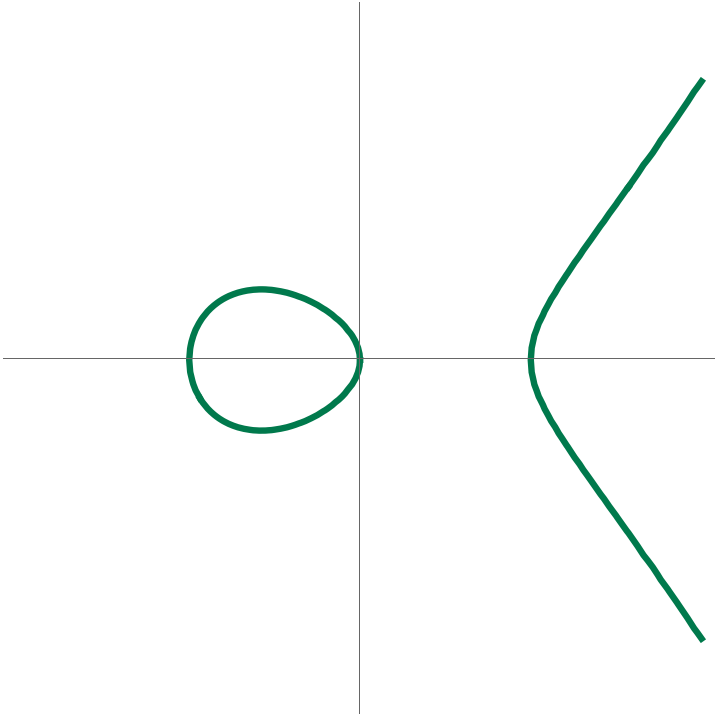
\includegraphics[width=\textwidth]{images/ec1.png}
	\caption*{$y^2 = x(x + 1)(x - 1)$}
	\end{subfigure} \qquad\qquad
	%
	\begin{subfigure}{0.30\textwidth}
	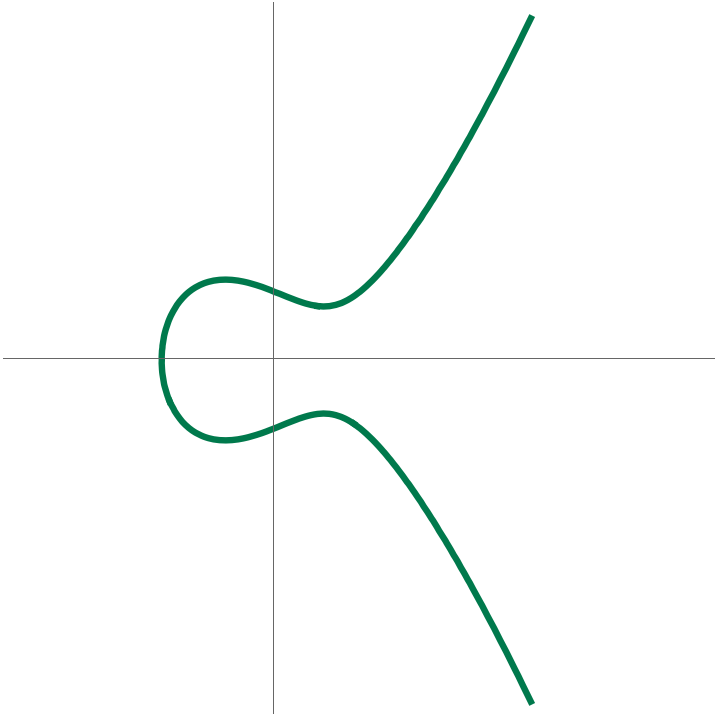
\includegraphics[width=\textwidth]{images/ec2.png}
	\caption*{$y^2 = x^3 - x + 1$}
	\end{subfigure}
	\end{figure}
	%
	\begin{figure}
	\centering
	\begin{subfigure}{0.30\textwidth}
	
\includegraphics[width=\textwidth]{images/ec3.png}
	\caption*{$y^2 = x^2 (x + 1)$}
	\end{subfigure} \qquad\qquad
	%
	\begin{subfigure}{0.30\textwidth}
	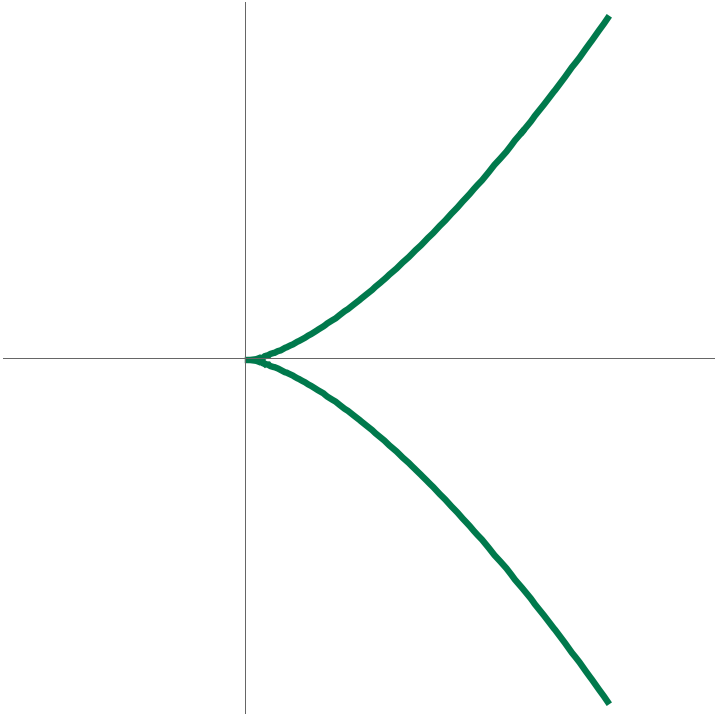
\includegraphics[width=\textwidth]{images/ec4.png}
	\caption*{$y^2= x^3$}
	\end{subfigure}
	\end{figure}
\end{frame}



% Torus
\begin{frame}[plain]
\scriptsize In fact, if one considers the complex solutions to these equations, one can show that $E(\C)$ is isomorphic to a torus!

	\begin{figure}[!ht]
	\centering
	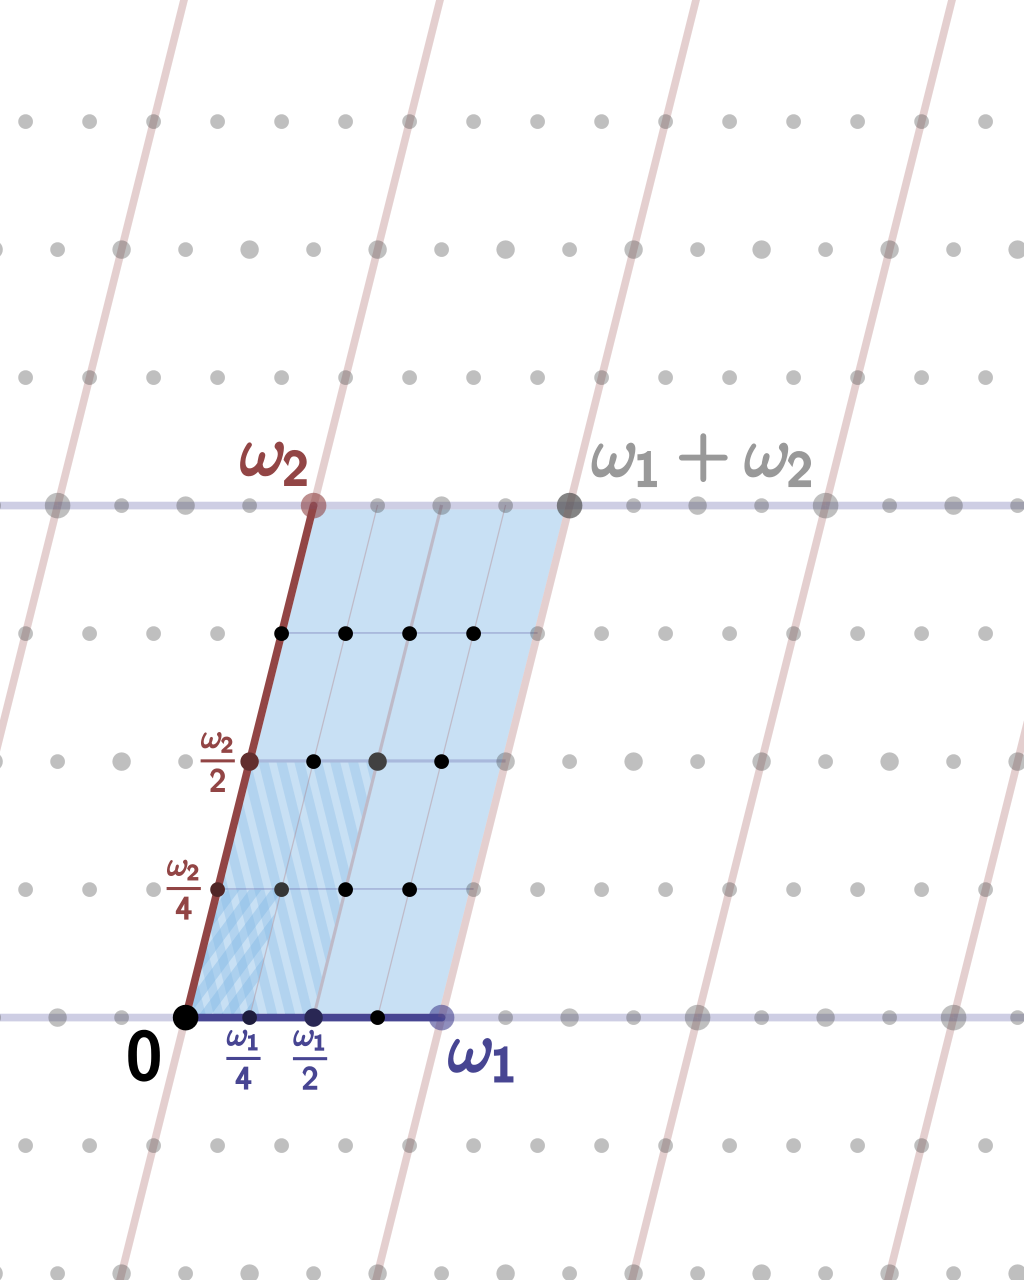
\includegraphics[width=0.25\textheight]{images/lattice.png} \qquad\qquad
	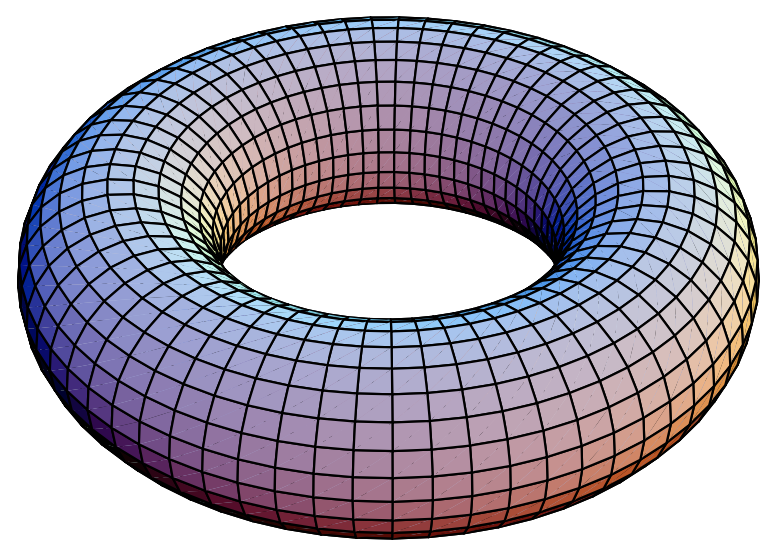
\includegraphics[width=0.25\textwidth]{images/torus.png}
	\end{figure}\fn{\tiny S. Derbyshire, \emph{Lattice torsion points}. CC BY-SA 3.0}

	\begin{figure}[!ht]
	\centering
	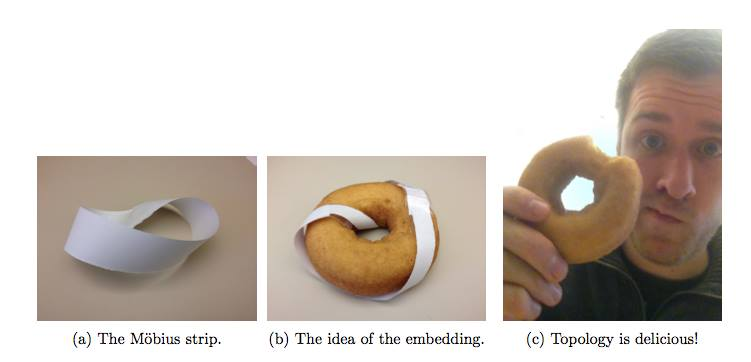
\includegraphics[width=0.8\textheight]{images/delicious.jpg}
	\end{figure}
\end{frame}



% Group & Fields
\begin{frame}[plain]
\ctext{Groups \& Fields}
\end{frame}



% Groups
\begin{frame}[plain] \frametitle{What is a Group?} \small
\begin{dfn}[Group]
A group, $G$, is a set with a binary operation, $\star$, such that\dots
	\begin{enumerate}[(a)]
	\item (Associativity) $g \star (h \star k)= (g \star h) \star k$ for all $g, h, k \in G$.
	\item (Identity) There exists $e \in G$ such that $e \star g= g \star e= g$ for all $g \in G$.
	\item (Inverses) For every $g \in G$, there exists $g^{-1} \in G$ such that $g \star g^{-1}= g^{-1} \star g= e$. 
	\end{enumerate}
\end{dfn}

\begin{ex}
\begin{enumerate}[(i)]
\item The integers under addition modulo $n$ form a group, i.e. `clock arithmetic.' 
	\[
	\begin{tikzpicture}[scale=0.7]
        \draw[thick,SwarthGarnet] (0,0) circle (1);
        \draw[thick,SwarthGarnet] (0.8,0) -- (1,0);
        \draw[thick,SwarthGarnet] (0.693,0.4) -- (0.867,0.5);
        \draw[thick,SwarthGarnet] (0.4,0.693) -- (0.5,0.866);
        \draw[thick,SwarthGarnet] (0,0.8) -- (0,1);
        \draw[thick,SwarthGarnet] (-0.4,0.692) -- (-0.5,0.866);
        \draw[thick,SwarthGarnet] (-0.693,0.4) -- (-0.866,0.5);
        \draw[thick,SwarthGarnet] (-0.8,0) -- (-1,0); 
        \draw[thick,SwarthGarnet] (-0.693,-0.4) -- (-0.866,-0.5);
        \draw[thick,SwarthGarnet] (-0.4,-0.693) -- (-0.5,-0.866);
        \draw[thick,SwarthGarnet] (0,-0.8) -- (0,-1);
        \draw[thick,SwarthGarnet] (0.4,-0.693) -- (0.5,-0.866);
        \draw[thick,SwarthGarnet] (0.692,-0.4) -- (0.866,-0.5);
        
        \draw[fill=blue] (0,0) circle (0.05);
        
        \draw[very thick,white] (0,0) -- (0.247,0.761);
        \draw[thick,blue] (0,0) -- (0.247,0.761);
        
        \draw[very thick,white] (0,0) -- (0.298,-0.183);
        \draw[thick,blue] (0,0) -- (0.298,-0.183);
        \end{tikzpicture}
        \]

\item The integers, $\mathbb{Z}$, under addition form a group, i.e. an `infinite clock.'
\end{enumerate}
\end{ex}
\end{frame}



% Torsion
\begin{frame}[plain] \frametitle{Torsion Subgroups} \small

\begin{dfn}[Torsion]
A group element which when operated on itself a finite number of times returns to the identity is called a \textit{torsion} element. The torsion subgroup of a group is the collection of all its torsion elements.
\end{dfn} \par\vspace{0.3cm}

From now on, when you hear $n$-torsion, think a clock with $n$ numbers on it, which we will denote $\mathbb{Z}/n\mathbb{Z}$. If there is a `$\oplus$' symbol between them, just imagine two of these types of clocks next to each other---ticking away.
	\[
	\begin{tikzpicture}[scale=0.7]
        \draw[thick,SwarthGarnet] (0,0) circle (1);
        \draw[thick,SwarthGarnet] (0.8,0) -- (1,0);
        \draw[thick,SwarthGarnet] (0.693,0.4) -- (0.867,0.5);
        \draw[thick,SwarthGarnet] (0.4,0.693) -- (0.5,0.866);
        \draw[thick,SwarthGarnet] (0,0.8) -- (0,1);
        \draw[thick,SwarthGarnet] (-0.4,0.692) -- (-0.5,0.866);
        \draw[thick,SwarthGarnet] (-0.693,0.4) -- (-0.866,0.5);
        \draw[thick,SwarthGarnet] (-0.8,0) -- (-1,0); 
        \draw[thick,SwarthGarnet] (-0.693,-0.4) -- (-0.866,-0.5);
        \draw[thick,SwarthGarnet] (-0.4,-0.693) -- (-0.5,-0.866);
        \draw[thick,SwarthGarnet] (0,-0.8) -- (0,-1);
        \draw[thick,SwarthGarnet] (0.4,-0.693) -- (0.5,-0.866);
        \draw[thick,SwarthGarnet] (0.692,-0.4) -- (0.866,-0.5);
        
        \draw[fill=blue] (0,0) circle (0.05);
        \draw[very thick,blue] (0,0) -- (0.4,0.693);
      
	\node at (1.65,0) {`$=$'};
	\node at (3,0) {$\mathbb{Z}/12\mathbb{Z}$};

	\tikzset{shift={(6,0)}}

        \draw[thick,SwarthGarnet] (0,0) circle (1);
        \draw[thick,SwarthGarnet] (0,0.8) -- (0,1);
        \draw[thick,SwarthGarnet] (0,-0.8) -- (0,-1);
        
        \draw[fill=blue] (0,0) circle (0.05);
        \draw[very thick,blue] (0,0) -- (0,0.8);
        
        \tikzset{shift={(2.5,0)}}
        	
        \draw[thick,SwarthGarnet] (0,0) circle (1);
        \draw[thick,SwarthGarnet] (0.8,0) -- (1,0);
        \draw[thick,SwarthGarnet] (0.693,0.4) -- (0.867,0.5);
        \draw[thick,SwarthGarnet] (0.4,0.693) -- (0.5,0.866);
        \draw[thick,SwarthGarnet] (0,0.8) -- (0,1);
        \draw[thick,SwarthGarnet] (-0.4,0.692) -- (-0.5,0.866);
        \draw[thick,SwarthGarnet] (-0.693,0.4) -- (-0.866,0.5);
        \draw[thick,SwarthGarnet] (-0.8,0) -- (-1,0); 
        \draw[thick,SwarthGarnet] (-0.693,-0.4) -- (-0.866,-0.5);
        \draw[thick,SwarthGarnet] (-0.4,-0.693) -- (-0.5,-0.866);
        \draw[thick,SwarthGarnet] (0,-0.8) -- (0,-1);
        \draw[thick,SwarthGarnet] (0.4,-0.693) -- (0.5,-0.866);
        \draw[thick,SwarthGarnet] (0.692,-0.4) -- (0.866,-0.5);
        
        \draw[fill=blue] (0,0) circle (0.05);
        
        \draw[very thick,blue] (0,0) -- (0.4,0.693);
      
	\node at (1.65,0) {`$=$'};
	\node at (3.8,0) {$\mathbb{Z}/2\mathbb{Z} \oplus \mathbb{Z}/12\mathbb{Z}$};
        \end{tikzpicture}
        \] \par\vspace{0.3cm}
We will denote an `infinite clock', i.e. a clock with the numbers $1, 2, \ldots$ on it, by $\mathbb{Z}$. If we write $\mathbb{Z}^r$, we just mean $r$ of these types of clocks next to each other---ticking away. 
\end{frame}



% Fields
\begin{frame}[plain] \frametitle{What is a (Galois) Field?} \footnotesize
\begin{dfn}[`Field']
A field is a collection of `numbers' where one can perform addition, subtraction, multiplication, and (nonzero) division and these operations are `nice.'
\end{dfn}

\begin{ex}
\begin{enumerate}[(i)]
\item The rational numbers, $\mathbb{Q}$, are a field with the usual $+, -, \times, \div$.
\item Number fields (extensions of $\mathbb{Q}$) are also fields. For example, consider $\Q(\sqrt{2})= \{ a + b \sqrt{2} \;|\; a, b \in \mathbb{Q} \}$,
	\[
	\begin{gathered}
	(5 - 3\sqrt{2}) + (-4 + 6 \sqrt{2})= 1 + 3 \sqrt{2} \\
	(6 - 7\sqrt{2}) \cdot (6 + 7\sqrt{2})= -62 + 0\sqrt{2} \\
	\dfrac{1 + 3\sqrt{2}}{1 + \sqrt{2}}= 5 - 2\sqrt{2}
	\end{gathered}
	\] 
The dimension of a number field as a $\mathbb{Q}$-vector space, i.e. number of `pieces' in these numbers, is called the \textit{degree} of the extension. 
\end{enumerate}
\end{ex}
\end{frame}



% Galois Fields
\begin{frame}[plain] \frametitle{Galois Fields} \footnotesize
\begin{dfn}[Galois Field]
A Galois field is a `number field' whose numbers satisfy extra symmetries. 
\end{dfn}

\begin{ex}
Consider the number field $\mathbb{Q}(i) = \{ a + bi \;|\; a, b \in \mathbb{Q} \}$, i.e. ``complex numbers with only rational parts.'' We can add, subtract, multiply, and divide these numbers. But they also have an extra symmetry given by conjugation, $\overline{a + bi}= a - bi$.
	\[
	\fbox{
	\begin{tikzpicture}[scale=0.72,every node/.style={scale=0.5}]
	\begin{axis}[
	grid=both,
	axis lines=middle,
	ticklabel style={fill=Topazolite!5!white},
	xmin= -10.5, xmax=10.5,
	ymin= -10.5, ymax=10.5,
	xtick={-10,-8,-6,-4,-2,0,2,4,6,8,10},
	ytick={-10,-8,-6,-4,-2,0,2,4,6,8,10},
	minor tick = {-10,-9,...,10},
	xlabel=\(x\),ylabel=\(y\),
	]
	\draw[draw=none,fill=red] (4,5) circle (0.25);
	\draw[dotted,red,thick] (0,0) -- (4,5);
	\node at (5.6,5.8) {\LARGE $4 + 5i$};

	\draw[draw=none,fill=blue] (4,-5) circle (0.25);
	\draw[dotted,blue,thick] (0,0) -- (4,-5);
	\node at (5.6,-6.2) {\LARGE $4 - 5i$};
	\end{axis}
	\end{tikzpicture}
	}
	\] 
\end{ex}
\end{frame}



% The Group Law: Addition on Elliptic Curves
\begin{frame}[plain]
\ctext{The Group Law: Addition on Elliptic Curves}
\end{frame}



% Addition Law
\begin{frame}
	\begin{figure}[h]
	\centering
	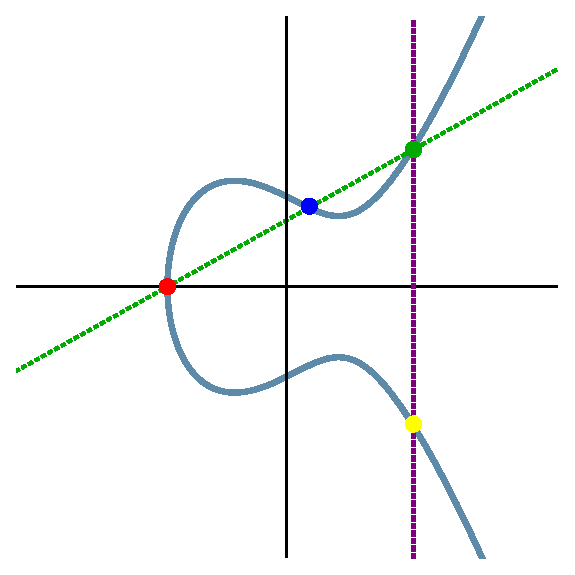
\includegraphics[width=0.75\textwidth]{images/ec_add.eps}
	\end{figure}
\end{frame}



% Why EC
\begin{frame}[plain]
\ctext{Why Elliptic Curves?}
\end{frame}



% Congruent Number Problem
\begin{frame} \frametitle{Congruent Number Problem} \scriptsize
An integer is a \textit{congruent number} if it is the area of a rational right triangle. \par\vspace{0.5\baselineskip}

\begin{minipage}{0.5\textwidth}
This is equivalent to finding a rational triplet $(x,y,z)$ with\dots
	\[
	x^2 + y^2= z^2 \quad \text{ and } \quad n= \dfrac{xy}{2}.
	\] 
\end{minipage}\begin{minipage}{0.5\textwidth}
\end{minipage}\begin{minipage}{0.5\textwidth}
	\[
	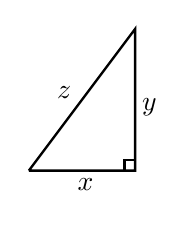
\begin{tikzpicture}[scale=0.9]
	\draw[line width=0.03cm] (0,0) -- (1.5,0) -- (1.5,2) -- (0,0);
	\draw[line width=0.03cm] (1.35,0) -- (1.35,0.15) -- (1.5,0.15);
	\node at (0.8,-0.2) {$x$};
	\node at (1.7,0.9) {$y$};
	\node at (0.5,1.1) {$z$};
	\end{tikzpicture}
	\]
\end{minipage}

\begin{ex}
\begin{itemize} \scriptsize
\item 6 is congruent: $3^2 + 4^2= 5^2$ and $\frac{3 \cdot 4}{2} = 6$
\item 5 is congruent: $\left( \frac{3}{2} \right)^2 + \left( \frac{20}{3} \right)^2= \left( \frac{41}{6} \right)^2$ and $\frac{1}{2} \left( \frac{3}{2} \cdot \frac{20}{3} \right)= 5$
\item 1 is \emph{not} congruent (due to Fermat) 
\item 157 is congruent (due to Don Zagier): \par\vspace{0.1cm}
		\scalebox{0.63}{$
	x= \dfrac{411340519227716149383203}{21666555693714761309610}, 
	y= \dfrac{6803298487826435051217540}{411340519227716149383203}, 
	z= \dfrac{224403517704336969924557513090674863160948472041}{8912332268928859588025535178967163570016480830}$
	}
\end{itemize}
\end{ex}

This problem is `equivalent' to finding rational points $(x, y)$ on the elliptic curve\dots
	\[
	y^2 = x^3 - n^2x
	\]

\end{frame}



% Fermat's Last Theorem
\begin{frame} \frametitle{Fermat's Last Theorem}
\small 

% Fermat Photos & Quotes
\begin{minipage}{0.33\textwidth}
\tiny
\begin{quote}
Cubum autem in duos cubos, aut quadratoquadratum in duos quadratoquadratos \& generaliter nullam in infinitum ultra quadratum potestatem in duos eiusdem nominis fas est dividere cuius rei demonstrationem mirabilem sane detexi. Hanc marginis exiguitas non caperet. \vspace{0.33cm}
\end{quote} 
\end{minipage}\begin{minipage}{0.33\textwidth}
	\begin{figure}
	\captionsetup{labelformat=empty}
	\centering
	\fbox{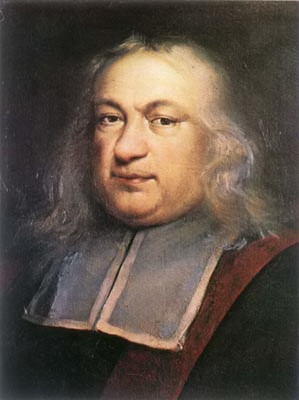
\includegraphics[width=0.55\textwidth]{images/fermat.jpeg}}
	\caption{\hspace{0.1cm}\tiny Pierre de Fermat}
	\end{figure}
\end{minipage}\begin{minipage}{0.33\textwidth} \tiny
\begin{quote}
``It is impossible to separate a cube into two cubes, or a fourth power into two fourth powers, or in general, any power higher than the second, into two powers. I have discovered a truly marvelous proof of this, which this margin is too narrow to contain.'' \vspace{0.9cm}
\end{quote}
\end{minipage}

% Theorem
\begin{thm}[{\small Fermat's Last Theorem; Wiles, 1994; Taylor-Wiles, 1995}]
There are no nontrivial integer solutions to the equation $x^n + y^n= z^n$ whenever $n > 2$.
\end{thm}

% Wiles - Taylor Photo
	\begin{figure}[h]
	\centering
	\begin{subfigure}{0.3\textwidth}
	\captionsetup{labelformat=empty}
	\centering
	\fbox{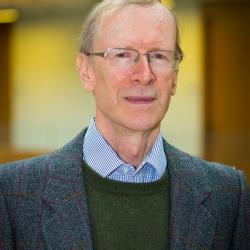
\includegraphics[width=0.64\textwidth]{images/wiles.jpg}}
	\caption{\scriptsize Andrew Wiles}
	\end{subfigure}
	%
	\begin{subfigure}{0.3\textwidth}
	\captionsetup{labelformat=empty}
	\centering
	\fbox{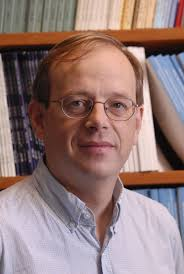
\includegraphics[width=0.43\textwidth]{images/taylor.jpeg}}
	\caption{\scriptsize Richard Taylor}
	\end{subfigure}
	\end{figure}

\end{frame}



% Sum of Three Cubes
\begin{frame}[plain,t] \frametitle{What integers are the sums of cubes?} \footnotesize
What integers $n$ are the sum of three cubes?
	\[
	x^3 + y^3 + z^3= n
	\]
\end{frame}



% Sum of Three Cubes
\begin{frame} \frametitle{What integers are the sums of cubes?} \footnotesize
	\[
	x^3 + y^3 + z^3= N
	\] \pspace

{\color{SwarthGarnet} \textbullet} From 1955 -- 2016, it was known that all integers 1--100 that were not 4 or 5 modulo 9 were the sum of three cubes except 33, 42, 74. \pspace

{\color{SwarthGarnet} \textbullet} After the release of a Numberphile video, Huisman 2016 found the following:
	{\footnotesize
	\[
	(66\,229\,832\,190\,556)^3 + (28\,3450\,105\,697\,727)^3 + (-284\,650\,292\,555\,885)^3= 74
	\]
	} \pspace
	
{\color{SwarthGarnet} \textbullet} In 2019, Booker found the following:
	{\footnotesize
	\[
	(-2\,736\,111\,468\,807\,040)^3 + (-8\,778\,405\,442\,862\,239)^3 + (8\,866\,128\,975\,287\,528)^3= 33
	\]
	} \pspace
	
{\color{SwarthGarnet} \textbullet} Finally, shortly thereafter in 2019, Sutherland and Booker (using 1.3~million hours of computing time)
	{\footnotesize
	\[
	(12\,602\,123\,297\,335\,631)^3 + (80\,435\,758\,145\,817\,515)^3 + (-80\,538\,738\,812\,075\,974)^3= 42
	\]
	}
\end{frame}



% ECDH, Playstation, Bitcoin
\begin{frame}[plain] \frametitle{ECDH, Playstation 3, \& Bitcoin} \footnotesize
Elliptic curves are the basis for ECDH (Elliptic-Curve Diffie-Hellman) encryption, which is the backbone of most modern encryption (for now\dots). 
	\begin{figure}[h]
	\centering
	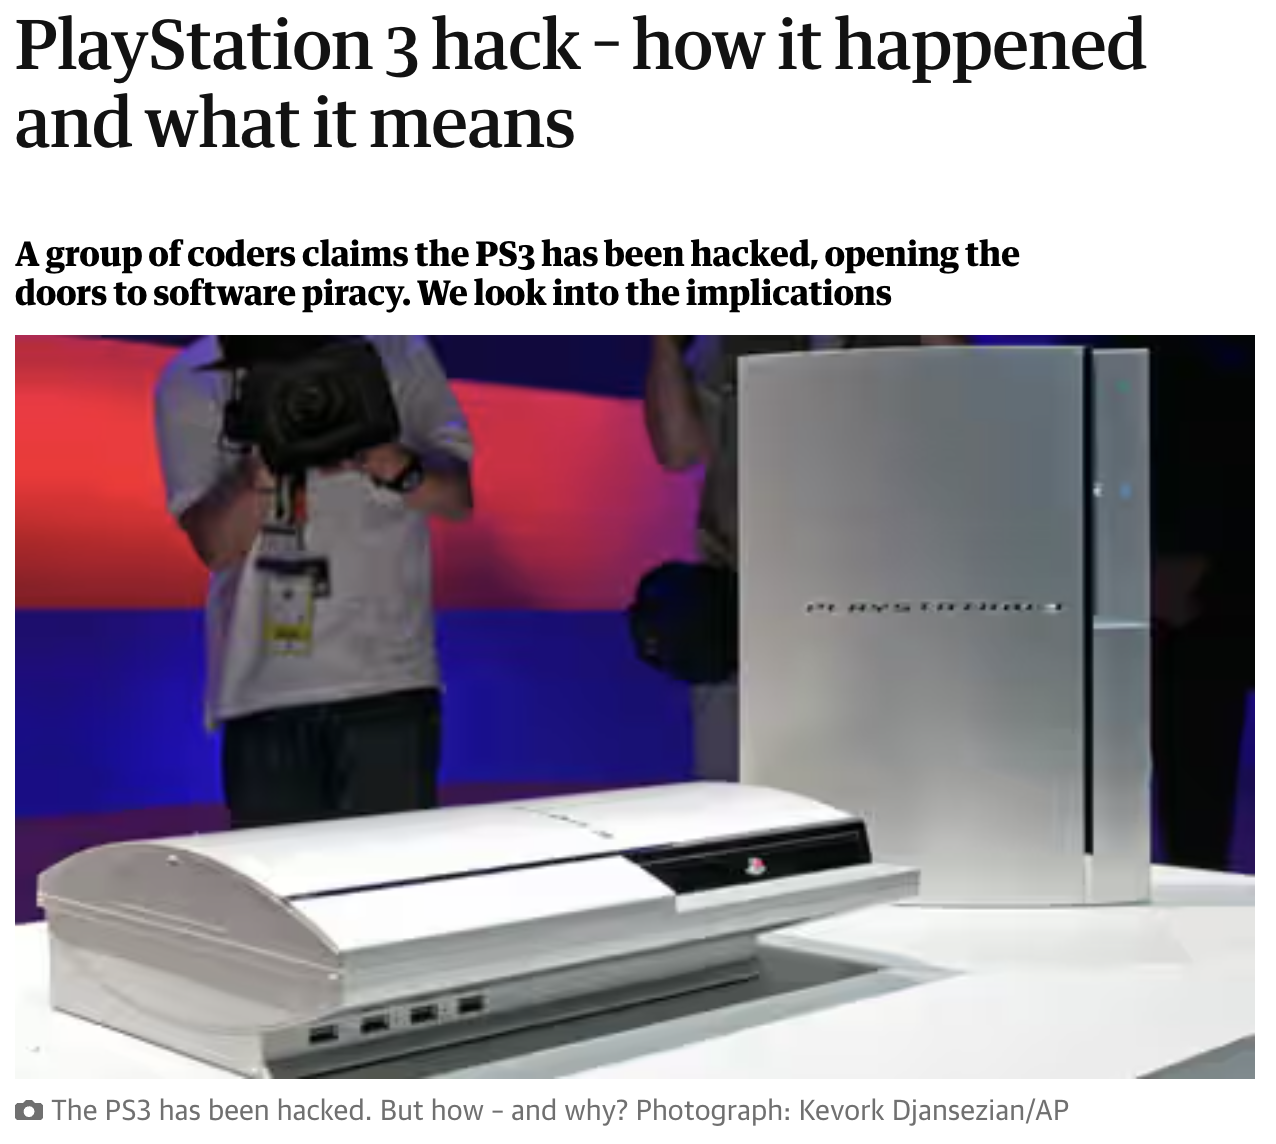
\includegraphics[width=0.515\textwidth]{images/playstation.png}
	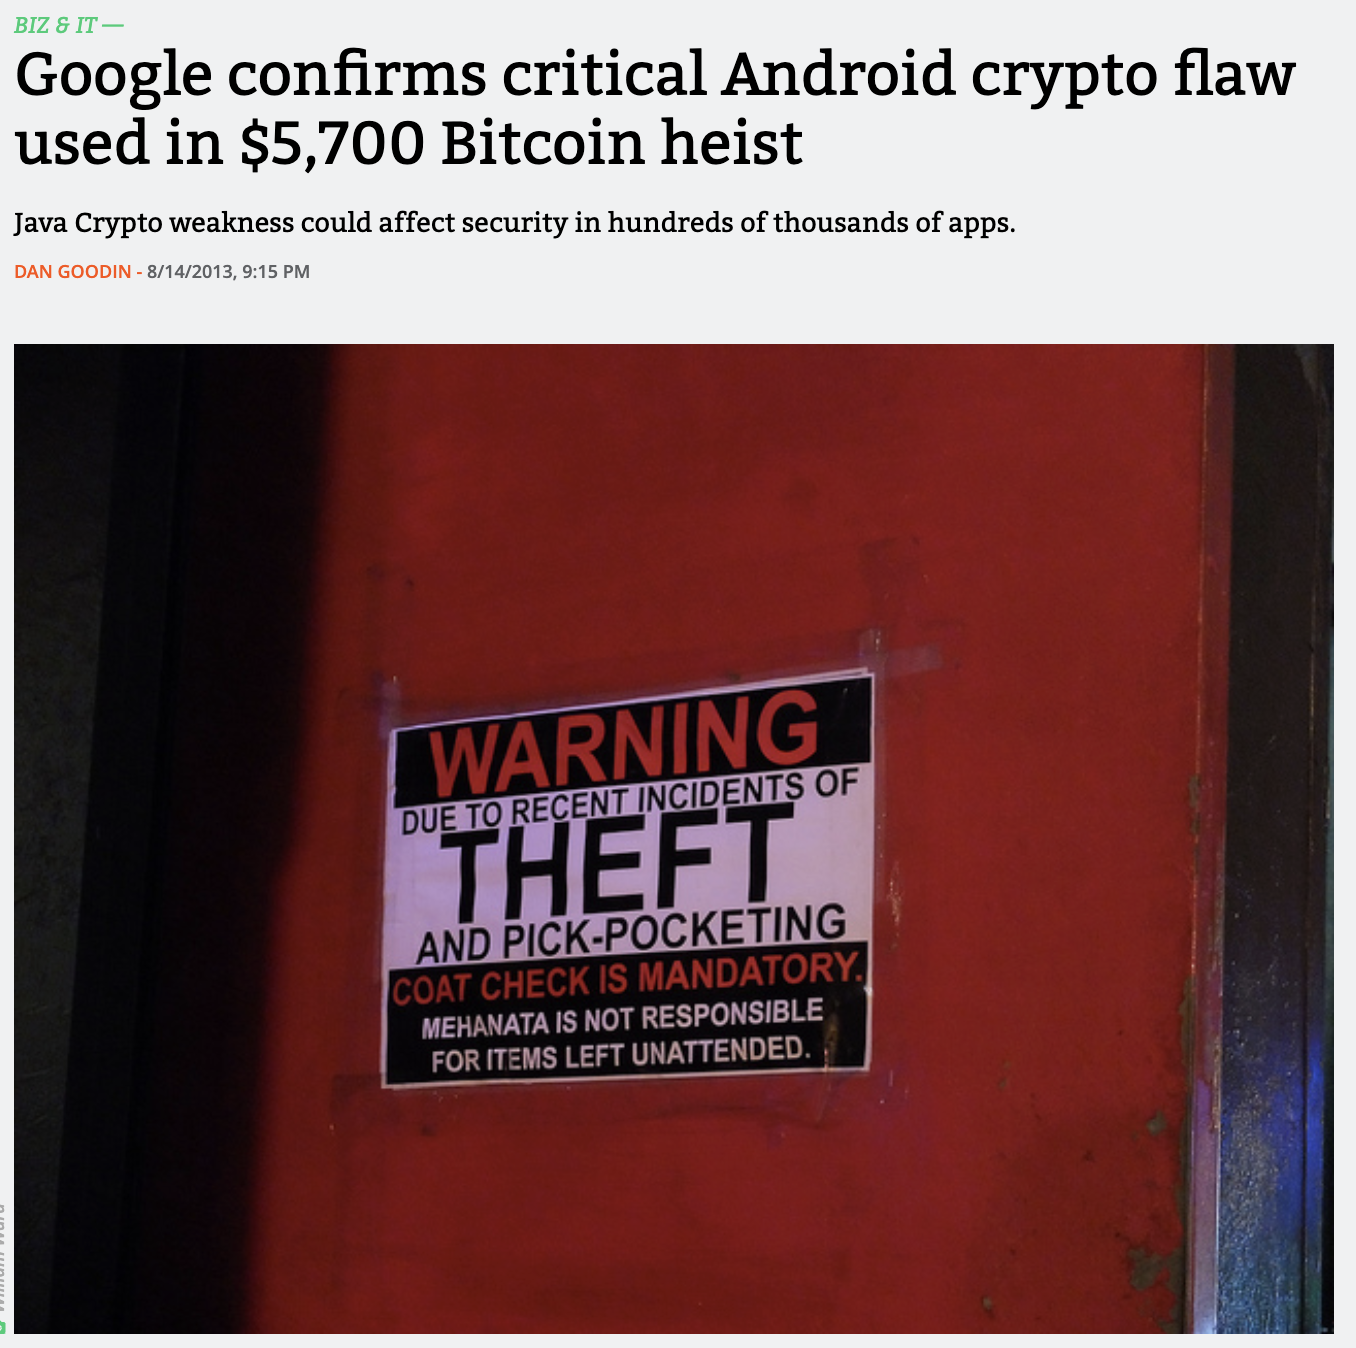
\includegraphics[width=0.475\textwidth]{images/bitcoin.png}
	\end{figure}
\end{frame}



% String Theory
\begin{frame}[plain] \frametitle{String Theory} \footnotesize
In String Theory, the idea of point-like particles are replaced by curve-like strings of some higher dimension, e.g. 6-dimensional or 23-dimensional. A single string which `moves about' and eventually returns to its start traces out a surface---specifically a torus! So paths of single strings `look like' elliptic curves! 
	\begin{figure}[ht]
	\centering
	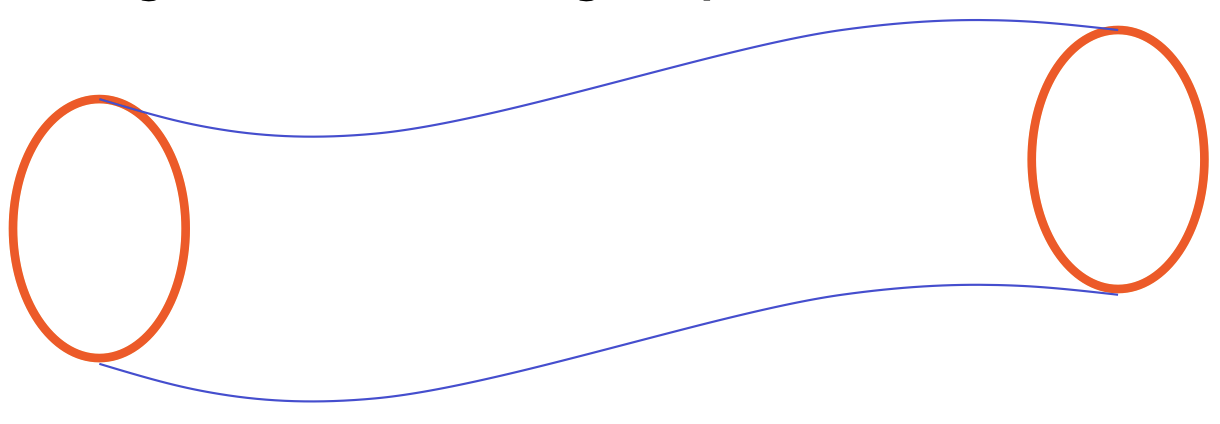
\includegraphics[width=0.35\textwidth]{images/stringpath.png}
	\end{figure}
Furthermore, in Quantum Physics, physicists often need to compute averages over all possible paths. So when considering this type of computation in String Theory, one would then be integrating over the space of all elliptic curves!
	\begin{figure}[ht]
	\centering
	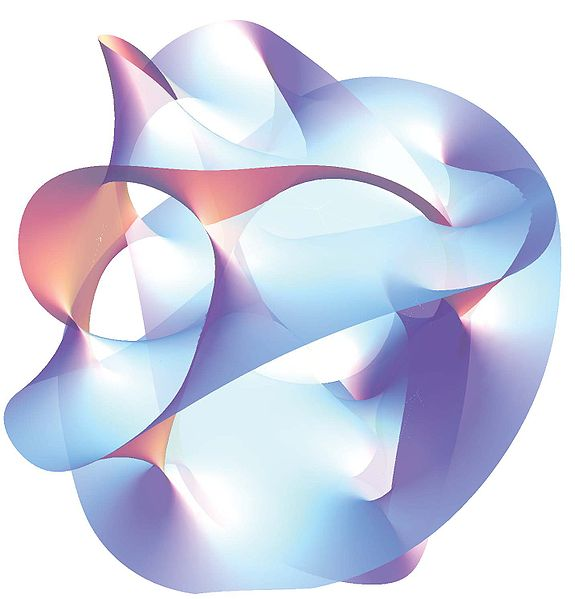
\includegraphics[width=0.30\textwidth]{images/calabi-yau.jpeg}
	\end{figure}
\end{frame}



% Moonshine
\begin{frame}[plain] \frametitle{Monstrous Moonshine} \scriptsize
An elliptic curve can be uniquely identified (over $\mathbb{C}$) by its $j$-invariant. The $j$-invariant is given by the modular $j$-invariant function,
	\[
	j(\tau)= \dfrac{1}{q} + 744 + 196884q + 214937609q^2 + \cdots
	\]
where $q= e^{2\pi i \tau}$ and $\tau$ is given by the elliptic curve. \pspace

	\begin{figure}[h]
	\centering
	\begin{subfigure}{0.20\textwidth}
	\captionsetup{labelformat=empty}
	\centering
	\fbox{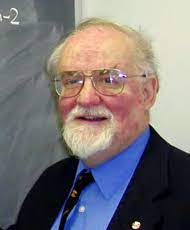
\includegraphics[width=0.62\textwidth]{images/mckay.jpeg}}
	\caption{\tiny John McKay}
	\end{subfigure} \quad
	%
	\begin{subfigure}{0.20\textwidth}
	\captionsetup{labelformat=empty}
	\centering
	\fbox{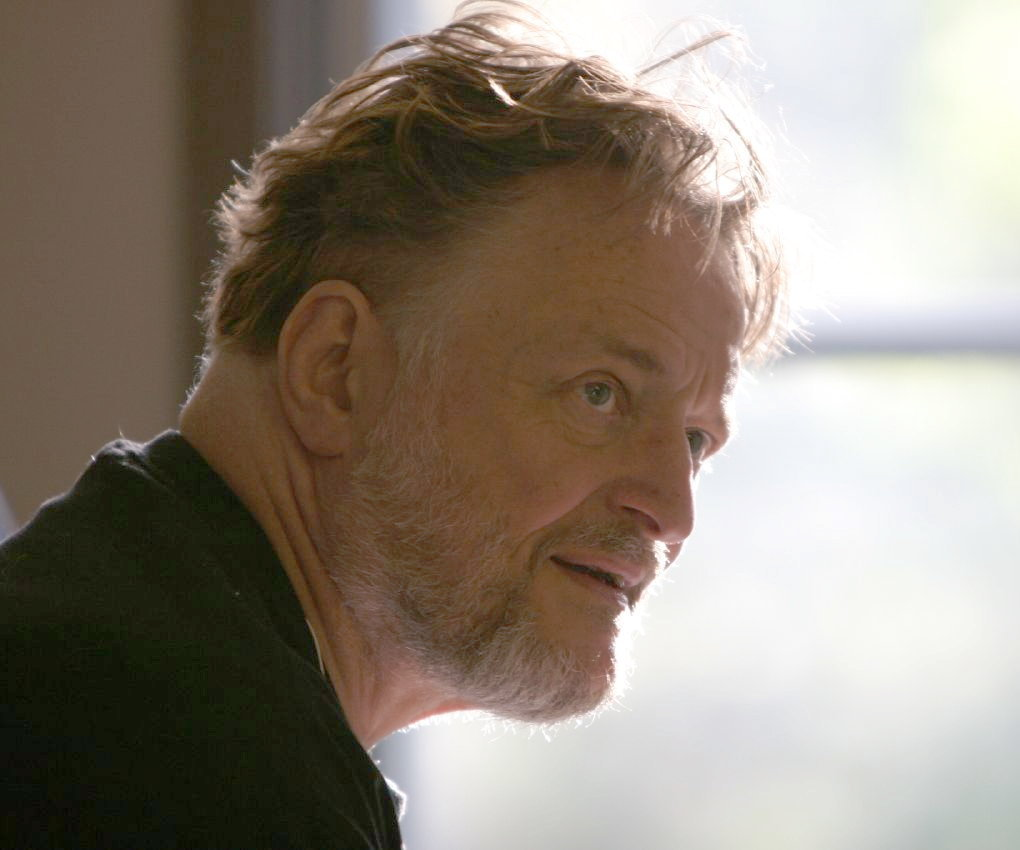
\includegraphics[width=0.9\textwidth]{images/conway.jpeg}}
	\caption{\tiny \hspace{0.2cm}John Conway}
	\end{subfigure}
	%
	\begin{subfigure}{0.20\textwidth}
	\captionsetup{labelformat=empty}
	\centering
	\fbox{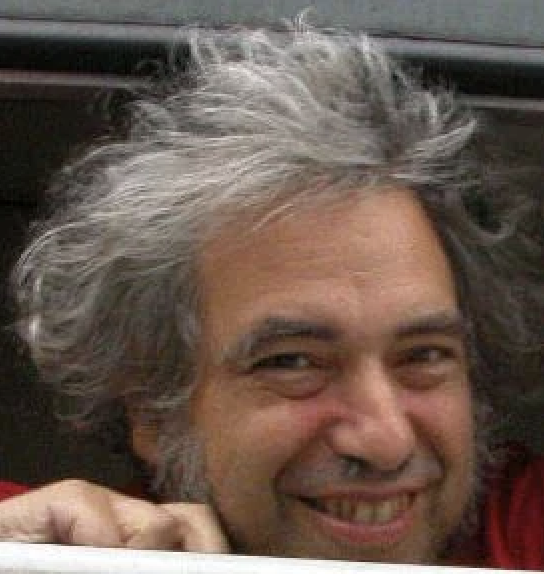
\includegraphics[width=0.71\textwidth]{images/norton.png}}
	\caption{\tiny \hspace{0.2cm}Simon Norton}
	\end{subfigure} \quad
	%
	\begin{subfigure}{0.20\textwidth}
	\captionsetup{labelformat=empty}
	\centering
	\fbox{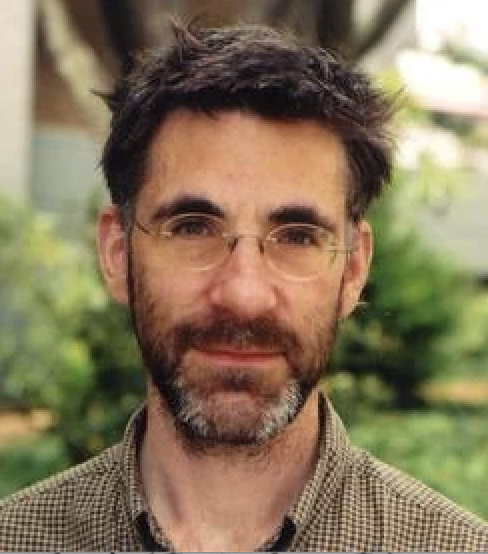
\includegraphics[width=0.665\textwidth]{images/borcherds.png}}
	\caption{\tiny Richard Borcherd}
	\end{subfigure}
	\end{figure}

Beginning In 1978, John McKay, Conway-Norton, and Borcherds discovered that the coefficients in the modular $j$-invariant are sums of linear combinations of the dimensions of the irreducible representations of the monster group, $M$, which is the largest of the sporadic groups. These appear in the classification of all finite simple groups. In fact, Borcherd's work won a Field's Medal. \pspace

This is also related to the fact that\dots
	\[
	e^{\pi \sqrt{163}} \approx 262537412640768743.99999999999925007\dots
	\]
\end{frame}



% Art
\begin{frame}[plain] \frametitle{Art} \footnotesize
Lenstra \& de Smit were recently able to finish an incomplete piece of M.C. Escher using elliptic curves:
	\begin{figure}[ht]
	\centering
	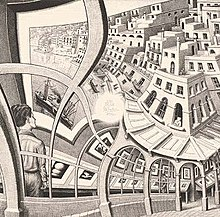
\includegraphics[width=0.482\textwidth]{images/escher2.jpg}
	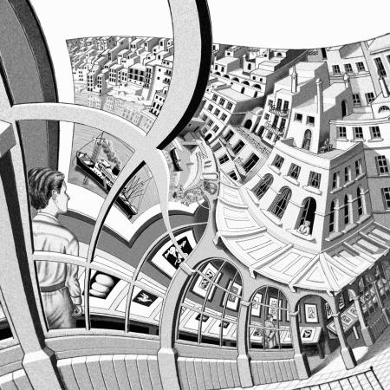
\includegraphics[width=0.478\textwidth]{images/escher_lenstra.jpeg}
	\end{figure}
\end{frame}



% Lang Quote
{\setbeamertemplate{background canvas}{
\tikz[remember picture,overlay]
	\node[opacity=0.3] at (current page.center) {
	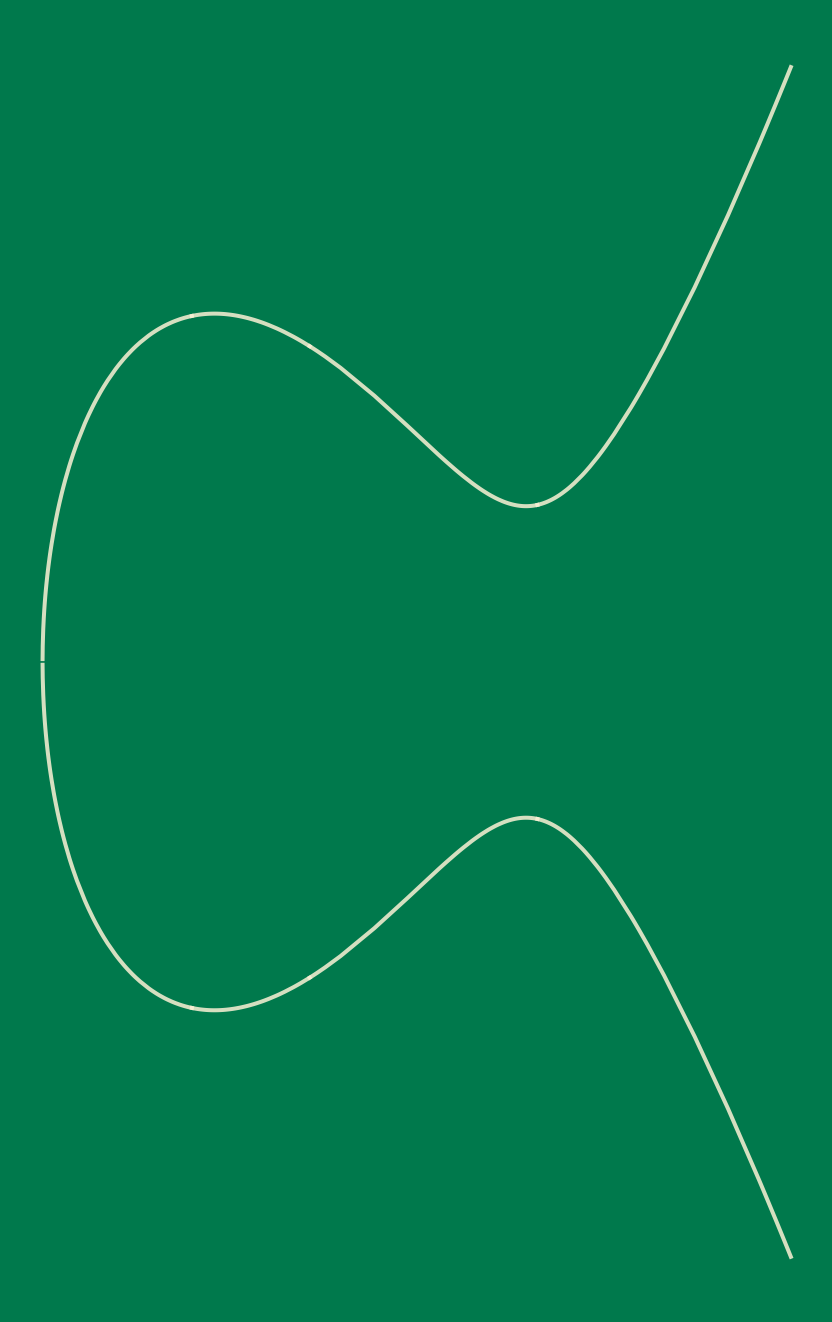
\includegraphics[width=1.25\paperwidth,
	height=1.25\paperheight]{images/curve2.png}};} 
\begin{frame}[plain]
	\begin{minipage}{0.18\textwidth}
 	\begin{figure}[h]
	\centering
	\fbox{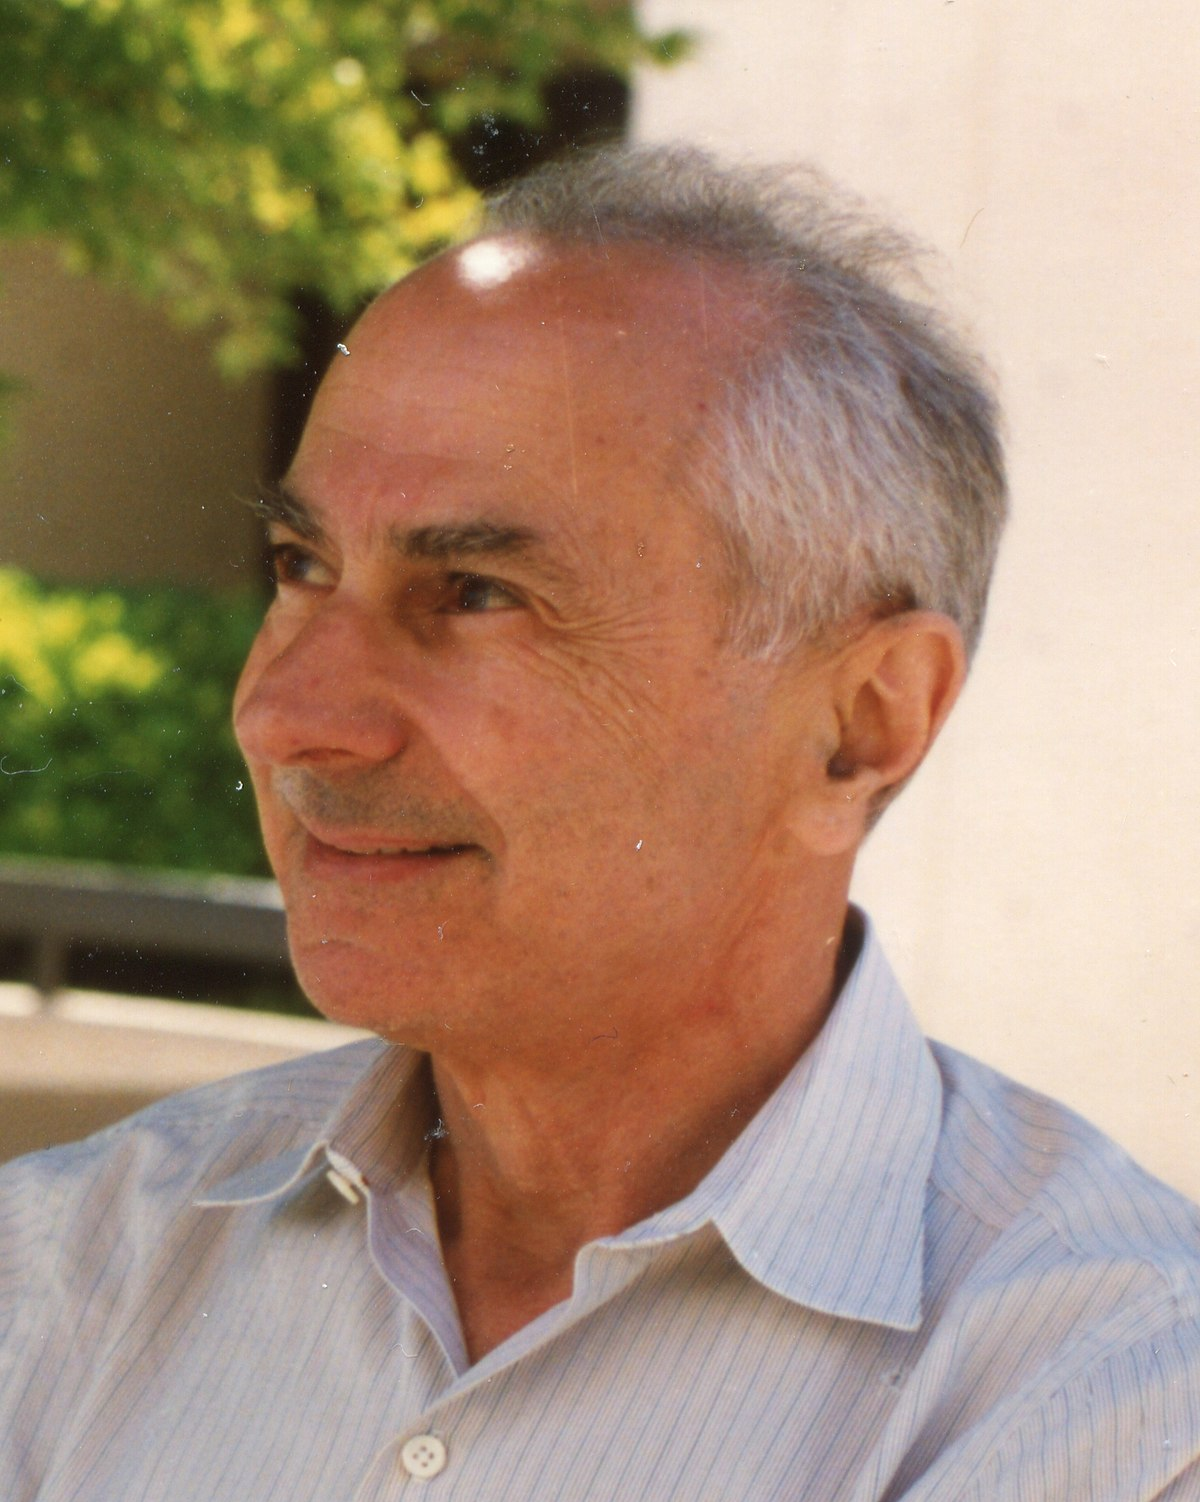
\includegraphics[width=1.1\textwidth]{images/lang.jpeg}} \par
	{\small 1927 -- 2005}
	\end{figure}
	\end{minipage} \hspace{0.2cm} \begin{minipage}{0.76\textwidth}
	\begin{center} \phantom{.} \par \phantom{.} \par
	{\itshape ``It is possible to write endlessly on elliptic curves. (This is not a threat.)''} \\
	 \phantom{x}\hfill-- Serge Lang, \textit{Elliptic Curves: Diophantine Analysis}
	\end{center}
 	\end{minipage}
\end{frame}
}



% What about Structure?
\begin{frame}[plain]
\ctext{Elliptic Curve Structure}
\end{frame}



% Mordell - Weil - Neron
\begin{frame}
	\begin{thm}[Mordell-Weil-N\'eron, 1952]
	Let $K$ be a field that is finitely generated over its prime field, and let $A/K$ be an abelian variety. Then the group of $K$-rational points on $A$, denoted $A(K)$, is a finitely generated abelian group. In particular,
		\[
		A(K) \cong \Z^{r_K} \oplus A(K)_\tors,
		\]
	where $r_K \geq 0$ is the rank and $A(K)_\tors$ is the torsion subgroup. 
	\end{thm}
	\begin{figure}[h]
	\centering
	\begin{subfigure}{0.3\textwidth}
	\captionsetup{labelformat=empty}
	\centering
	\fbox{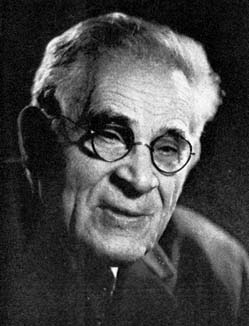
\includegraphics[width=0.8\textwidth]{images/mordell.jpg}}
	\caption{Louis J. Mordell}
	\end{subfigure}
	%
	\begin{subfigure}{0.3\textwidth}
	\captionsetup{labelformat=empty}
	\centering
	\fbox{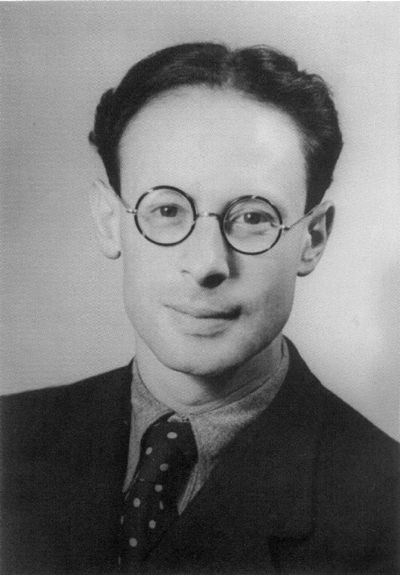
\includegraphics[width=0.74\textwidth]{images/weil.jpg}}
	\caption{Andr\'e Weil}
	\end{subfigure}
	%
	\begin{subfigure}{0.3\textwidth}
	\captionsetup{labelformat=empty}
	\centering
	\fbox{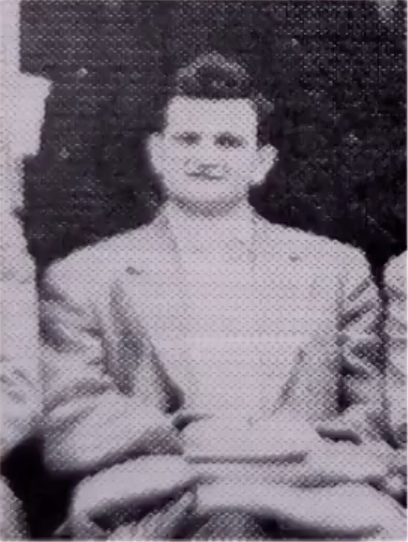
\includegraphics[width=0.8\textwidth]{images/neron.png}}
	\caption{Andr\'e N\'eron}
	\end{subfigure}
	\end{figure}
\end{frame}



% Ranks
\begin{frame}[plain] \frametitle{Ranks of Elliptic Curves (over $\Q$)}

\hspace{-0.4cm}\begin{minipage}{0.45\textwidth}
	\begin{table}[h]
	\centering
	\resizebox{!}{0.60\textwidth}{%
	\begin{tabular}{lll}  
	{\itshape\large\bfseries Rank} & {\itshape\large\bfseries Year} & {\itshape\large\bfseries Due To} \\ \hline
	3 & 1938 & Billing \\ \rowcolor{SwarthGarnet}
	\textcolor{Topazolite}{4} & \textcolor{Topazolite}{1945} &  \textcolor{Topazolite}{Wiman} \\ 
	6 & 1974 & Penney/Pomerance \\ \rowcolor{SwarthGarnet}
	\textcolor{Topazolite}{7} & \textcolor{Topazolite}{1975} & \textcolor{Topazolite}{Penney/Pomerance} \\
	8 & 1977 & Grunewald/Zimmert \\ \rowcolor{SwarthGarnet}
	\textcolor{Topazolite}{9} & \textcolor{Topazolite}{1977} & \textcolor{Topazolite}{Brumer/Kramer} \\
	12 & 1982 & Mestre \\ \rowcolor{SwarthGarnet}
	\textcolor{Topazolite}{14} & \textcolor{Topazolite}{1986} & \textcolor{Topazolite}{Mestre} \\
	15 & 1992 &  Mestre \\  \rowcolor{SwarthGarnet}
	\textcolor{Topazolite}{17} & \textcolor{Topazolite}{1992} & \textcolor{Topazolite}{Nagao} \\
	19 & 1992 & Fermigier \\ \rowcolor{SwarthGarnet}
	\textcolor{Topazolite}{20} & \textcolor{Topazolite}{1993} & \textcolor{Topazolite}{Nagao} \\
	21 & 1994 & Nagao/Kouya \\ \rowcolor{SwarthGarnet}
	\textcolor{Topazolite}{22} & \textcolor{Topazolite}{1997} & \textcolor{Topazolite}{Fermigier} \\
	23 & 1998 & Martin/McMillen \\ \rowcolor{SwarthGarnet}
	\textcolor{Topazolite}{24} & \textcolor{Topazolite}{2000} & \textcolor{Topazolite}{Martin/McMillen} \\
	28 & 2006 & Elkies \\ \rowcolor{SwarthGarnet}
	\textcolor{Topazolite}{29} & \textcolor{Topazolite}{2024} & \textcolor{Topazolite}{Elkies, Klagsbrun} \\
	\end{tabular}
	}
	\end{table}
\end{minipage} \qquad \begin{minipage}{0.35\textwidth}
	\begin{figure}
	\centering
	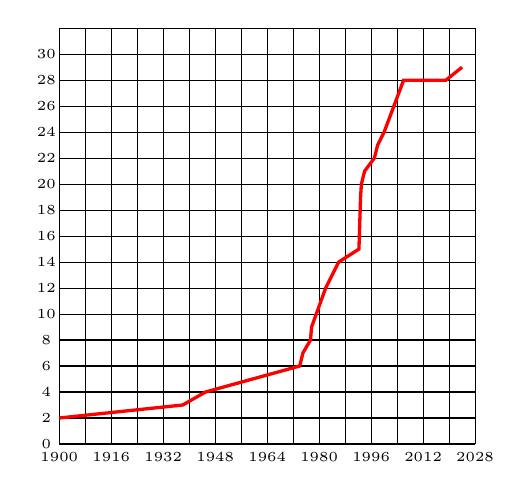
\begin{tikzpicture}[scale=0.33]%[scale=0.50, every node/.style={scale=0.1}]
	\foreach \k in {0,...,16}
		{
		\draw (\k,0) -- (\k,16);
		}
	\foreach \k in {0,...,16}
		{
		\draw (0,\k) -- (16,\k);
		}
	\node at (0,-0.5) {\tiny 1900};
	\node at (2,-0.5) {\tiny 1916};
	\node at (4,-0.5) {\tiny 1932};
	\node at (6,-0.5) {\tiny 1948};
	\node at (8,-0.5) {\tiny 1964};
	\node at (10,-0.5) {\tiny 1980};
	\node at (12,-0.5) {\tiny 1996};
	\node at (14,-0.5) {\tiny 2012};
	\node at (16,-0.5) {\tiny 2028};
	
	\node at (-0.5,0) {\tiny 0};
	\node at (-0.5,1) {\tiny 2};
	\node at (-0.5,2) {\tiny 4};
	\node at (-0.5,3) {\tiny 6};
	\node at (-0.5,4) {\tiny 8};
	\node at (-0.5,5) {\tiny 10};
	\node at (-0.5,6) {\tiny 12};
	\node at (-0.5,7) {\tiny 14};
	\node at (-0.5,8) {\tiny 16};
	\node at (-0.5,9) {\tiny 18};
	\node at (-0.5,10) {\tiny 20};
	\node at (-0.5,11) {\tiny 22};
	\node at (-0.5,12) {\tiny 24};
	\node at (-0.5,13) {\tiny 26};
	\node at (-0.5,14) {\tiny 28};
	\node at (-0.5,15) {\tiny 30};
	
	\draw[very thick,red] plot[samples=500] coordinates {
	(0,1)
	(4.75,1.5)
	(5.625,2)
	(9.25,3)
	(9.375,3.5)
	(9.6667,4)
	(9.7083,4.5)
	(10.25,6)
	(10.75,7)
	(11.5313,7.5)
	(11.5625,8.5)
	(11.5938,9.5)
	(11.625,10)
	(11.75,10.5)
	(12.125,11)
	(12.25,11.5)
	(12.5,12)
	(13.25,14)
	(14.875,14)
	(15.5,14.5)
	};
	\end{tikzpicture}
	\end{figure}
\end{minipage}
\end{frame}



% Torsion Subgroup
\begin{frame}[plain,fragile]
\ctext{Torsion Subgroups of Elliptic Curves} \small
\begin{tikzcd}[scale=0.5]
	& \left\{\begin{matrix} \text{Torsion Subgroups} \\ \text{of Elliptic Curves} \end{matrix} \right\} \arrow[<->]{dl} \arrow[<->]{dr} & \\
	\left\{\begin{matrix} \text{Galois} \\ \text{Representations} \end{matrix} \right\} \arrow[<->]{rr} & & \left\{\begin{matrix} \text{Modular} \\ \text{Curves} \end{matrix} \right\}
	\end{tikzcd}
\vfill
\end{frame}



% Q-Torsion (Mazur)
\begin{frame}[plain]
\begin{thm}[Levi-Ogg Conjecture; Mazur, 1977]
If $E/\Q$ is a rational elliptic curve, then the possible torsion subgroups $E(\Q)_\tors$ are precisely:
	\[
	\begin{cases}
	\Z/n\Z, & \text{with } n=1,2,\ldots,10,12 \text{ or} \\
	\Z/2\Z \oplus \Z/2n\Z, & \text{with } n=1,\ldots,4
	\end{cases}
	\]
Furthermore, each possibility occurs infinitely often.
\end{thm}
	\begin{figure}[h]
	\centering
	\begin{subfigure}{0.3\textwidth}
	\captionsetup{labelformat=empty}
	\centering
	\fbox{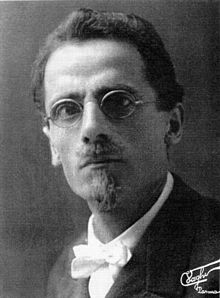
\includegraphics[width=0.72\textwidth]{images/levi.jpg}}
	\caption{Beppo Levi}
	\end{subfigure}
	%
	\begin{subfigure}{0.3\textwidth}
	\captionsetup{labelformat=empty}
	\centering
	\fbox{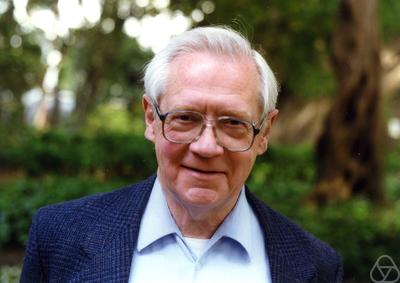
\includegraphics[width=\textwidth]{images/ogg.jpg}}
	\caption{Andrew Ogg}
	\end{subfigure} \hspace{0.05cm}
	%
	\begin{subfigure}{0.3\textwidth}
	\captionsetup{labelformat=empty}
	\centering
	\fbox{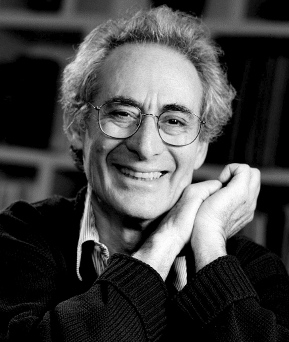
\includegraphics[width=0.83\textwidth]{images/mazur.jpg}}
	\caption{Barry Mazur}
	\end{subfigure}
	\end{figure}
\end{frame}



% Quadratic Rational EC
\begin{frame}[plain]
\footnotesize
\begin{thm}[Najman, 2015]
Let $E/\Q$ be a rational elliptic curve, and let $K/\Q$ be a quadratic number field. Then the possible torsion subgroups $E(K)_\tors$ are precisely:
	\[
	\begin{cases}
	\Z/n\Z, & \text{with } n= 1, 2, \ldots, 10, 12, 15, 16 \text{ or} \\
	\Z/2\Z \oplus \Z/2n\Z, & \text{with } n= 1, 2, \ldots, 6 \text{ or} \\
	\Z/3\Z \oplus \Z/3n\Z, & \text{with } n= 1, 2 \text{ or} \\
	\Z/4\Z \oplus \Z/4\Z
	\end{cases}
	\]
Each such possibility occurs for infinitely many elliptic curves except for $\Z/15\Z$, which occurs only for the elliptic curves \texttt{50b1} and \texttt{50a3} over $\Q(\sqrt{5})$ and the elliptic curves \texttt{50b2} and \texttt{450b4} over $\Q(\sqrt{-15})$. 
\end{thm}
	\begin{figure}[!ht]
	\centering
	\captionsetup{labelformat=empty}
	\fbox{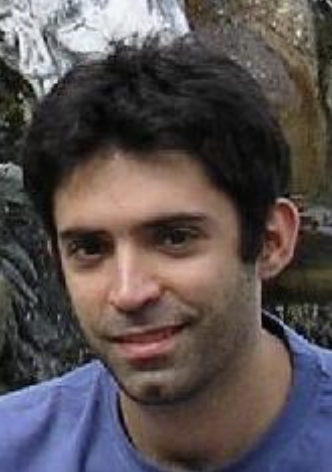
\includegraphics[width=0.18\textwidth]{images/najman2.png}}
	\caption{Filip Najman}
	\end{figure}
\end{frame}



% Cubic Rational EC
\begin{frame}[plain]
\begin{thm}[Najman, 2015]
Let $E/\Q$ be a rational elliptic curve, and let $K/\Q$ be a cubic number field. Then the possible torsion subgroups $E(K)_\tors$ are precisely:
	\[
	\begin{cases}
	\Z/n\Z, & \text{with } n= 1, 2, \ldots, 10, 12, 13, 14, 18, 21 \text{ or} \\
	\Z/2\Z \oplus \Z/2n\Z, & \text{with } n= 1, 2, 3, 4, 7
	\end{cases}
	\]
Each such possibility occurs for infinitely many elliptic curves except for $\Z/21\Z$, which only occurs for the elliptic curve \texttt{162b1} over $\Q(\zeta_9)^+$.
\end{thm}
	\begin{figure}[!ht]
	\centering
	\captionsetup{labelformat=empty}
	\fbox{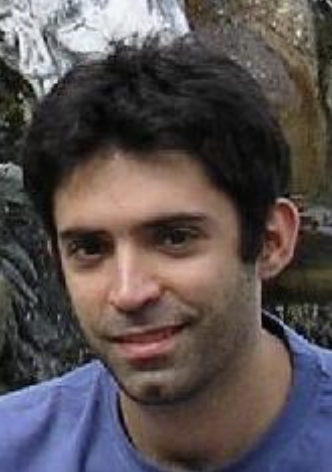
\includegraphics[width=0.18\textwidth]{images/najman2.png}}
	\caption{Filip Najman}
	\end{figure}
\end{frame}



% Quartic Rational EC
\begin{frame}[plain]
\footnotesize
\begin{thm}[Chou, 2015; Gonz\'alez-Jimenez, Lozano-Robledo, 2016; Gonz\'alez-Jimenez, Najman, 2016]
Let $E/\Q$ be a rational elliptic curve, and let $K/\Q$ be a quartic number field. Then the possible torsion subgroups $E(K)_\tors$ are precisely:
	\[
	\begin{cases}
	\Z/n\Z, & \text{with } n= 1, 2, \ldots, 10, 12, 13, 15, 16, 20, 24 \text{ or} \\
	\Z/2\Z \oplus \Z/2n\Z, & \text{with } n= 1, 2, \ldots, 6, 8 \text{ or} \\
	\Z/3\Z \oplus \Z/3n\Z, & \text{with } n= 1, 2 \text{ or} \\
	\Z/4\Z \oplus \Z/4n\Z, & \text{with } n= 1, 2 \text{ or} \\
	\Z/5\Z \oplus \Z/5\Z, & \text{or} \\
	\Z/6\Z \oplus \Z/6\Z 
	\end{cases}
	\]
Each such possibility occurs for infinitely many elliptic curves except for $\Z/15\Z$, which occurs only for the elliptic curves with $j(E) \in \{ -5^2/2, -5^2 \cdot 241^3/2^3$, $-5 \cdot 29^3/2^5, 5 \cdot 211^3/2^{15} \}$ over some quartic field. 
\end{thm}
	\begin{figure}[h]
	\centering
	\begin{subfigure}{0.20\textwidth}
	\captionsetup{labelformat=empty}
	\centering
	\fbox{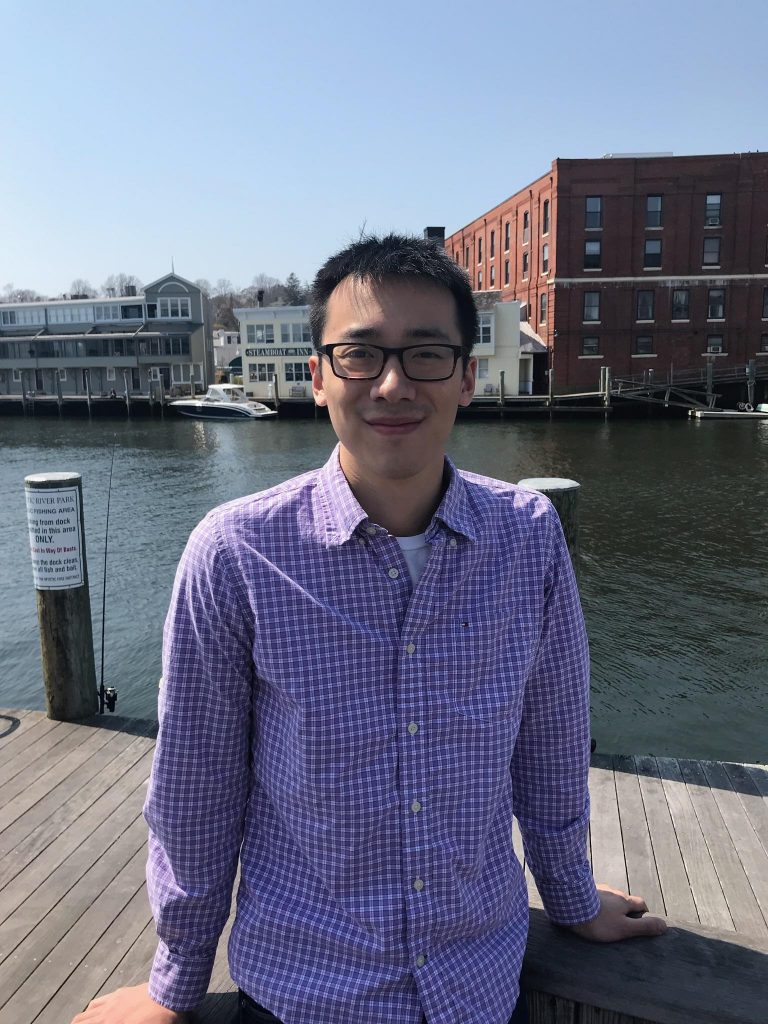
\includegraphics[width=0.62\textwidth]{images/chou.jpg}}
	\caption{\tiny Michael Chou}
	\end{subfigure} \quad
	%
	\begin{subfigure}{0.20\textwidth}
	\captionsetup{labelformat=empty}
	\centering
	\fbox{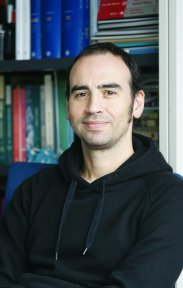
\includegraphics[width=0.45\textwidth]{images/jimenez2.jpeg}}
	\caption{\tiny \hspace{0.7cm}Enrique \\ \;\;\;Gonz\'alez-Jim\'enez}
	\end{subfigure}
	%
	\begin{subfigure}{0.20\textwidth}
	\captionsetup{labelformat=empty}
	\centering
	\fbox{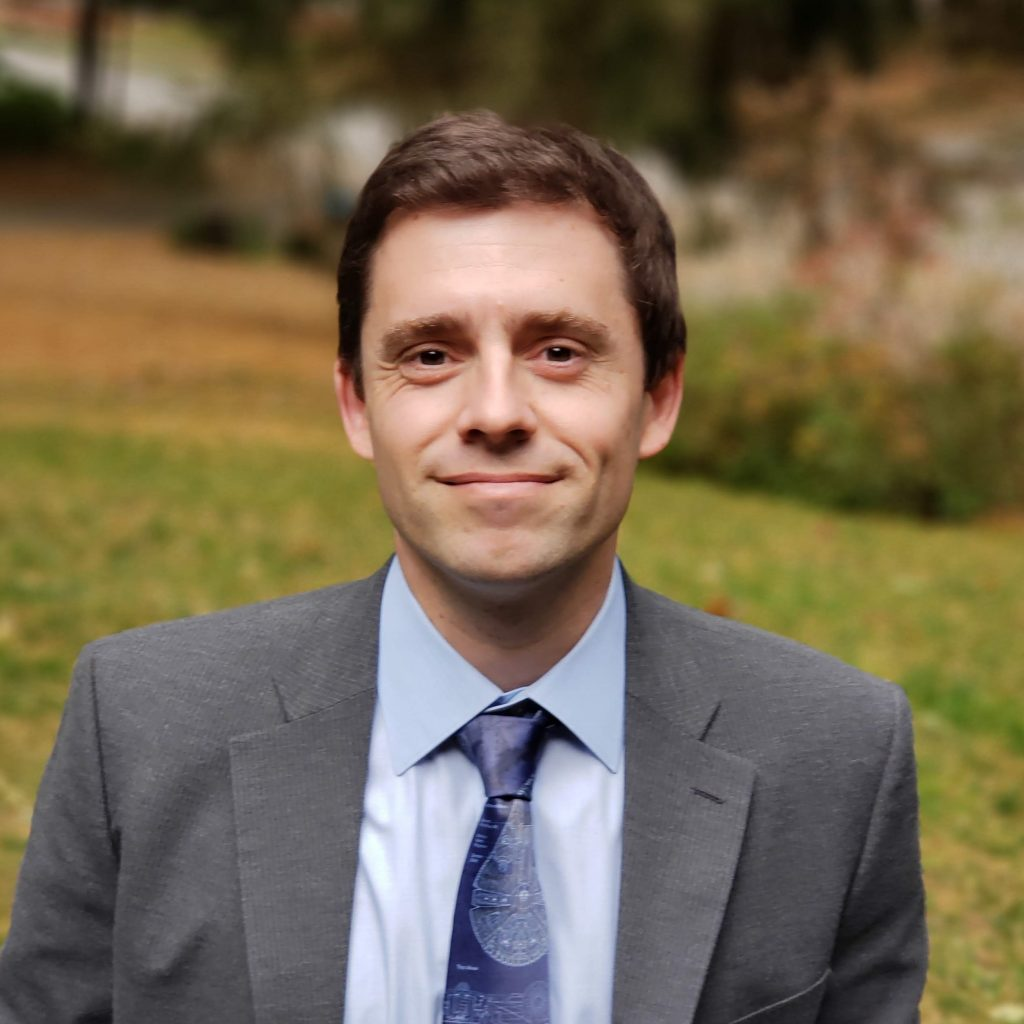
\includegraphics[width=0.72\textwidth]{images/robledo.jpg}}
	\caption{\tiny \hspace{0.7cm}\'Alvaro \\ \;\;\;\;\;Lozano-Robledo}
	\end{subfigure} \quad
	%
	\begin{subfigure}{0.20\textwidth}
	\captionsetup{labelformat=empty}
	\centering
	\fbox{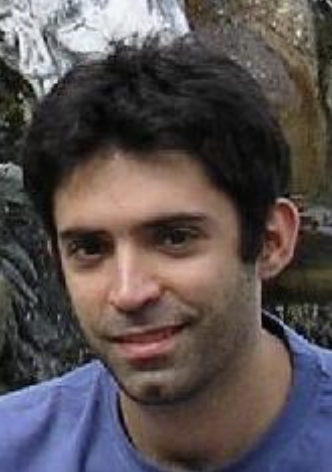
\includegraphics[width=0.58\textwidth]{images/najman2.png}}
	\caption{\tiny Filip Najman}
	\end{subfigure}
	\end{figure}
\end{frame}



% Quintic Rational EC
\begin{frame}[plain]
\begin{thm}[Gonz\'alez-Jimenez, 2016]
Let $E/\Q$ be a rational elliptic curve, and let $K/\Q$ be a quintic number field. Then the possible torsion subgroups $E(K)_\tors$ are precisely:
	\[
	\begin{cases}
	\Z/n\Z, & \text{with } n= 1, 2, \ldots, 12, 25 \text{ or} \\
	\Z/2\Z \oplus \Z/2n\Z, & \text{with } n= 1, 2, 3, 4
	\end{cases}
	\]
Each of these possibilities occurs infinitely many times except for $\Z/11\Z$ which occurs for the elliptic curves \texttt{121a2}, \texttt{121c2}, and \texttt{121b1} over some quintic field. 
\end{thm}
	\begin{figure}[!ht]
	\centering
	\captionsetup{labelformat=empty}
	\fbox{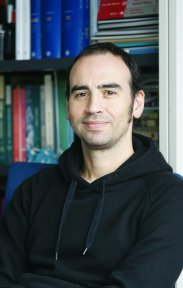
\includegraphics[width=0.18\textwidth]{images/jimenez2.jpeg}}
	\caption{Enrique Gonz\'alez-Jim\'enez}
	\end{figure}
\end{frame}



% Sextic Rational EC
\begin{frame}[plain]
\footnotesize
\begin{thm}[Daniels, Gonz\'alez-Jimenez, 2018; Gu{\u{z}}vi\'c, 2019]
Let $E/\Q$ be a rational elliptic curve, and let $K/\Q$ be a sextic number field. Then the possible torsion subgroups $E(K)_\tors$ are among:
	\[
	\begin{cases}
	\Z/n\Z, & \text{with } n= 1, 2, \ldots, 16, 18, 21, 30, n \neq 11  \text{ or} \\
	\Z/2\Z \oplus \Z/2n\Z, & \text{with } n= 1, 2, \ldots, 7, 9 \text{ or} \\
	\Z/3\Z \oplus \Z/3n\Z, & \text{with } n= 1, 2, 3, 4, 6^* \text{ or} \\
	\Z/4\Z \oplus \Z/4n\Z, & \text{with } n= 1, 3 \\
	\Z/6\Z \oplus \Z/6\Z 
	\end{cases}
	\]
Each such possibility occurs for infinitely many elliptic curves except for $\Z/15\Z$, $\Z/21\Z$, $\Z/30\Z$, $\Z/4\Z \oplus \Z/12\Z$, and possibly $\Z/3\Z \oplus \Z/18\Z$. 
\end{thm}
	\begin{figure}[h]
	\centering
	\begin{subfigure}{0.30\textwidth}
	\captionsetup{labelformat=empty}
	\centering
	\fbox{
\includegraphics[width=0.63\textwidth]{images/daniels.jpeg}}
	\caption{\tiny Harris Daniels}
	\end{subfigure} 
	%
	\begin{subfigure}{0.30\textwidth}
	\captionsetup{labelformat=empty}
	\centering
	\fbox{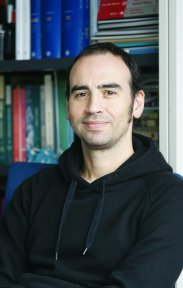
\includegraphics[width=0.40\textwidth]{images/jimenez2.jpeg}}
	\caption{\tiny Enrique Gonz\'alez-Jim\'enez}
	\end{subfigure}
	%
	\begin{subfigure}{0.30\textwidth}
	\captionsetup{labelformat=empty}
	\centering
	\fbox{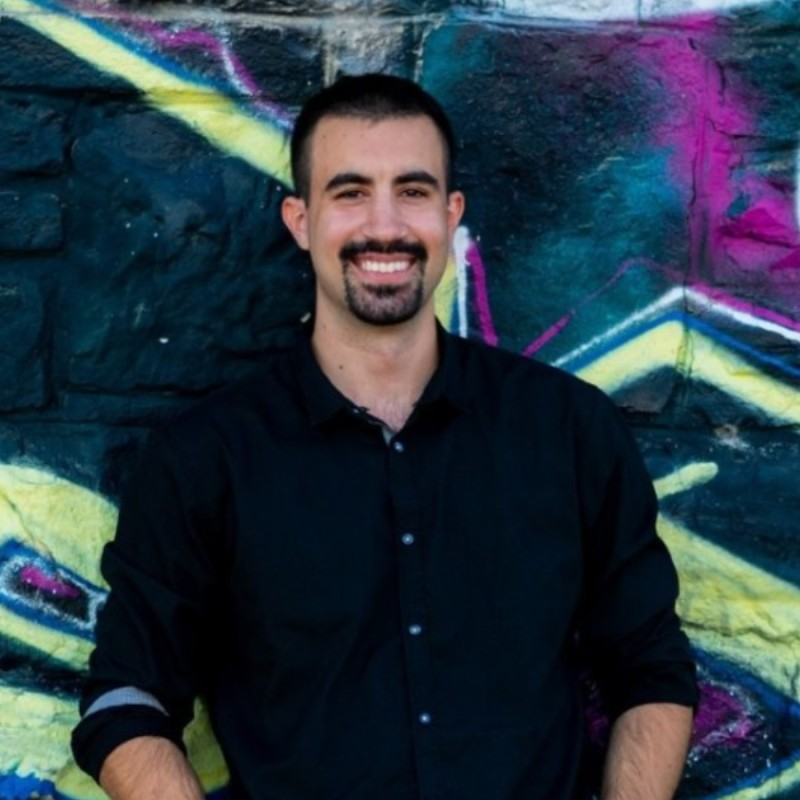
\includegraphics[width=0.635\textwidth]{images/tomislav.jpeg}}
	\caption{\tiny Tomislav Gu{\u{z}}vi\'c}
	\end{subfigure}
	\end{figure}
\end{frame}



% Other Fields Rational EC
\begin{frame}[plain]
\begin{thm}[Gonz\'alez-Jimenez, Najman, 2016]
Let $E/\Q$ be a rational elliptic curve, and let $K/\Q$ be a number field whose smallest prime divisor is at least 7, then the only possible torsion subgroups $E(\Q)_\tors$ are those from Mazur's list, namely:
	\[
	\begin{cases}
	\Z/n\Z, & \text{with } n= 1, 2, \ldots, 10, 12 \text{ or} \\
	\Z/2\Z \oplus \Z/2n\Z, & \text{with } n= 1, 2, 3, 4
	\end{cases}
	\]
Each such possibility occurs for infinitely many elliptic curves. In fact, if the largest prime divisor is at least 11, then $E(K)_\tors=$ $E(\Q)_\tors$. 
\end{thm}
	\begin{figure}[h]
	\centering
	\begin{subfigure}{0.40\textwidth}
	\captionsetup{labelformat=empty}
	\centering
	\fbox{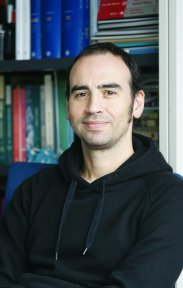
\includegraphics[width=0.40\textwidth]{images/jimenez2.jpeg}}
	\caption{\footnotesize \hspace{0.4cm} Enrique Gonz\'alez-Jim\'enez}
	\end{subfigure}
	%
	\begin{subfigure}{0.40\textwidth}
	\captionsetup{labelformat=empty}
	\centering
	\fbox{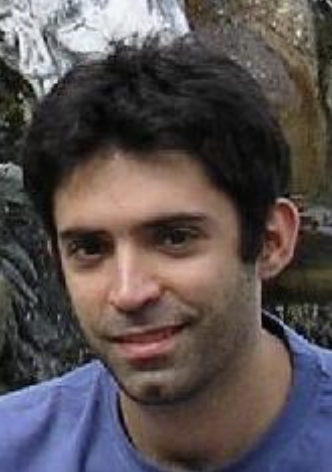
\includegraphics[width=0.45\textwidth]{images/najman2.png}}
	\caption{\footnotesize Filip Najman}
	\end{subfigure}
	\end{figure}
\end{frame}



% Research
% !TEX root = ../swarthmore_talk.tex

% Odd Degree Galois
\begin{frame}[plain]
\ctext{Classification over Odd Degree Galois Fields}
\end{frame}



% Odd Degree Galois Classification
\begin{frame}[plain,c]
\begin{thm}[M.]
The set $\Phi_\Q^{\Gal,\text{odd}}(d^\infty)$ is finite, and if $E(K)_\tors \in \Phi_\Q^{\Gal,\text{odd}}(d^\infty)$, then $E(K)_\tors$ is precisely one of the following:
	\[
	\begin{cases}
	\Z/n\Z, & n= 1, 2, \ldots, 14, 18, 19, 21, 25, 27, 43, 67, 163 \text{ or} \\
	\Z/2\Z \oplus \Z/2n\Z, & n= 1, 2, 3, 4, 7.
	\end{cases}
	\]
Moreover, each such possibility occurs. 
\end{thm}
	\[
	\Phi_\Q^{\Gal,\text{odd}}(d^\infty):= \bigcup_{\substack{d \in \N \\ d \text{ odd}}} \Phi_\Q^{\Gal}(d)
	\]
\end{frame}



% Odd Degree Galois by Degree Table
\begin{frame}[plain,c]
        \begin{table}[!ht]
        \centering
        \resizebox{0.72\textwidth}{!}{%
        \begin{tabular}{>{\raggedright\arraybackslash}p{2.4cm}|%
           >{\centering\arraybackslash}p{5cm}||%
           >{\raggedright\arraybackslash}p{2.6cm}|%
           >{\centering\arraybackslash}p{5cm}%
          } \hline
        $F(d)^+$ & $\Phi_\Q^{\Gal}(d)$ & $F(d)^+$ & $\Phi_\Q^{\Gal}(d)$  \\ \hline
        & & & \\ %
        $(0,0,0^+,0^+)$ & $\Phi(1)$ & $(2,0,1^+,1^+)$ & $\Phi_\Q(3) \cup \{ \Z/19\Z, \Z/27\Z,$ $\Z/43\Z, \Z/67\Z \}$ \\
        & & & \\ %
        $(0,1,0^+,0^+)$ & $\Phi_\Q(5)$ & $(2,1^+,0,0)$ & $\Phi_\Q(3) \cup \Phi_\Q(5) \cup \{ \Z/19\Z, \Z/27\Z \}$ \\
        & & & \\ %
        $(1,0,0,0)$ & $\Phi_\Q(3)$ & $(2,1^+,0,1^+)$ & $\Phi_\Q(3) \cup \Phi_\Q(5) \cup \{ \Z/19\Z, \Z/27\Z, \Z/67\Z \}$ \\
        & & & \\ %
        $(1,0,0,1^+)$ & $\Phi_\Q(3) \cup \{ \Z/11\Z \}$ & $(2,1^+,1^+,0)$ & $\Phi_\Q(3) \cup \Phi_\Q(5) \cup \{ \Z/19\Z, \Z/27\Z, \Z/43\Z \}$ \\
        & & & \\ %
        $(1,0,1^+,0)$ & $\Phi_\Q(3) \cup \{ \Z/43\Z \}$ & $(2,1^+,1^+,1^+)$ & $\Phi_\Q(3) \cup \Phi_\Q(5) \cup \{ \Z/19\Z, \Z/27\Z, \Z/43\Z,$ $\Z/67\Z \}$ \\
        & & & \\ %
        $(1,0,1^+,1^+)$ & $\Phi_\Q(3) \cup \{ \Z/11\Z, \Z/43\Z \}$ & $(4^+,0,0,0)$ & $\Phi_\Q(3) \cup \{ \Z/19\Z, \Z/27\Z,$ $\Z/163\Z \}$ \\
        & & & \\ %
        $(1,1^+,0,0)$ & $\Phi_\Q(3) \cup \Phi_\Q(5)$ & $(4,0,0,1^+)$ & $\Phi_\Q(3) \cup \{ \Z/19\Z, \Z/27\Z,$ $\Z/67\Z, \Z/163\Z \}$ \\
        & & & \\ %
        $(1,1^+,0,1^+)$ & $\Phi_\Q(3) \cup \Phi_\Q(5) \cup \{ \Z/67\Z \}$ & $(4,0,1^+,0)$ & $\Phi_\Q(3) \cup \{ \Z/19\Z, \Z/27\Z,$ $\Z/47\Z, \Z/163\Z \}$ \\
        & & & \\ %
        $(1,1^+,1^+,0)$ & $\Phi_\Q(3) \cup \Phi_\Q(5) \cup \{ \Z/43\Z \}$ & $(4,0,1^+,1^+)$ & $\Phi_\Q(3) \cup \{ \Z/19\Z, \Z/27\Z,$ $\Z/43\Z, \Z/67\Z, \Z/163\Z \}$ \\
        & & & \\ %
        $(1,1^+,1^+,1^+)$ & $\Phi_\Q(3) \cup \Phi_\Q(5) \cup \{ \Z/43\Z,$ $\Z/67\Z \}$ & $(4,1^+,0,0)$ & $\Phi_\Q(3) \cup \Phi_\Q(5) \cup \{ \Z/19\Z, \Z/27\Z, \Z/163\Z \}$ \\
        & & & \\ %
        $(2,0,0,0)$ & $\Phi_\Q(3) \cup \{ \Z/19\Z, \Z/27\Z \}$ & $(4,1^+,0,1^+)$ & $\Phi_\Q(3) \cup \Phi_\Q(5) \cup \{ \Z/19\Z,$ $\Z/27\Z, \Z/67\Z, \Z/163\Z \}$ \\
        & & & \\ %
        $(2,0,0,1^+)$ & $\Phi_\Q(3) \cup \{ \Z/19\Z, \Z/27\Z,$ $\Z/67\Z \}$ & $(4,1^+,1^+,0)$ & $\Phi_\Q(3) \cup \Phi_\Q(5) \cup \{ \Z/19\Z,$ $\Z/27\Z, \Z/43\Z, \Z/163\Z \}$ \\
        & & & \\ %
        $(2,0,1^+,0)$ & $\Phi_\Q(3) \cup \{ \Z/19\Z, \Z/27\Z,$ $\Z/43\Z \}$ & $(4^+,1^+,1^+,1^+)$ & $\Phi_\Q(3) \cup \Phi(5) \cup \{ \Z/19\Z,$ $\Z/27\Z, \Z/43\Z, \Z/67\Z, \Z/163\Z \}$
        \end{tabular}%
        }
        \end{table}
\end{frame}















% Nonic Galois Field
\begin{frame}[plain]
\ctext{Classification over Nonic Galois Fields}
\end{frame}



% Quartic Galois Rational EC
\begin{frame}[plain]
\small
\begin{thm}[Chou, 2015]
Let $E/\Q$ be a rational elliptic curve, and let $K/\Q$ be a quartic Galois number field. Then the possible torsion subgroups $E(K)_\tors$ are precisely:
	\[
	\begin{cases}
	\Z/n\Z, & \text{with } n= 1, 2, \ldots, 10, 12, 13, 15, 16 \text{ or} \\
	\Z/2\Z \oplus \Z/2n\Z, & \text{with } n= 1, 2, \ldots, 6, 8 \text{ or} \\
	\Z/3\Z \oplus \Z/3n\Z, & \text{with } n= 1, 2 \text{ or} \\
	\Z/4\Z \oplus \Z/4n\Z, & \text{with } n= 1, 2 \text{ or} \\
	\Z/5\Z \oplus \Z/5\Z, & \text{or} \\
	\Z/6\Z \oplus \Z/6\Z.
	\end{cases}
	\]
\end{thm}
	\begin{figure}[!ht]
	\centering
	\captionsetup{labelformat=empty}
	\fbox{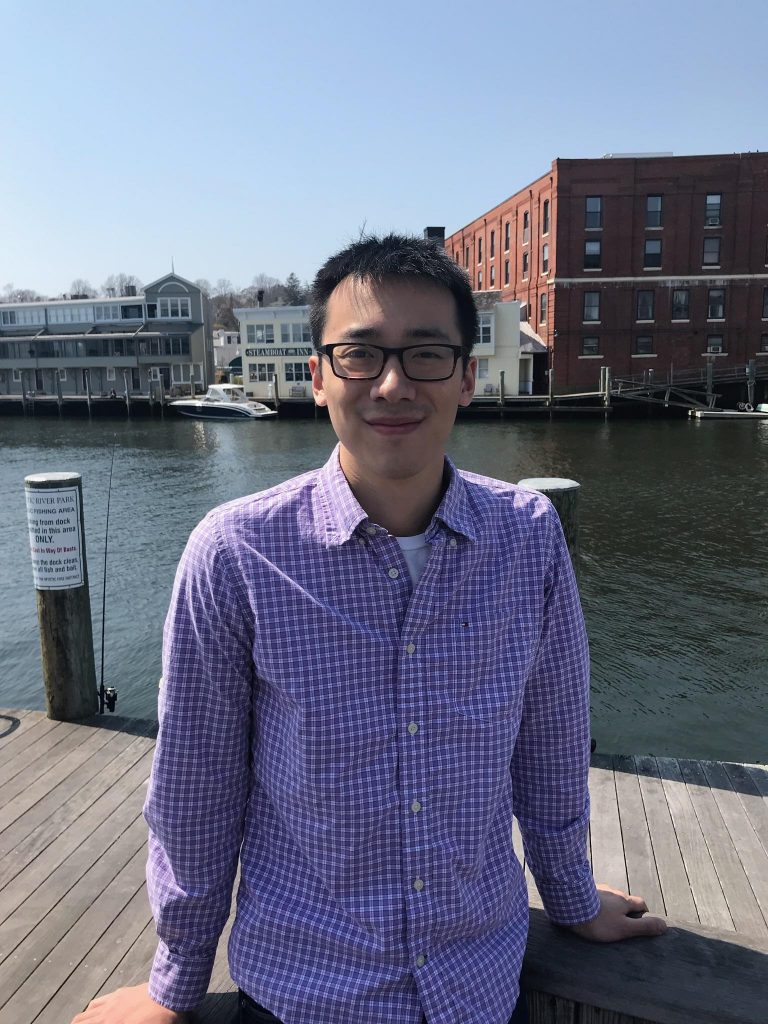
\includegraphics[width=0.20\textwidth]{images/chou.jpg}}
	\caption{Michael Chou}
	\end{figure}
\end{frame}



% Outline
\begin{frame}[plain]
\frametitle{Outline of the Classification}
        \begin{enumerate}
        \item Determine the possible prime orders. \vfill
        \item Bound the $p$-Sylow Subgroups. \vfill
        \item Create a finite list of possibilities. \vfill
        \item Find examples and eliminate cases. \vfill
        \end{enumerate}
\vfill
\end{frame}



% Step 1. Determine the Possible Prime Orders
\begin{frame}[plain]
\vfill
\begin{center} {\bfseries \Large \textcolor{SwarthGarnet}{Step 1. Determine the Possible Prime Orders}} \end{center}
\vfill 
\end{frame}



% Lozano-Robledo S(d)
\begin{frame}[plain]
\begin{thm}[Lozano-Robledo, 2013]
Let $S_\Q(d)$ be the set of primes such that there exists an elliptic curve $E/\Q$ with a point of order $p$ defined in an extension $K/\Q$ of degree at most $d$. Then $S_\Q(9)= \{ 2, 3, 5, 7, 11, 13, 17, 19 \}$.
\end{thm}
	\begin{figure}[h]
	\centering
	\begin{subfigure}{\textwidth}
	\captionsetup{labelformat=empty}
	\centering
	\fbox{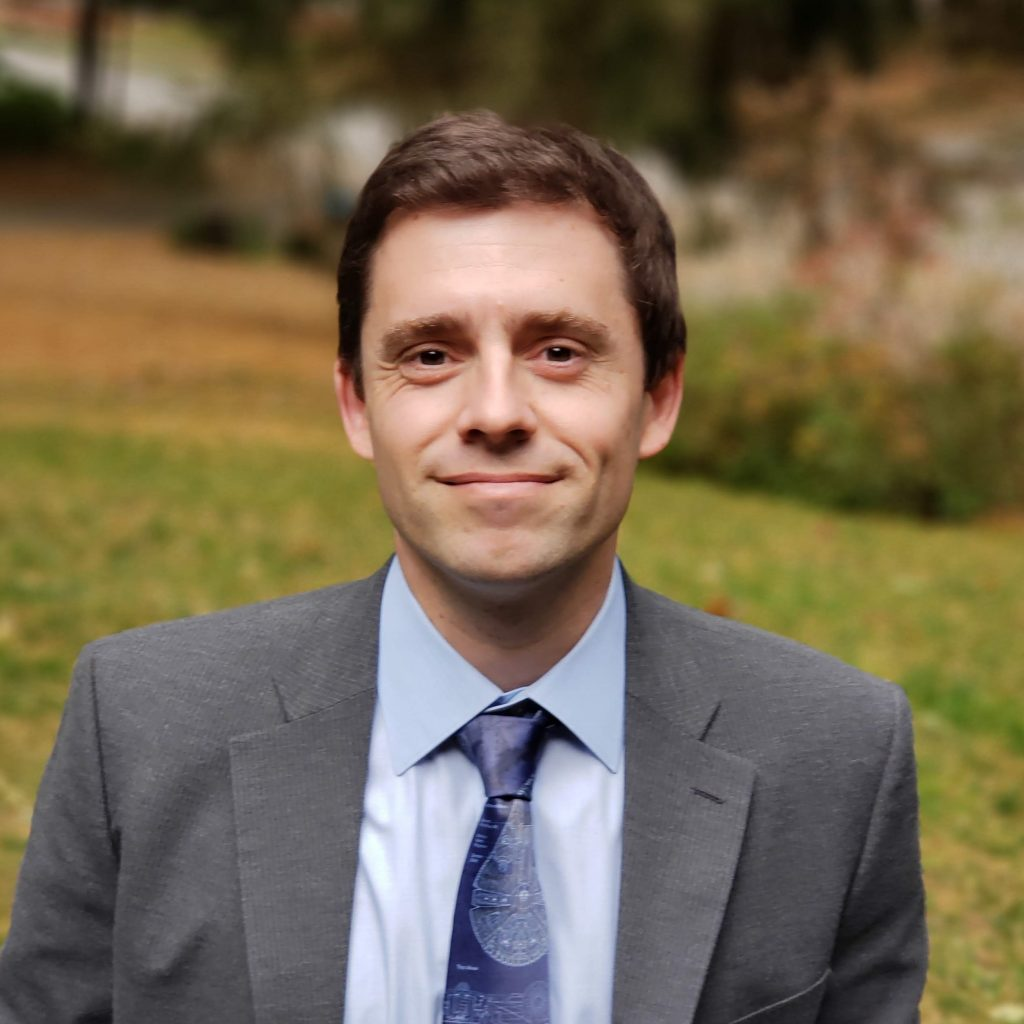
\includegraphics[width=0.2\textwidth]{images/robledo.jpg}}
	\caption{\'Alvaro Lozano-Robledo}
	\end{subfigure}
	\end{figure}

\begin{rem}
Lozano-Robledo computes $S_\Q(d)$ for $1 \leq d \leq 21$ and gives a conjectural formula for $d \geq 1$, which is valid for $1 \leq d \leq 42$, which would follow from a positive answer to Serre's uniformity question. 
\end{rem}
\end{frame}



% Gonzalez-Jimenez, Najman R(d)
\begin{frame}[plain]
\begin{prop}[Gonz\'alez-Jim\'enez, Najman, 2016] \hfill
	\begin{enumerate}[(i)]
	\item $11 \in R_\Q(d)$ if and only if $5 \mid d$.
	\item $17 \in R_\Q(d)$ if and only if $8 \mid d$.
	\end{enumerate}
\end{prop}
	\begin{figure}[h]
	\centering
	\begin{subfigure}{0.35\textwidth}
	\captionsetup{labelformat=empty}
	\centering
	\fbox{\includegraphics[width=0.65\textwidth]{images/jimenez.png}}
	\caption{Enrique Gonz\'alez-Jim\'enez}
	\end{subfigure}
	%
	\begin{subfigure}{0.3\textwidth}
	\captionsetup{labelformat=empty}
	\centering
	\fbox{\includegraphics[width=0.70\textwidth]{images/najman2.png}}
	\caption{Filip Najman}
	\end{subfigure}
	\end{figure}
\end{frame}



% Prime Possible
\begin{frame}[plain]
\begin{prop}
Let $E/\Q$ be a rational elliptic curve, and let $K/\Q$ be a nonic Galois field. If $P \in E(K)$ is a point of prime order $p$, then $p \in \{ 2, 3, 5, 7, 13,$ $19 \}$.
\end{prop}
\end{frame}



% Step 2. Bound the Size of the Sylow Subgroups
\begin{frame}[plain]
\vfill
\begin{center} {\bfseries \Large \textcolor{SwarthGarnet}{Step 2. Bound the Size of the Sylow Subgroups}} \end{center}
\vfill 
\end{frame}



% Full 2-Torsion, Lozano-Robledo
\begin{frame}[plain]
\begin{thm}[Gonz\'alez-Jim\'enez, Lozano-Robledo]
Let $E/\Q$ be an elliptic curve without CM. Let $1 \leq s \leq N$ be fixed integers, and let $T \subseteq E[2^N]$ be a subgroup isomorphic to $\Z/2^s/Z \oplus \Z/2^N \Z$. Then $[\Q(T) \colon \Q]$ is divisible by 2 if $s=N=2$, and otherwise by $2^{2N+2s-8}$ if $N \geq 3$, unless $s \geq 4$ and $j(E)$ is one of the two values:
	\[
	- \dfrac{3 \cdot 18249920^3}{17^{16}}\; \text{ or } - \dfrac{7 \cdot 1723187806080^3}{79^{16}}
	\]
in which case $[\Q(T) \colon \Q]$ is divisible by $3 \cdot 2^{2N+2s-9}$. Moreover, this is best possible in that there are one-parameter families $E_{s,N}(t)$ of elliptic curves over $\Q$ such that for each $s, N \geq 0$ and each $t \in \Q$, and subgroups $T_{s,N} \in E_{s,N}(t)(\ov{\Q})$ isomorphic to $\Z/2^s\Z \oplus \Z/2^N\Z$ such that $[\Q(T_{s,N}) \colon \Q]$ is equal to the bound given above. 
\end{thm}
\end{frame}



% 2-Sylow Bound
\begin{frame}[plain]
\begin{lem}[2-Sylow Bound]
Let $E/\Q$ be a rational elliptic curve, and let $K/\Q$ be a nonic Galois field. Then $E(K)[2^\infty] \subseteq \Z/2\Z \oplus \Z/8\Z$.
\end{lem}
\end{frame}



% Full p-Torsion & Weil-Pairing
\begin{frame}[plain]
\footnotesize
\phantom{.} \vfill
\begin{lem}[Odd Torsion]
Let $K/\Q$ be an odd degree number field, and let $E/\Q$ be a rational elliptic curve. Then $E(K)_\tors$ does not contain full $p$-torsion for all odd primes.
\end{lem}

\pf By the existence of the Weil-pairing, if $E(K)$ contains full $p$-torsion, then $\Q(\zeta_p) \subseteq K$. But for $p > 2$, $[\Q(\zeta_p) \colon \Q]= \phi(p)$ is even, a contradiction. \hfill \qed \vfill
\end{frame}



% Full p-Torsion & Weil-Pairing 2
\begin{frame}[plain]
\footnotesize
\begin{lem}[Galois Isogeny]
Let $K/\Q$ be a Galois extension, and let $E/\Q$ be a rational elliptic curve. If $E(K)[n] \cong \Z/n\Z$, then $E$ has a rational $n$-isogeny. 
\end{lem} \vfill

\begin{lem}[Galois Isogeny]
Let $E/\Q$ be a rational elliptic curve, and let $K/\Q$ be a Galois extension. If $E(K)_\tors \cong \Z/m\Z \oplus \Z/mn\Z$, then $E$ has a rational $n$-isogeny. 
\end{lem} \vfill

\begin{thm}[Fricke, Kenku, Klein, Kubert, Ligozat, Mazur, Ogg, et al.]
Let $N \geq 2$ be such that $X_0(N)$ has a non-cuspidal $\Q$-rational point. Then
	\begin{enumerate}[(i)]
	\item $N \leq 10$ or $N=$ 12, 13, 16, 18, or 25. In this case, $X_0(N)$ is a curve of genus 0, and the $\Q$ rational points on $X_0(N)$ form an infinite 1-parameter family, or
	\item $N=$ 11, 14, 15, 17, 19, 21, or 27, i.e. $X_0(N)$ is a rational elliptic curve (in each case $X_0(N)(\Q)$ is finite, or
	\item $N=$ 37, 43, 67, or 163. In this case, $X_0(N)$ is a curve of genus $\geq 2$ and by Faltings' Theorem has only finitely many $\Q$-rational points. 
	\end{enumerate}
In particular, a rational elliptic curve may only have a rational cyclic $n$-isogeny for $n \leq 19$ or $n \in \{ 21, 25, 27, 37, 43, 67,163\}$. Furthermore, if $E$ does not have CM, then $n \leq 18$ or $n \in \{ 21, 25, 37 \}$.
\end{thm}
\end{frame}



% Sylow Bounds
\begin{frame}[plain]
\footnotesize
\begin{lem}[$p$-Sylow bounds]
Let $E/\Q$ be a rational elliptic curve, and let $K/\Q$ be a nonic Galois field. Then
	\[
	\begin{aligned}
	E(K)[2^\infty]&\subseteq \Z/2\Z \oplus \Z/8\Z \\
	E(K)[3^\infty]&\subseteq \Z/27\Z \\
	E(K)[5^\infty]&\subseteq \Z/25\Z \\
	E(K)[7^\infty]&\subseteq \Z/7\Z \\
	E(K)[13^\infty]&\subseteq \Z/13\Z \\
	E(K)[19^\infty]&\subseteq \Z/19\Z
	\end{aligned}
	\]
\end{lem}
\end{frame}



% Step 3. Create a Finite List of Possibilities
\begin{frame}[plain]
\vfill
\begin{center} {\bfseries \Large \textcolor{SwarthGarnet}{Step 3. Create a Finite List of Possibilities}} \end{center}
\vfill 
\end{frame}



% Finite List
\begin{frame}[plain]
\footnotesize
\begin{lem}
Let $E/\Q$ be a rational elliptic curve, and let $K/\Q$ be a nonic Galois field. Then $E(K)_\tors$ is isomorphic to one of the following (although not all cases need occur):
	\[
	\begin{cases}
	\Z/n\Z, & n= 1, 2, \ldots, 10, 12, 13, 14, 15, 18, 19, 21, 25, 27 \\
	\Z/2\Z \oplus \Z/2n\Z, & n= 1, 2, \ldots, 7, 9, 10, 12, 13, 14, 15, 18, 19, 21, 25, 27
	\end{cases}
	\]
\end{lem} 
\end{frame}



% Step 4. Find Examples \& Eliminate Cases
\begin{frame}[plain]
\vfill
\begin{center} {\bfseries \Large \textcolor{SwarthGarnet}{Step 4. Find Examples \& Eliminate Cases}} \end{center}
\vfill 
\end{frame}



% Upstairs/Downstairs Games
\begin{frame}[plain] \frametitle{}
	\vspace{1cm} \vfill 
	
	\begin{center}
	{\color{SwarthGarnet}\Large\bfseries Upstairs/Downstairs Games}
	\end{center}
	
	\begin{figure}[h,t]
	\centering
	\begin{subfigure}{\textwidth}
	\captionsetup{labelformat=empty}
	\centering
	\fbox{\includegraphics[width=0.6\textwidth]{images/escher.png}}
	\caption{M.C. Escher's Relativity}
	\end{subfigure}
	\end{figure}
\end{frame}



% Base Extension
\begin{frame}[plain]
\begin{prop}
Let $E/\Q$ be a rational elliptic curve, and let $F/\Q$ be a cubic Galois field. Then there exists a nonic Galois field $K$ such that $E(K)_\tors \cong E(F)_\tors$.
\end{prop}

\pf 
\begin{itemize}
\item If $F_1, F_2$ are distinct cubic Galois fields, then $F_1F_2$ is a nonic Galois extension. It suffices to prove there are infinitely many distinct cubic Galois fields. 
\item For a chosen integer $k$, define $a:= k^2 + k + 7$.
\item The field $K_a:= \Q(x^3 - ax + a)$ is a cubic Galois field. For each distinct $a$, the fields $K_a$ are distinct. \hfill\qed
\end{itemize}

\begin{cor}
$\Phi_\Q^{\Gal}(3) \subseteq \Phi_\Q^{\Gal}(9)$
\end{cor}
\end{frame}



% Examples of Torsion Subgroups
\begin{frame}[plain]
	\begin{table}[!ht]
	\centering
	\caption{Examples of torsion subgroups $\Phi_\Q(3) \setminus \Phi(1)$.\label{tab:3qsm1}}
	\begin{tabular}{ccc} \hline
	Torsion Subgroup & Elliptic Curve & Galois Cubic Field \\ \hline
	$\Z/13\Z$ & \ofsbo{} & \qzetasp{} \\
	$\Z/14\Z$ & \fnat{} & \qzetasp{} \\
	$\Z/18\Z$ & \ofaf{} & \qzetasp{} \\
	$\Z/21\Z$ & \ostbo{} & \qzetanp{} \\
	$\Z/2\Z \times \Z/14\Z$ & \onttco{} & \ttnsoo{}
	\end{tabular}
	\end{table}

        \begin{table}[!ht]
        \centering
        \caption{Examples of $E(K)$ with 19 and 27-torsion over nonic fields.\label{tab:1927tor}}
        \begin{tabular}{cccc} \hline
        $E(K)_\tors$ & $E(\Q)_\tors$ &  $E$ & $K$ \\ \hline
        $\Z/19\Z$ & $\{ \O \}$ & \tsoao{} & \qzetantp{} \\ 
        $\Z/27\Z$ & $\Z/3\Z$ & \tsaf{} & \qzetatsp{}
        \end{tabular}
        \end{table}
\end{frame}



% Remaining Groups
\begin{frame}[plain]
This leaves the following list of torsion subgroups whose existence or non-existence we have yet to prove. \pspace
	\[
	\begin{cases}
	\Z/n\Z, & n= 15, 25 \\
	\Z/2\Z \oplus \Z/2n\Z, & n= 5, 6, 9, 10, 12, 13, 14, 15, 18, 19, 21, 25, 27
	\end{cases}
	\]
\end{frame}



% Najman Growth Lemmas
\begin{frame}[plain]
\begin{lem}[Najman, 2015]
Let $p, q$ be distinct odd primes, $F_2/F_1$ a Galois extension of number fields such that $\Gal(F_2/F_1) \simeq \Z/q\Z$ and $E/F_1$ an elliptic curve with no $p$-torsion over $F_1$. Then if $q$ does not divide $p-1$ and $\Q(\zeta_p) \not\subset F_2$, then $E(F_2)[p]=0$. 
\end{lem}

\begin{lem}[Najman, 2015]
Let $p$ be an odd prime number, $q$ a prime not dividing $p$, $F_2/F_1$ a Galois extension of number fields such that $\Gal(F_2/F_1) \simeq \Z/q\Z$, $E/F_1$ an elliptic curve, and suppose $E(F_1) \supset \Z/p\Z$, $E(F_1) \not\supset \Z/p^2\Z$, and $\zeta_p \notin F_2$. Then $E(F_2) \not\supset \Z/p^2\Z$.
\end{lem} 
\end{frame}



% Field of Definition Degree
\begin{frame}[plain]
\begin{prop}
Let $E/\Q$ be a rational elliptic curve, and let $K/\Q$ be a nonic Galois field. Suppose $P \in E(K)_\tors$ is a point of order $p$. Then
        \begin{enumerate}[(i)]
        \item if $p \in \{ 3, 5 \}$, then $P$ is defined over $\Q$, i.e. $P \in E(\Q)[p]$.
        \item if $p= 13$, then there is a cubic field $F \subseteq K$ with $P \in E(F)[p]$. 
        \item if $p \in \{ 2, 7 \}$, then $P$ is defined over $\Q$, i.e. $P \in E(\Q)[p]$, or there is a cubic field $F \subseteq K$ with $P \in E(F)[p]$. 
        \end{enumerate}
\end{prop}
\end{frame}



% Z/2Z x Z/10Z
\begin{frame}[plain]
\footnotesize
\begin{lem}
Let $E/\Q$ be a rational elliptic curve, and let $K/\Q$ be a nonic Galois field. Then $E(K)_\tors$ does not contain $\Z/2\Z \oplus \Z/10\Z$.
\end{lem} \pspace

\pf
\begin{itemize}
\item By our previous result, we know that $E(K)[5^\infty]= E(\Q)[5^\infty] \cong \Z/5\Z$. 
\item Choosing a model $E: y^2= x^3 + Ax + B$, we know the $x$-coordinates of points of order 2 correspond to roots of $x^3 + Ax + B$. 
\item As $E(K)_\tors \supseteq \Z/2\Z \oplus \Z/2\Z$, $K$ contains a splitting field for $x^3 + Ax + B$, which has degree 1, 3, or 6. 
\item Degree 6 is not possible as $K/\Q$ has odd degree. Then $\Q(E(K)[2^\infty])$ is defined over at most a cubic field. 
\item But then either $E(\Q)_\tors \cong \Z/2\Z \oplus \Z/10\Z$ or there is a cubic field, $F$, with $E(F)_\tors \cong \Z/2\Z \oplus \Z/10\Z$, contradicting the classification of either $\Phi(1)$ or $\Phi_\Q(3)$. \hfill\qed
\end{itemize}
\end{frame}



% Nonic Galois Result
\begin{frame}[plain]
\begin{thm}[M.]
Let $E/\Q$ be a rational elliptic curve, and let $K/\Q$ be a nonic Galois field. Then $E(K)_\tors$ is isomorphic to precisely one of the following:
	\[
	\begin{cases}
	\Z/n\Z, & n= 1, 2, \ldots, 10, 12, 13, 14, 18, 19, 21, 27 \\
	\Z/2\Z \oplus \Z/2n\Z, & n= 1, 2, 3, 4, 7
	\end{cases}
	\]
\end{thm}
\end{frame}



% Nonic Galois Examples
\begin{frame}[plain]
	\begin{table}[!ht]
	\centering
	\caption{Examples of each possible $E(K)_\tors$ in $\Phi_\Q^{\Gal}(9)$.}
	\resizebox{!}{0.36\textwidth}{%
	\begin{tabular}{cccc} \hline
	 $E(K)_\tors$ & Cremona Label & $E(\Q)_\tors$ & $K$ \\ \hline
	$\{ \O \}$ & \ooat{} & $\{ \O \}$ & \qzetantp{} \\
	$\Z/2\Z$ & \ffafiv{} & $\Z/2\Z$ & \qzetantp{} \\
	$\Z/3\Z$ & \onao{} & $\Z/3\Z$ & \qzetantp{} \\
	$\Z/4\Z$ & \ofas{} & $\Z/4\Z$ & \qzetantp{} \\
	$\Z/5\Z$ & \ooao{} & $\Z/5\Z$ & \qzetantp{} \\
	$\Z/6\Z$ & \ofat{} & $\Z/6\Z$ & \qzetantp{} \\
	$\Z/7\Z$ & \tsbo{} & $\Z/7\Z$ & \qzetantp{} \\
	$\Z/8\Z$ & \ffafo{} & $\Z/8\Z$ & \qzetantp{} \\
	$\Z/9\Z$ & \ffbt{} & $\Z/9\Z$ & \qzetantp{} \\
	$\Z/10\Z$ & \ssco{} & $\Z/10\Z$ & \qzetantp{} \\
	$\Z/12\Z$ & \nzct{} & $\Z/12\Z$ & \qzetantp{} \\
	$\Z/13\Z$ & \ofsbo{} & $\{ \O \}$ & \qzetantp{} \\
	$\Z/14\Z$ & \fnaf{} & $\Z/2\Z$ & \qzetantp{} \\
	$\Z/18\Z$ & \tszsozot{} & $\Z/6\Z$ & \nnezsb{} \\
	$\Z/19\Z$ & \tsoao{} & $\{ \O \}$ & \qzetantp{} \\
	$\Z/21\Z$ & \ostbo{} & $\Z/3\Z$ & \nnstfttf{} \\
	$\Z/27\Z$ & \tsaf{} & $\Z/3\Z$ & \qzetatsp{} \\
	$\Z/2\Z \oplus \Z/2\Z$ & \ffat{} & $\Z/2\Z \oplus \Z/2\Z$ & \qzetantp{} \\
	$\Z/2\Z \oplus \Z/4\Z$ & \ffao{} & $\Z/2\Z \oplus \Z/4\Z$ & \qzetantp{} \\
	$\Z/2\Z \oplus \Z/6\Z$ & \tzat{} & $\Z/2\Z \oplus \Z/6\Z$ & \qzetantp{} \\
	$\Z/2\Z \oplus \Z/8\Z$ & \tozet{} & $\Z/2\Z \oplus \Z/8\Z$ & \qzetantp{} \\
	$\Z/2\Z \oplus \Z/14\Z$ & \onttco{} & $\{ \O \}$ & \nnstfttfz{} \\
	\end{tabular}
	}
	\end{table}
\end{frame}



% General Nonic Conjecture
\begin{frame}[plain]
\footnotesize
\begin{conj}
Let $E/\Q$ be a rational elliptic curve, and let $K/\Q$ be a nonic field. Then $E(K)_\tors$ is isomorphic to precisely one of the following:
	\[
	\begin{cases}
	\Z/n\Z, & \text{with } n= 1, 2, \ldots, 10, 12, 13, 14, 18, 19, 21, 26, 27, 28, 36, 42 \\
	\Z/2\Z \oplus \Z/2n\Z, & \text{with } n= 1, 2, 3, 4, 7, 9
	\end{cases}
	\]
Moreover, each such possibility occurs.
\end{conj}
\end{frame}



% Torsion Growth Result
\begin{frame}[plain]
\ctext{Torsion Growth over Nonic Galois Fields}
\end{frame}



% Torsion Growth Result 2
\begin{frame}[plain]
\begin{table}[]
\centering
\resizebox{!}{0.33\textwidth}{%
\begin{tabular}{|l|c|c|c|c|c|c|c|c|c|c|c|c|c|c|c|} \hline
\diagbox[width=6.8em]{$E(K)_\tors$}{$E(\Q)_\tors$}
 & $\mathcal{C}_1$ & $\mathcal{C}_2$ & $\mathcal{C}_3$ & $\mathcal{C}_4$ & $\mathcal{C}_5$ & $\mathcal{C}_6$ & $\mathcal{C}_7$ & $\mathcal{C}_8$ & $\mathcal{C}_9$ & $\mathcal{C}_{10}$ & $\mathcal{C}_{12}$ & $\mathcal{C}_2 \times \mathcal{C}_2$ & $\mathcal{C}_2 \times \mathcal{C}_4$ & $\mathcal{C}_2 \times \mathcal{C}_6$ & $\mathcal{C}_2 \times \mathcal{C}_8$ \\ \hline
$\mathcal{C}_1$ & \cmark & \cellcolor[HTML]{000000} & \cellcolor[HTML]{000000} & \cellcolor[HTML]{000000} & \cellcolor[HTML]{000000} & \cellcolor[HTML]{000000} & \cellcolor[HTML]{000000} & \cellcolor[HTML]{000000} & \cellcolor[HTML]{000000} & \cellcolor[HTML]{000000} & \cellcolor[HTML]{000000} & \cellcolor[HTML]{000000} & \cellcolor[HTML]{000000} & \cellcolor[HTML]{000000} & \cellcolor[HTML]{000000} \\ \hline
$\mathcal{C}_2$ &  & \cmark & \cellcolor[HTML]{000000}{\color[HTML]{000000} } & \cellcolor[HTML]{000000} & \cellcolor[HTML]{000000} & \cellcolor[HTML]{000000} & \cellcolor[HTML]{000000} & \cellcolor[HTML]{000000} & \cellcolor[HTML]{000000} & \cellcolor[HTML]{000000} & \cellcolor[HTML]{000000} & \cellcolor[HTML]{000000} & \cellcolor[HTML]{000000} & \cellcolor[HTML]{000000} & \cellcolor[HTML]{000000} \\ \hline
$\mathcal{C}_3$ &  &  & \cmark & \cellcolor[HTML]{000000} & \cellcolor[HTML]{000000} & \cellcolor[HTML]{000000} & \cellcolor[HTML]{000000} & \cellcolor[HTML]{000000} & \cellcolor[HTML]{000000} & \cellcolor[HTML]{000000} & \cellcolor[HTML]{000000} & \cellcolor[HTML]{000000} & \cellcolor[HTML]{000000} & \cellcolor[HTML]{000000} & \cellcolor[HTML]{000000} \\ \hline
$\mathcal{C}_4$ &  &  &  & \cmark & \cellcolor[HTML]{000000} & \cellcolor[HTML]{000000} & \cellcolor[HTML]{000000} & \cellcolor[HTML]{000000} & \cellcolor[HTML]{000000} & \cellcolor[HTML]{000000} & \cellcolor[HTML]{000000} & \cellcolor[HTML]{000000} & \cellcolor[HTML]{000000} & \cellcolor[HTML]{000000} & \cellcolor[HTML]{000000} \\ \hline
$\mathcal{C}_5$ &  &  &  &  & \cmark & \cellcolor[HTML]{000000} & \cellcolor[HTML]{000000} & \cellcolor[HTML]{000000} & \cellcolor[HTML]{000000} & \cellcolor[HTML]{000000} & \cellcolor[HTML]{000000} & \cellcolor[HTML]{000000} & \cellcolor[HTML]{000000} & \cellcolor[HTML]{000000} & \cellcolor[HTML]{000000} \\ \hline
$\mathcal{C}_6$ &  &  &  &  &  & \cmark & \cellcolor[HTML]{000000} & \cellcolor[HTML]{000000} & \cellcolor[HTML]{000000} & \cellcolor[HTML]{000000} & \cellcolor[HTML]{000000} & \cellcolor[HTML]{000000} & \cellcolor[HTML]{000000} & \cellcolor[HTML]{000000} & \cellcolor[HTML]{000000} \\ \hline
$\mathcal{C}_7$ & \cmark &  &  &  &  &  & \cmark & \cellcolor[HTML]{000000} & \cellcolor[HTML]{000000} & \cellcolor[HTML]{000000} & \cellcolor[HTML]{000000} & \cellcolor[HTML]{000000} & \cellcolor[HTML]{000000} & \cellcolor[HTML]{000000} & \cellcolor[HTML]{000000} \\ \hline
$\mathcal{C}_8$ &  &  &  &  &  &  &  & \cmark & \cellcolor[HTML]{000000} & \cellcolor[HTML]{000000} & \cellcolor[HTML]{000000} & \cellcolor[HTML]{000000} & \cellcolor[HTML]{000000} & \cellcolor[HTML]{000000} & \cellcolor[HTML]{000000} \\ \hline
$\mathcal{C}_9$ &  &  & \cmark &  &  &  &  &  & \cmark & \cellcolor[HTML]{000000} & \cellcolor[HTML]{000000} & \cellcolor[HTML]{000000} & \cellcolor[HTML]{000000} & \cellcolor[HTML]{000000} & \cellcolor[HTML]{000000} \\ \hline
$\mathcal{C}_{10}$ &  &  &  &  &  &  &  &  &  & \cmark & \cellcolor[HTML]{000000} & \cellcolor[HTML]{000000} & \cellcolor[HTML]{000000} & \cellcolor[HTML]{000000} & \cellcolor[HTML]{000000} \\ \hline
$\mathcal{C}_{12}$ &  &  &  &  &  &  &  &  &  &  & \cmark & \cellcolor[HTML]{000000} & \cellcolor[HTML]{000000} & \cellcolor[HTML]{000000} & \cellcolor[HTML]{000000} \\ \hline
$\mathcal{C}_{13}$ & \cmark &  &  &  &  &  &  &  &  &  &  & \cellcolor[HTML]{000000} & \cellcolor[HTML]{000000} & \cellcolor[HTML]{000000} & \cellcolor[HTML]{000000} \\ \hline
$\mathcal{C}_{14}$ &  & \cmark &  &  &  &  &  &  &  &  &  & \cellcolor[HTML]{000000} & \cellcolor[HTML]{000000} & \cellcolor[HTML]{000000} & \cellcolor[HTML]{000000} \\ \hline
$\mathcal{C}_{18}$ &  &  &  &  &  & \cmark &  &  &  &  &  & \cellcolor[HTML]{000000} & \cellcolor[HTML]{000000} & \cellcolor[HTML]{000000} & \cellcolor[HTML]{000000} \\ \hline
$\mathcal{C}_{19}$ & \cmark &  &  &  &  &  &  &  &  &  &  & \cellcolor[HTML]{000000} & \cellcolor[HTML]{000000} & \cellcolor[HTML]{000000} & \cellcolor[HTML]{000000} \\ \hline
$\mathcal{C}_{21}$ &  &  & \cmark &  &  &  &  &  &  &  &  & \cellcolor[HTML]{000000} & \cellcolor[HTML]{000000} & \cellcolor[HTML]{000000} & \cellcolor[HTML]{000000} \\ \hline
$\mathcal{C}_{27}$ &  &  & \cmark &  &  &  &  &  &  &  &  & \cellcolor[HTML]{000000} & \cellcolor[HTML]{000000} & \cellcolor[HTML]{000000} & \cellcolor[HTML]{000000} \\ \hline
$\mathcal{C}_2 \times \mathcal{C}_2$ & \cmark &  &  &  &  &  &  &  &  &  &  & \cmark & \cellcolor[HTML]{000000} & \cellcolor[HTML]{000000} & \cellcolor[HTML]{000000} \\ \hline
$\mathcal{C}_2 \times \mathcal{C}_4$ &  &  &  &  &  &  &  &  &  &  &  &  & \cmark & \cellcolor[HTML]{000000} & \cellcolor[HTML]{000000} \\ \hline
$\mathcal{C}_2 \times \mathcal{C}_6$ &  &  & \cmark &  &  &  &  &  &  &  &  &  &  & \cmark & \cellcolor[HTML]{000000}{\color[HTML]{000000} } \\ \hline
$\mathcal{C}_2 \times \mathcal{C}_8$ &  &  &  &  &  &  &  &  &  &  &  &  &  &  & \cmark \\ \hline
$\mathcal{C}_2 \times \mathcal{C}_{14}$ & \cmark &  &  &  &  &  &  &  &  &  &  &  &  &  &  \\ \hline
\end{tabular}
}
\end{table}
\end{frame}



% Bicyclic
\begin{frame}[plain]
\ctext{Bicyclic Nonic Galois Fields}
\end{frame}



% Bicyclic Classification
\begin{frame}[plain]
\begin{thm}[M.]
Let $E/\Q$ be a rational elliptic curve, and let $K/\Q$ be a nonic bicyclic Galois field, i.e. a nonic field with $\Gal(K/\Q) \cong \Z/3\Z \oplus \Z/3\Z$. Then $E(K)_\tors$ is precisely one of the following:
	\[
	\begin{cases}
	\Z/n\Z, & n= 1, 2, \ldots, 10, 12, 13, 14, 18, 21 \\
	\Z/2\Z \oplus \Z/2n\Z, & n= 1, 2, 3, 4, 7
	\end{cases}
	\]
\end{thm}
\end{frame}



% Bicyclic Examples
\begin{frame}[plain]
	\begin{table}[!ht] 
	\centering
	\caption{Examples of torsion subgroups $E(K)_\tors$ in $\Phi_\Q^{\cC_3 \times \cC_3}(9)$.}
	\resizebox{!}{0.36\textwidth}{%
	\begin{tabular}{cccc} \hline
	 $E(K)_\tors$ & Cremona Label & $E(\Q)_\tors$ & $K$ \\ \hline
	$\{ \O \}$ & \ooat{} & $\{ \O \}$ & \nnstfttf{} \\
	$\Z/2\Z$ & \ffafiv{} & $\Z/2\Z$ & \nnstfttf{} \\
	$\Z/3\Z$ & \onao{} & $\Z/3\Z$ & \nnstfttf{} \\
	$\Z/4\Z$ & \ofas{} & $\Z/4\Z$ & \nnstfttf{} \\
	$\Z/5\Z$ & \ooao{} & $\Z/5\Z$ & \nnstfttf{} \\
	$\Z/6\Z$ & \ofat{} & $\Z/6\Z$ & \nnstfttf{} \\
	$\Z/7\Z$ & \tsbo{} & $\Z/7\Z$ & \nnstfttf{} \\
	$\Z/8\Z$ & \ffaf{} & $\Z/8\Z$ & \nnstfttf{} \\
	$\Z/9\Z$ & \ffbt{} & $\Z/9\Z$ & \nnstfttf{} \\
	$\Z/10\Z$ & \ssco{} & $\Z/10\Z$ & \nnstfttf{} \\
	$\Z/12\Z$ & \nzct{} & $\Z/12\Z$ & \nnstfttf{} \\
	$\Z/13\Z$ & \ofsbo{} & $\{ \O \}$ & \nnstfttf{} \\
	$\Z/14\Z$ & \fnaf{} & $\Z/2\Z$ & \nnstfttf{} \\
	$\Z/18\Z$ & \ofaf{} & $\Z/6\Z$ & \nnstfttf{} \\
	$\Z/21\Z$ & \ostbo{} & $\Z/3\Z$ & \qzetatsp{} \\
	$\Z/2\Z \oplus \Z/2\Z$ & \ffat{} & $\Z/2\Z \oplus \Z/2\Z$ & \nnstfttf{} \\
	$\Z/2\Z \oplus \Z/4\Z$ & \ffao{} & $\Z/2\Z \oplus \Z/4\Z$ & \nnstfttf{} \\
	$\Z/2\Z \oplus \Z/6\Z$ & \tzat{} & $\Z/2\Z \oplus \Z/6\Z$ & \nnstfttf{} \\
	$\Z/2\Z \oplus \Z/8\Z$ & \tozet{} & $\Z/2\Z \oplus \Z/8\Z$ & \nnstfttf{} \\
	$\Z/2\Z \oplus \Z/14\Z$ & \onttco{} & $\{ \O \}$ & \nnstfttfz{} \\
	\end{tabular}
	}
	\end{table}
\end{frame}



% Cyclic Nonic 
\begin{frame}[plain]
\ctext{Cyclic Nonic Galois Fields}
\end{frame}



% Cyclic Nonic Classification
\begin{frame}[plain]
\begin{thm}[M.]
Let $E/\Q$ be a rational elliptic curve, and let $K/\Q$ be a nonic cyclic Galois field, i.e. a nonic field with $\Gal(K/\Q) \cong \Z/9\Z$. Then $E(K)_\tors$ is precisely one of the following:
	\[
	\begin{cases}
	\Z/n\Z, & n= 1, 2, \ldots, 10, 12, 13, 14, 21 \\
	\Z/2\Z \oplus \Z/2n\Z, & n= 1, 2, 3, 4
	\end{cases}
	\]
\end{thm}
\end{frame}



% Cyclic Nonic Examples
\begin{frame}[plain]
	\begin{table}[!ht] 
	\centering
	\caption{Examples of torsion subgroups $E(K)_\tors$ in $\Phi_\Q^{\cC_9}(9)$.}
	\resizebox{!}{0.36\textwidth}{%
	\begin{tabular}{cccc} \hline
	 $E(K)_\tors$ & Cremona Label & $E(\Q)_\tors$ & $K$ \\ \hline
	$\{ \O \}$ & \ooat{} & $\{ \O \}$ & \qzetantp{} \\
	$\Z/2\Z$ & \ffafiv{} & $\Z/2\Z$ & \qzetantp{} \\
	$\Z/3\Z$ & \onao{} & $\Z/3\Z$ & \qzetantp{} \\
	$\Z/4\Z$ & \ofas{} & $\Z/4\Z$ & \qzetantp{} \\
	$\Z/5\Z$ & \ooao{} & $\Z/5\Z$ & \qzetantp{} \\
	$\Z/6\Z$ & \ofat{} & $\Z/6\Z$ & \qzetantp{} \\
	$\Z/7\Z$ & \tsbo{} & $\Z/7\Z$ & \qzetantp{} \\
	$\Z/8\Z$ & \ffaf{} & $\Z/8\Z$ & \qzetantp{} \\
	$\Z/9\Z$ & \ffbt{} & $\Z/9\Z$ & \qzetantp{} \\
	$\Z/10\Z$ & \ssco{} & $\Z/10\Z$ & \qzetantp{} \\
	$\Z/12\Z$ & \nzct{} & $\Z/12\Z$ & \qzetantp{} \\
	$\Z/13\Z$ & \ofsbo{} & $\{ \O \}$ & \qzetantp{} \\
	$\Z/18\Z$ & \tszsozot{} & $\Z/6\Z$ & \nnezsb{} \\
	$\Z/21\Z$ & \ostbo{} & $\Z/3\Z$ & \nnstfttf{} \\
	$\Z/27\Z$ & \tsaf{} & $\Z/3\Z$ & \qzetatsp{} \\
	$\Z/2\Z \oplus \Z/2\Z$ & \ffat{} & $\Z/2\Z \oplus \Z/2\Z$ & \qzetantp{} \\
	$\Z/2\Z \oplus \Z/4\Z$ & \ffao{} & $\Z/2\Z \oplus \Z/4\Z$ & \qzetantp{} \\
	$\Z/2\Z \oplus \Z/6\Z$ & \tzat{} & $\Z/2\Z \oplus \Z/6\Z$ & \qzetantp{} \\
	$\Z/2\Z \oplus \Z/8\Z$ & \tozet{} & $\Z/2\Z \oplus \Z/8\Z$ & \qzetantp{} \\
	\end{tabular}
	}
	\end{table}
\end{frame}



% Questions
\begingroup
\setbeamercolor{background canvas}{bg= SwarthGarnet, fg=white}
\begin{frame}[plain]
\phantom{x} \vfill
\begin{center} {\huge \textcolor{Topazolite}{Questions?}} \end{center}
\vfill
\end{frame}
\endgroup



% Extra Info
% !TEX root = ../swarthmore_talk.tex

% Varying Problems
\begin{frame}[plain] \frametitle{The Numerous Problem Variations} \footnotesize
There are numerous questions you can ask about elliptic curves, e.g.
\begin{itemize}
\item Fix an elliptic curve, vary the extensions.
	\[
	\begin{tikzcd}[ampersand replacement=\&]
	E(K_1) \& E(K_2) \& \cdots \& E(K_n) \& \cdots \\
	\& \& E(F) \arrow[dash]{ull} \arrow[dash]{ul} \arrow[dash]{u} \arrow[dash]{ur} \arrow[dash]{urr} \& \& 
	\end{tikzcd}
	\]

\item Fix a field, $K$, and vary the elliptic curves:
	\[
	E_1(K) \qquad E_2(K) \qquad E_3(K) \qquad E_4(K) \qquad E_5(K) \qquad \cdots 
	\]

\item Vary both the curves and the fields:
	\begin{table}[ht]
	\centering
	\begin{tabular}{cccc}
	$E_1(K_1)$ & $E_1(K_2)$ & $E_1(K_3)$ & $\cdots$ \\
	$E_2(K_1)$ & $E_2(K_2)$ & $E_2(K_3)$ & $\cdots$ \\
	$E_3(K_1)$ & $E_3(K_2)$ & $E_3(K_3)$ & $\cdots$ \\
	$\vdots$ & $\vdots$ & $\vdots$ & $\ddots$
	\end{tabular}
	\end{table}
\end{itemize}
\end{frame}

% Hilbert's 10 Problem
\begin{frame}[plain]
\frametitle{\textcolor{white}{Hilbert's 10\textsuperscript{th} Problem}} 
{\tiny We discussed a method for finding rational points on conics, but this involved starting with a rational point. How do we even know there is such a point? You can ask this question generally, can we decide if a Diophantine equation has a point over some ring. This is Hilbert's 10th Problem. Below is a table for what is known about whether this holds over certain rings, ordered by their arithmetic complexity (the complexity of their absolute Galois group).}

{\small
\begin{table}[!ht]
\begin{tabular}{|c|c|c}  \cline{1-2}
Ring & Hilbert's 10\textsuperscript{th} & \hspace{1cm} \llap{\tikz[remember picture]\node (top node){};\hspace*{1em}} \\ \cline{1-2}
$\C$ & \cmark \\
$\R$ & \cmark \\
$\F_q$ & \cmark \\
$p$-adic fields & \cmark \\
$\F_q(\!(t)\!)$ & ? \\
Number Fields & ? \\
$\Q$ & ? \\
Global Function Fields & \xmark \\
$\F_q(t)$ & \xmark \\
$\C(t)$ & ? \\
$\C(t_1,\ldots,t_n)$ & \xmark \\
$\R(t)$ & \xmark \\
$\O_K$ & $\approx$? \\
$\Z$ & \xmark & \hspace{1cm} \llap{\tikz[remember picture]\node (bottom node){};\hspace*{1em}} \\ \cline{1-2}
\end{tabular}
\end{table}

\begin{tikzpicture}[remember picture, overlay]
\draw[->,very thick] (top node) -- (bottom node) node[midway,sloped,right,yshift=2ex] {\hspace{-3.1cm}\text{increasing arithmetic complexity}};
\end{tikzpicture}
}
\end{frame}



% Additional Definitions
\begin{frame}[plain]
\ctext{Additional Elliptic Curve Terms}
\end{frame}



% Isogeny
\begin{frame}[plain]
	\begin{dfn}[Isogeny]
	Let $E_1,E_2$ be elliptic curves. An isogeny from $E_1$ to $E_2$ is a morphism $\phi: E_1 \to E_2$ with $\phi(\mathcal{O})=\mathcal{O}$. If $|\ker \phi|=n$, we say $\phi$ is an $n$-isogeny. 
	\end{dfn} 

	\begin{thm}[Fricke, Kenku, Klein, Kubert, Ligozat, Mazur, Ogg, et al.]
	If $E/\Q$ has an $n$-isogeny over $\Q$, then 
		\[
		n \in \{1,2,\ldots,19,21,25,27,37,43,67,163\}. 
		\]
	If $E$ does not have CM, then $n \leq 18$ or $n \in \{21,25,37\}$. 
	\end{thm}
\end{frame}



% j-invariant
\begin{frame}[plain]
\frametitle{\textcolor{white}{$j$-invariant}}

Take an elliptic curve $y^2= x^3 + Ax + B$. The transformations which preserve this equations are: $x= \mu^2 x$ and $y= \mu^3 y$ for $\mu \in \overline{K}^\times$. We then define the $j$-invariant
	\[
	j= 1728 \dfrac{4A^3}{4A^4 + 27B^2}
	\]

These classify elliptic curves up to isomorphism over $\overline{K}$.

\begin{rem}
The $j$-invariant does not classify elliptic curves over $K$:
	\[
	\begin{aligned}
	y^2&= x^3 - 25x \\
	y^2&= x^3 - 4x
	\end{aligned}
	\]
Both have $j$-invariant 1728 but are not isomorphic over $K=\Q$ (but are over $K=\Q(\sqrt{10})$). So the $j$-invariant only classifies elliptic curves `up to twisting'. 
\end{rem}

\end{frame}



% Endomorphism Ring
\begin{frame}[plain]
\frametitle{\textcolor{white}{Endomorphism Ring \& CM Elliptic Curves}} \footnotesize

Considering the multiplication by $n$-map: $P \mapsto nP$
	\[
	\End E \supseteq \Z
	\]

Generally, $\End E$ is one of the following:
\begin{itemize}
\item $\Z$
\item an order in an imaginary quadratic field
\item an order in a quaternion algebra (not if $\char K= 0$)
\end{itemize}

\begin{ex}
	\[
	\begin{aligned}
	y^2&= x^3 + B\\
	(x,y) &\mapsto (\zeta_3\, x,-y) \\
	y^2&= x^3 + Ax \\
	(x,y) &\mapsto (-x,iy)
	\end{aligned}
	\]
\end{ex}

\begin{dfn}[CM Elliptic Curve]
An elliptic curve $E$ is said to have complex multiplication (CM) or be a CM elliptic curve (an elliptic curve with complex multiplication) if $\text{End } E \supsetneq \Z$.
\end{dfn}
\end{frame}



% Division Polynomials
\begin{frame}[plain]
\frametitle{\textcolor{white}{Division Polynomials}}
Consider an elliptic curve $y^2= x^3 + Ax + B$ and define
	\[
	\begin{aligned}
	\psi_0&= 0 \\
	\psi_1&= 1 \\
	\psi_2&= 2y \\
	\psi_3&= 3x^4 + 6Ax^2 + 12Bx - A^2 \\
	\psi_4&= 4y (x^6 + 5Ax^4 + 20Bx^3 - 5A^2x^2 - 4ABx - 8B^2 - A^3) \\
	&\vdots \\
	\psi_{2n+1}&= \psi_{n+2} \psi_n^3 - \psi_{n-2} \psi_{n+1}^3 \\
	\psi_{2n}&= \left(\dfrac{\psi_n}{2y}\right) (\psi_{n+2} \psi_{n-1}^2 - \psi_{n-2} \psi_{n+1}^2)
	\end{aligned}
	\]
The polynomial $\psi_n$ is called the $n$th division polynomial. The roots of $\psi_n$ give the $x$-coordinates of the $p$-torsion points. 
\end{frame}



% Weil Pairing
\begin{frame}[plain]
\frametitle{\textcolor{white}{Weil Pairing}}
There is a pairing $e_n: E[n] \times E[n] \to \Q(\zeta_n)$, called the Weil pairing, satisfying \pspace

\begin{enumerate}[(i)]
\item $e_n$ is bilinear
\item $e_n$ is non-degenerate 
\item $e_n(P,P)= 1$
\item $e_n(P,Q)= e_n(Q,P)^{-1}$
\item $e_n(P^\sigma,Q^\sigma)= \sigma e_n(P,Q)$ for all automorphisms of $\overline{K}$ which fix $A,B$.
\end{enumerate}

\begin{rem}
Using the Weil pairing, it is routine to verify that if $E[n] \subseteq K^2$, then $\Q(\zeta_n) \subseteq K$.
\end{rem}
\end{frame}



% Modular Form
\begin{frame}
\begin{dfn}[Weakly Modular Form of Weight $k$]
Let $k$ be an integer. A meromorphic function $f: \mathcal{H} \to \C$ is weakly modular form of weight $k$ if
	\[
	f(\gamma(\tau))= (c\tau+d)^k f(\tau) \text{ for } \gamma= \begin{pmatrix} a & b \\ c & d \end{pmatrix} \in \text{SL}_2(\Z) \text{ and } \tau  \in \mathcal{H}
	\]
\end{dfn}

\begin{dfn}[Modular Form of Weight $k$]
Let $k$ be an integer. A function $f: \mathcal{H} \to \C$ is modular form of weight $k$ if

\begin{enumerate}[(i)]
\item $f$ is holomorphic on $\mathcal{H}$,
\item $f$ is weakly modular of weight $k$,
\item $f$ is holomorphic at $\infty$. 
\end{enumerate}
\end{dfn}

\end{frame}



% Complex Structure
\begin{frame}[plain]
\phantom{x} \par
Define the modular form, called the Weierstrass $\wp$-function,
	\[
	\wp(z)= \wp_\Lambda(z):= \dfrac{1}{z^2} + \sum_{\substack{\omega \in \Lambda \\ \omega \neq 0}} \left( \dfrac{1}{(z - \omega)^2} - \dfrac{1}{\omega^2} \right),
	\]
and define the Eisenstein series of weight $k$
	\[
	G_{k,\Lambda}= \sum_{\substack{\omega \in \Lambda \\ \omega \neq 0}} \omega^{-k}
	\]
$\wp(z)$ satisfies the following:
	\[
	\wp'(z)^2= 4\wp(z)^3 - 60G_4\wp(z) - 140 G_6
	\]
Now define an elliptic curve	
	\[
	\begin{aligned}
	y^2&= 4x^3 - g_2 x - g_3 \\
	g_2&= 60 G_4 \\
	g_3&= 140 G_6
	\end{aligned}
	\]
\end{frame}




% Isomorphism
\begin{frame}[plain]

\begin{thm}
Let $\Lambda$ be a lattice, and let $E$ be the elliptic curve $y^2= 4x^3 - g_2x - g_3$. Then
	\[
	\begin{aligned}
	\Phi: \C/\Lambda &\to E(\C) \\
	z &\mapsto (\wp(z),\wp'(z)) \\
	0 &\mapsto \infty
	\end{aligned}
	\]
is an isomorphism of groups.
\end{thm}
\end{frame}





% Other Direction
\begin{frame}[plain]
To go the other direction, write $E$ as 
	\[
	y^2= 4x^3 - g_2 x - g_3 = 4(x - e_1)(x - e_2)(x - e_3); \quad e_1<e_2<e_3
	\]
Then define
	\[
	\begin{aligned}
	\omega_1&= \dfrac{2i}{\sqrt{e_3-e_1} + \sqrt{e_3-e_2}} \int_1^{1/k} \dfrac{dt}{\sqrt{(t^2-1)(1-k^2t^2)}} \\
	\omega_2&= \dfrac{2}{\sqrt{e_3-e_1} + \sqrt{e_3-e_2}} \int_{-1}^1 \dfrac{dt}{\sqrt{(1-t^2)(1-k^2t^2)}}
	\end{aligned}
	\]
where
	\[
	k= \dfrac{\sqrt{e_3-e_1} - \sqrt{e_3-e_2}}{\sqrt{e_3-e_1} + \sqrt{e_3-e_2}}
	\] \pspace
Then $E(\C) \cong \C/\Lambda$, where $\Lambda= \Z \omega_1 + \Z\omega_2$.
\end{frame}



% Lattice
\begin{frame}[plain]
	\begin{figure}[!ht]
	\centering
	\includegraphics[width=0.7\textheight]{images/lattice.png}
	\end{figure}\fn{\tiny S. Derbyshire, \emph{Lattice torsion points}. CC BY-SA 3.0}
\end{frame}




% Lattice 2
\begin{frame}[plain]
	\begin{figure}[!ht]
	\centering
	\includegraphics[width=0.3\textwidth]{images/lattice.png}
	\end{figure}

\begin{itemize}
\item This shows: $E[n]:= \{ P \in E \colon nP= \O \} \cong \Z/n\Z \oplus \Z/n\Z$
\item $E(\C)$ is isomorphic to a torus
	\begin{figure}[!ht]
	\centering
	\includegraphics[width=0.3\textwidth]{images/torus.png}
	\end{figure}
\end{itemize}
\end{frame}




% E(K) Torsion Structure
\begin{frame}[plain]
\frametitle{\textcolor{white}{Structure of the Torsion Subgroup}}
	\[
	\begin{split}
	E(K)_{\text{tors}} &\cong\; \qfrac{\Z}{m\Z} \oplus \qfrac{\Z}{mn\Z} \\[0.5cm]
	E[n] &\cong\; \qfrac{\Z}{n\Z} \oplus \qfrac{\Z}{n\Z}
	\end{split}
	\]
\end{frame}



% Galois Representation
\begin{frame}[plain]
\frametitle{\textcolor{white}{Galois Representations}}

\begin{itemize}
\item Let $G_K:= \Gal(\overline{K}/K)$ be the absolute Galois group of $K$. 

\item $G_K$ acts on $E[n] \cong \Z/n\Z \oplus \Z/n\Z$

\item Fix a basis of $\Z/n\Z \oplus \Z/n\Z$, then we have a representation
	\[
	\rho_{E,n}: G_K \to \Aut(E[n]) \simeq \GL_2(\Z/n\Z),
	\]
the so-called mod $n$ Galois representation. 

\item One also forms the $\ell$-adic Tate module: $T_\ell(E):= \varprojlim_n E[\ell^n]$ and the $\ell$-adic representation $\rho_\ell: G_K \to \Aut(T_\ell(E))$. 
\end{itemize}

\begin{thm}[Serre]
Let $K$ be a number field, and let $E/K$ be an elliptic curve without CM. Then for all but finitely many primes $\ell$, $\rho_{E,\ell}: G_K \to \GL_2(\F_\ell)$ is surjective. 
\end{thm}
\end{frame}



% L-functions
\begin{frame}[plain]
\frametitle{\textcolor{white}{$L$-functions}}

Hasse Principle: $|p+1- \#E(\F_p)| \leq 2 \sqrt{p}$. We define `error terms' $a_p:= p + 1 - \#E(\F_p)$.  \par \vspace{0.5cm}

Then we define the Hasse-Weil $L$-function of $E$ to be
	\[
	L(E,s)= \prod_{p \nmid \Delta} \dfrac{1}{1 - a_p p^{-s} + p^{1-2s}}
	\] 
We can also write
	\[
	L(E,s)= \sum_{n \geq 1} \dfrac{a_n}{n^s},
	\]
where $a_n$ are the Fourier coefficients given by
	\[
	a_p=
	\begin{cases}
	p+1-N_p, & \text{if } E \text{ has good reduction at } p \\
	1, & \text{if } E \text{ has split multiplicative reduction at } p \\
	-1, & \text{if } E \text{ has non-split multiplicative reduction at } p \\
	0, & \text{if } E \text{ has additive reduction at } p
	\end{cases}
	\]
\end{frame}



% Modularity Theorem
\begin{frame}[plain]
\begin{thm}[Wiles, Taylor, Brueil, Conrad, Diamond]
$L(E,s)$ can be analytically continued to $\C$.
\end{thm}
	\begin{figure}[h]
	\centering
	\begin{subfigure}{0.3\textwidth}
	\captionsetup{labelformat=empty}
	\centering
	\fbox{\includegraphics[width=0.6\textwidth]{images/wiles.jpg}}
	\caption{\scriptsize Andrew Wiles}
	\end{subfigure}
	%
	\begin{subfigure}{0.3\textwidth}
	\captionsetup{labelformat=empty}
	\centering
	\fbox{\includegraphics[width=0.43\textwidth]{images/taylor.jpeg}}
	\caption{\scriptsize Richard Taylor}
	\end{subfigure}
	%
	\begin{subfigure}{0.3\textwidth}
	\captionsetup{labelformat=empty}
	\centering
	\fbox{\includegraphics[width=0.5\textwidth]{images/breuil.jpg}}
	\caption{\scriptsize Christophe Breuil}
	\end{subfigure}
	%
	\\
	\begin{subfigure}{0.4\textwidth}
	\captionsetup{labelformat=empty}
	\centering
	\fbox{\includegraphics[width=0.35\textwidth]{images/conrad.jpg}}
	\caption{\scriptsize Brian Conrad}
	\end{subfigure}
	%
	\begin{subfigure}{0.4\textwidth}
	\captionsetup{labelformat=empty}
	\centering
	\fbox{\includegraphics[width=0.35\textwidth]{images/diamond.jpg}}
	\caption{\scriptsize Fred Diamond}
	\end{subfigure}
	\end{figure}
\end{frame}



% Taylor Expansion
\begin{frame}[plain]
In particular, $L(E,s)$ has a Taylor expansion about $s=1$: \vspace{0.3cm}

	\[
	L(E,s)= c_0 + c_1 (s-1) + c_2(s-1)^2 + \cdots
	\]  \vspace{0.3cm}
	
Define the analytic rank $r_{an}$ of $E$ to be the order of vanishing of $L(E,s)$ at $s=1$, \vspace{0.3cm}

	\[
	L(E,s)= c_{r_{an}} (s - 1)^{r_{an}} + \cdots
	\] 
\end{frame}



% BSD
\begin{frame}[plain]

\begin{conj}[BSD]
The algebraic and analytic ranks of elliptic curves are equal.
\end{conj} 
	\begin{figure}[h]
	\centering
	\begin{subfigure}{0.3\textwidth}
	\captionsetup{labelformat=empty}
	\centering
	\fbox{\includegraphics[width=0.7\textwidth]{images/birch.jpg}}
	\caption{Bryan Birch \\ \phantom{x}}
	\end{subfigure}
	%
	\begin{subfigure}{0.6\textwidth}
	\captionsetup{labelformat=empty}
	\centering
	\fbox{\includegraphics[width=0.3\textwidth]{images/dyer.jpg}}
	\caption{(Sir Henry) Peter \\ Francis Swinnerton-Dyer}
	\end{subfigure}
	\end{figure} \vspace{0.3cm}

Due to work of Gross, Zagier, Kolyvagin, if $r_{an} \leq 1$, then $r_{\text{anal}}=r_{alg}$.
If BSD is true, there is an algorithm to compute the rank of an elliptic curve. 

	\[
	\lim_{s \to 1} \dfrac{L(E,s)}{(s-1)^{r_E}} = \dfrac{\Omega_E \, \Reg(E) \, \#\sha(E/\Q) \, \prod_p c_p}{\#E(\Q)_{tors}^2}
	\]
\end{frame}



% Boundedness
\begin{frame}[plain]
\ctext{Boundedness}
\end{frame}



% Bounded 2
\begin{frame}[plain] \frametitle{Boundedness of Torsion} \footnotesize
One should ask why there should be finitely many possible torsion subgroups at all. The boundedness of the size of the torsion subgroup is a result of several individuals, originating with Merel in 1996. 

\begin{thm}[Merel,1996]
Let $K$ be a number field of degree $[K:\Q]=d>1$. There is a number $B(d)>0$ such that $|E(K)_\tors| \leq B(d)$ for all elliptic curves $E/K$.
\end{thm}
	\begin{figure}
	\captionsetup{labelformat=empty}
	\centering
	\fbox{\includegraphics[width=0.50\textwidth]{images/merel.jpg}}
	\caption{Lo\"ic Merel}
	\end{figure}
\end{frame}



% Boundedness: Merel, Parent
\begin{frame}[plain] \scriptsize
\begin{thm}[Merel, 1996; Parent, 1999]
Let $K$ be a number field of degree $d > 1$. Then
	\begin{enumerate}[(i)]
	\item (Merel) Let $E/K$ be an elliptic curve. If $E(K)$ contains a point of exact prime order $p$, then $\ell \leq d^{3d^2}$.
	\item (Parent) If $P$ is a point of exact prime power order $\ell^n$, then
		\begin{enumerate}[(a)] \scriptsize
		\item $\ell^n \leq 65(3^d - 1)(2d)^6$, if $\ell \geq 5$
		\item $\ell^n \leq 65(5^d - 1)(2d)^6$, if $\ell= 3$
		\item $\ell^n \leq 129(3^d - 1)(3d)^6$, if $\ell= 2$
		\end{enumerate}
	In particular, $\ell^p \leq 129(5^d - 1)(3d)^6$ for all primes $\ell$. 
	\item (Oesterl\'e) If $p \in S(d)$, then $p \leq (1 + 3^{d/2})^2$. 
	\end{enumerate}
\end{thm}
	\begin{figure}[h]
	\centering
	\begin{subfigure}{0.3\textwidth}
	\captionsetup{labelformat=empty}
	\centering
	\fbox{\includegraphics[width=0.92\textwidth]{images/merel.jpeg}}
	\caption{Lo\"ic Merel}
	\end{subfigure}
	%
	\begin{subfigure}{0.3\textwidth}
	\captionsetup{labelformat=empty}
	\centering
	\fbox{\includegraphics[width=\textwidth]{images/parent.png}}
	\caption{Pierre Parent}
	\end{subfigure} \hspace{0.05cm}
	%
	\begin{subfigure}{0.3\textwidth}
	\captionsetup{labelformat=empty}
	\centering
	\fbox{\includegraphics[width=0.92\textwidth]{images/oesterle.jpeg}}
	\caption{Joseph Oesterl\'e}
	\end{subfigure}
	\end{figure}
\end{frame}



% Conj
\begin{frame}[plain]
\begin{conj}[Clark, Cook, Stakewicz]
There is a constant $C$ such that $B(d) \leq C\, d \log\log d$ for all $d \geq 3$.
\end{conj}
	\begin{figure}[h]
	\centering
	\begin{subfigure}{0.3\textwidth}
	\captionsetup{labelformat=empty}
	\centering
	\fbox{\includegraphics[width=0.70\textwidth]{images/clark.jpg}}
	\caption{Pete Clark}
	\end{subfigure} \quad
	%
	\begin{subfigure}{0.3\textwidth}
	\captionsetup{labelformat=empty}
	\centering
	\fbox{\includegraphics[width=0.82\textwidth]{images/cook.png}}
	\caption{Brian Cook}
	\end{subfigure}
	%
	\begin{subfigure}{0.3\textwidth}
	\captionsetup{labelformat=empty}
	\centering
	\fbox{\includegraphics[width=0.65\textwidth]{images/stankewicz.png}}
	\caption{James Stankewicz}
	\end{subfigure}
	\end{figure}
\end{frame}


% Silverman
\begin{frame}[plain]
\begin{thm}[Hindry, Silverman, 1999]
Let $K$ be a field of degree $d \geq 2$ and $E/K$ be an elliptic curve such that $j(E)$ is an algebraic integer. Then we have
	\[
	|E(K)_\tors| \leq 1\,977\,404 \cdot d \log d
	\]
\end{thm}
	\begin{figure}[h]
	\centering
	\begin{subfigure}{0.3\textwidth}
	\captionsetup{labelformat=empty}
	\centering
	\fbox{\includegraphics[width=1.0\textwidth]{images/hindry.jpeg}}
	\caption{Marc Hindry}
	\end{subfigure}
	%
	\begin{subfigure}{0.3\textwidth}
	\captionsetup{labelformat=empty}
	\centering
	\fbox{\includegraphics[width=0.77\textwidth]{images/silverman.jpg}}
	\caption{Joseph Silverman}
	\end{subfigure}
	\end{figure}
\end{frame}


% Clark, Pollack
\begin{frame}[plain]
\begin{thm}[Clark, Pollack, 2015]
There is an absolute, effective constant $C$ such that for all number fields $K$ of degree $d \geq 3$ and all elliptic curves $E/K$ with CM, we have $|E(K)_\tors| \leq C\, d \log \log d$.
\end{thm}
	\begin{figure}[h]
	\centering
	\begin{subfigure}{0.3\textwidth}
	\captionsetup{labelformat=empty}
	\centering
	\fbox{\includegraphics[width=0.62\textwidth]{images/clark2.png}}
	\caption{Pete Clark}
	\end{subfigure}
	%
	\begin{subfigure}{0.3\textwidth}
	\captionsetup{labelformat=empty}
	\centering
	\fbox{\includegraphics[width=0.90\textwidth]{images/pollack.jpg}}
	\caption{Paul Pollack}
	\end{subfigure}
	\end{figure}
\end{frame}


% Prime Point
\begin{frame}[plain]
\begin{thm}[Merel, 1996]
Let $F/\Q$ be a number field of degree $d$. If $P \in E(F)$ is a point of exact prime power $p^n$, then $p \leq 3^{3d^2}$.
\end{thm} 
	\begin{figure}[h]
	\centering
	\begin{subfigure}{0.3\textwidth}
	\captionsetup{labelformat=empty}
	\centering
	\fbox{\includegraphics[width=0.90\textwidth]{images/merel.jpg}}
	\caption{Lo\"ic Merel}
	\end{subfigure}
	%
	\begin{subfigure}{0.3\textwidth}
	\captionsetup{labelformat=empty}
	\centering
	\fbox{\includegraphics[width=0.95\textwidth]{images/parent.png}}
	\caption{Pierre Parent}
	\end{subfigure}
	\end{figure}
\begin{rem}
In 1999, Parent improved this to $p^n \leq 129(5^d - 1)(3d)^6$.
\end{rem}
\end{frame}


% Lozano Prime
\begin{frame}[plain]
\begin{thm}[Lozano-Robledo, 2013]
Let $K/\Q$ be a number field of degree $d$ and suppose there is an elliptic curve $E/K$ with CM by a full order with a point of order $p^n$, then
	\[
	\varphi(p^n) \leq 24\, e_{\max}(p,K/\Q) \leq 24\, d
	\]
\end{thm}
	\begin{figure}[h]
	\centering
	\begin{subfigure}{\textwidth}
	\captionsetup{labelformat=empty}
	\centering
	\fbox{\includegraphics[width=0.25\textwidth]{images/robledo.jpg}}
	\caption{\'Alvaro Lozano-Robledo}
	\end{subfigure}
	\end{figure}
\end{frame}



% Torsion Results
\begin{frame}[plain]
\ctext{Torsion over General Number Fields}
\end{frame}



% Quadratic Number Field
\begin{frame}[plain]
\begin{thm}[Kenku, Momose, 1988; Kamienny, 1992]
 Let $K/\Q$ be a quadratic number field and $E/K$ be an elliptic curve. Then the possible torsion subgroups $E(K)_\tors$ are precisely:
 	\[
	\begin{cases}
	\Z/n\Z, & \text{with } n=1,2,\ldots,16,18 \text{ or} \\
	\Z/2\Z \oplus \Z/2n\Z, & \text{with } n=1,\ldots,6 \text{ or} \\
	\Z/3\Z \oplus \Z/3n\Z, & \text{with } n=1,2 \text{ or} \\
	\Z/4\Z \oplus \Z/4\Z
	\end{cases}
	\]
Moreover, each possibility occurs infinitely often. 
\end{thm}
	\begin{figure}[h]
	\centering
	\begin{subfigure}{0.3\textwidth}
	\captionsetup{labelformat=empty}
	\centering
	\fbox{\includegraphics[width=0.9\textwidth]{images/kenku.png}}
	\caption{Monsur Kenku}
	\end{subfigure} \;\;\;
	%
	\begin{subfigure}{0.3\textwidth}
	\captionsetup{labelformat=empty}
	\centering
	\fbox{\includegraphics[width=0.85\textwidth]{images/momose.png}}
	\caption{Fumiyuki Momose}
	\end{subfigure}
	%
	\begin{subfigure}{0.3\textwidth}
	\captionsetup{labelformat=empty}
	\centering
	\fbox{\includegraphics[width=0.63\textwidth]{images/kamienny.png}}
	\caption{Sheldon Kamienny}
	\end{subfigure}
	\end{figure}
\end{frame}



% Cubic Number Field
\begin{frame}[plain,c]
\footnotesize
\begin{thm}[Jeon,Kim,Schweizer, 2004; Etropolski,Morrow,Zureick Brown; Derickx, 2016; Derickx,Etropolski,van Hoeij,Morrow,Zureick-Brown, 2020]
Let $K/\Q$ be a cubic number field and $E/K$ be an elliptic curve. Then the possible torsion subgroups $E(K)_\tors$ are precisely:
	\[
	\begin{cases}
	\Z/n\Z, & \text{with } n=1,2,\ldots,16,18,20,21 \text{ or} \\
	\Z/2n\Z, & \text{with }n=1,\ldots,7
	\end{cases}
	\] 
Each of these possibilities occurs infinitely many times except for $\Z/21\Z$ which occurs only for the elliptic curve \texttt{162b1} over $\Q(\zeta_9)^+$.
\end{thm}
	\begin{figure}[h]
	\centering
	\begin{subfigure}{0.10\textwidth}
	\captionsetup{labelformat=empty}
	\centering
	\fbox{\includegraphics[width=1.2\textwidth]{images/jeon.png}}
	\caption{\hspace{0.2cm}\scriptsize{Jeon}}
	\end{subfigure} \quad\quad
	%
	\begin{subfigure}{0.10\textwidth}
	\captionsetup{labelformat=empty}
	\centering
	\fbox{\includegraphics[width=1.2\textwidth]{images/kim.jpg}}
	\caption{\hspace{0.3cm}\scriptsize{Kim}}
	\end{subfigure} \quad\quad
	%
	\begin{subfigure}{0.10\textwidth}
	\captionsetup{labelformat=empty}
	\centering
	\fbox{\includegraphics[width=1.2\textwidth]{images/schweizer.jpeg}}
	\caption{\hspace{0.1cm}\scriptsize{Schweizer}}
	\end{subfigure} \\
	%
	\hfill
	\begin{subfigure}{0.12\textwidth}
	\captionsetup{labelformat=empty}
	\centering
	\fbox{\includegraphics[width=1.7\textwidth]{images/etropolski.jpg}}
	\caption{\;\;\;\;\scriptsize{Etropolski}}
	\end{subfigure} \hspace{1.5cm}
	%
	\begin{subfigure}{0.10\textwidth}
	\captionsetup{labelformat=empty}
	\centering
	\fbox{\includegraphics[width=1.45\textwidth]{images/morrow.png}}
	\caption{\;\;\;\scriptsize{Morrow}}
	\end{subfigure} \hspace{0.6cm}
	%
	\begin{subfigure}{0.192\textwidth}
	\captionsetup{labelformat=empty}
	\centering
	\fbox{\includegraphics[width=0.55\textwidth]{images/zbrown3.jpeg}}
	\caption{\scriptsize Zureick-Brown}
	\end{subfigure} \hspace{0cm}
	%
	\begin{subfigure}{0.09\textwidth}
	\captionsetup{labelformat=empty}
	\centering
	\fbox{\includegraphics[width=1.2\textwidth]{images/derickx.jpg}}
	\caption{\;\;\scriptsize{Derickx}}
	\end{subfigure} \hfill \phantom{.}
	\begin{subfigure}{0.115\textwidth}
	\captionsetup{labelformat=empty}
	\centering
	\fbox{\includegraphics[width=1.2\textwidth]{images/hoeij.jpeg}}
	\caption{\;\;\tiny{van Hoeij}}
	\end{subfigure} \hfill \phantom{.}
	\end{figure}
\end{frame}





% Quartic Number Field
\begin{frame}[plain]
\begin{thm}[Jeon, Kim, Park, 2006]
Let $K/\Q$ be a quartic number field and $E/K$ be an elliptic curve. Then the possible torsion subgroups $E(K)_\tors$ appearing infinitely often are precisely:
	\[
	\begin{cases}
	\Z/n\Z, & \text{with } n=1,2,\ldots,18,20,21,22 \text{ or} \\
	\Z/2\Z \oplus \Z/2n\Z, & \text{with } n=1,\ldots,9 \text{ or} \\
	\Z/3\Z \oplus \Z/3n\Z, & \text{with } n=1,2,3 \text{ or} \\
	\Z/4\Z \oplus \Z/4n\Z, & \text{with } n=1,2 \text{ or} \\
	\Z/5\Z \oplus \Z/5\Z & \text{ or} \\
	\Z/6\Z \oplus \Z/6\Z
	\end{cases}
	\]
\end{thm}
	\begin{figure}[h]
	\centering
	\begin{subfigure}{0.3\textwidth}
	\captionsetup{labelformat=empty}
	\centering
	\fbox{\includegraphics[width=0.60\textwidth]{images/jeon.png}}
	\caption{\hspace{0.1cm}Daeyeol Jeon}
	\end{subfigure}
	%
	\begin{subfigure}{0.3\textwidth}
	\captionsetup{labelformat=empty}
	\centering
	\fbox{\includegraphics[width=0.63\textwidth]{images/kim.jpg}}
	\caption{Chang Kim}
	\end{subfigure}
	%
	\begin{subfigure}{0.3\textwidth}
	\captionsetup{labelformat=empty}
	\centering
	\fbox{\includegraphics[width=0.45\textwidth]{images/park.png}}
	\caption{\hspace{0cm}Eui-Sung Park}
	\end{subfigure}
	\end{figure}
\end{frame}



% Quintic Number Field
\begin{frame}[plain]
\begin{thm}[Derickx, Sutherland, 2016]
Let $K/\Q$ be a quintic number field and $E/K$ be an elliptic curve. Then the possible torsion subgroups $E(K)_\tors$ appearing infinitely often are precisely:
	\[
	\begin{cases}
	\Z/n\Z, & \text{with } n=1,\ldots,22,24,25 \text{ or} \\
	\Z/2\Z \oplus \Z/2n\Z, & \text{with } n=1,\ldots,8
	\end{cases}
	\]
\end{thm}
	\begin{figure}[h]
	\centering
	\begin{subfigure}{0.3\textwidth}
	\captionsetup{labelformat=empty}
	\centering
	\fbox{\includegraphics[width=0.72\textwidth]{images/derickx.jpg}}
	\caption{\hspace{0.1cm}Maarten Derickx}
	\end{subfigure}
	%
	\begin{subfigure}{0.3\textwidth}
	\captionsetup{labelformat=empty}
	\centering
	\fbox{\includegraphics[width=0.82\textwidth]{images/sutherland.jpg}}
	\caption{Drew Sutherland}
	\end{subfigure}
	\end{figure}
\end{frame}



% Sextic Number Field
\begin{frame}[plain]
\begin{thm}[Derickx, Sutherland, 2016]
Let $K/\Q$ be a sextic number field and $E/K$ be an elliptic curve. Then the possible torsion subgroups $E(K)_\tors$ appearing infinitely often are precisely:
	\[
	\begin{cases}
	\Z/n\Z, &  \text{with } n=1,\ldots,30; n \neq 23,25,29 \text{ or} \\
	\Z/2\Z \oplus \Z/2n\Z, & \text{with } n=1,\ldots,10 \text{ or} \\
	\Z/3\Z \oplus \Z/3n\Z, & \text{with } n=1,\ldots,4 \text{ or} \\
	\Z/4\Z \oplus \Z/4n\Z, & \text{with } n=1,2 \text{ or} \\
	\Z/6\Z \oplus \Z/6\Z 
	\end{cases}
	\]
\end{thm}
	\begin{figure}[h]
	\centering
	\begin{subfigure}{0.28\textwidth}
	\captionsetup{labelformat=empty}
	\centering
	\fbox{\includegraphics[width=0.72\textwidth]{images/derickx.jpg}}
	\caption{\hspace{0.1cm}Maarten Derickx}
	\end{subfigure}
	%
	\begin{subfigure}{0.28\textwidth}
	\captionsetup{labelformat=empty}
	\centering
	\fbox{\includegraphics[width=0.82\textwidth]{images/sutherland.jpg}}
	\caption{Drew Sutherland}
	\end{subfigure}
	\end{figure}
\end{frame}





% CM Clark, Corn, Rice, Stankewicz
\begin{frame}[plain,c]
	\begin{thm}[Clark, Corn, Rice, Stankewicz; 2013]
	Let $K$ be a number field of degree $d=1,2,\ldots,13$ and $E/K$ be an elliptic curve with CM. Then all possible torsion subgroups are given, and an algorithm to compute the list.
	\end{thm} 
	\begin{figure}[h]
	\centering
	\begin{subfigure}{0.23\textwidth}
	\captionsetup{labelformat=empty}
	\centering
	\fbox{\includegraphics[width=0.75\textwidth]{images/clark.jpg}}
	\caption{Pete Clark}
	\end{subfigure}
	%
	\begin{subfigure}{0.23\textwidth}
	\captionsetup{labelformat=empty}
	\centering
	\fbox{\includegraphics[width=0.83\textwidth]{images/corn.jpg}}
	\caption{Patrick Corn}
	\end{subfigure}
	%
	\begin{subfigure}{0.23\textwidth}
	\captionsetup{labelformat=empty}
	\centering
	\fbox{\includegraphics[width=1.0\textwidth]{images/rice.png}}
	\caption{Alex Rice}
	\end{subfigure}
	%
	\begin{subfigure}{0.25\textwidth}
	\captionsetup{labelformat=empty}
	\centering
	\fbox{\includegraphics[width=0.65\textwidth]{images/stankewicz.png}}
	\caption{James Stankewicz}
	\end{subfigure}
	\end{figure}
\end{frame}




% CM Bourdon Clark Stankewicz
\begin{frame}[plain]
\footnotesize
\begin{thm}[Bourdon, Clark, Stankewicz, 2015]
Let $F$ be a number field of odd degree, let $E/F$ be a $K$-CM elliptic curve, and let $T= E(F)_\tors$. Then
	\begin{enumerate}[(a)]
	\item One of the following occurs:
		\begin{enumerate}[(i)] \footnotesize
		\item $T$ is isomorphic to the trivial group $\O$, $\Z/2\Z$, $\Z/4\Z$, or $\Z/2\Z \times \Z/2\Z$;
		\item $T \cong \Z/\ell^n\Z$ for a prime $\ell \equiv 3 \mod 8$ and $n \in \Z^+$ and $K= \Q(\sqrt{-\ell})$;
		\item $T \cong \Z/2\ell^n\Z$ for a prime $\ell \equiv 3 \mod 4$ and $n \in \Z^+$ and $K= \Q(\sqrt{-\ell})$. 
		\end{enumerate}
	\item If $E(F)_\tors \cong \Z/2\Z \oplus \Z/2\Z$, then $\End E$ has discriminant $\Delta= -4$.
	\item If $E(F)_\tors \cong \Z/4\Z$, then $\End E$ has discriminant $\Delta \in \{ -4, -16 \}$.
	\item Each of the groups listed in part (a) arises up to isomorphism as the torsion subgroup $E(F)$ of a CM elliptic curve $E$ defined over an odd degree number field $F$. 
	\end{enumerate}
\end{thm}
	\begin{figure}[h]
	\centering
	\begin{subfigure}{0.30\textwidth}
	\captionsetup{labelformat=empty}
	\centering
	\fbox{\includegraphics[width=0.65\textwidth]{images/bourdon.png}}
	\caption{\scriptsize Abbey Bourdon}
	\end{subfigure}
	%
	\begin{subfigure}{0.30\textwidth}
	\captionsetup{labelformat=empty}
	\centering
	\fbox{\includegraphics[width=0.56\textwidth]{images/clark.jpg}}
	\caption{\scriptsize Pete Clark}
	\end{subfigure}
	%
	\begin{subfigure}{0.30\textwidth}
	\captionsetup{labelformat=empty}
	\centering
	\fbox{\includegraphics[width=0.53\textwidth]{images/stankewicz.png}}
	\caption{\scriptsize James Stankewicz}
	\end{subfigure}
	\end{figure}
\end{frame}





% CM Bourdon Pollack
\begin{frame}[plain]
	\begin{thm}[Bourdon, Pollack; 2018]
	Let $K$ be an odd degree number field and $E/K$ be an elliptic curve with CM. Then the torsion subgroups $E(K)_\tors$ are computable. 
	\end{thm} 
	\begin{figure}[h]
	\centering
	\begin{subfigure}{0.3\textwidth}
	\captionsetup{labelformat=empty}
	\centering
	\fbox{\includegraphics[width=0.85\textwidth]{images/bourdon.png}}
	\caption{Abbey Bourdon}
	\end{subfigure}
	%
	\begin{subfigure}{0.3\textwidth}
	\captionsetup{labelformat=empty}
	\centering
	\fbox{\includegraphics[width=0.82\textwidth]{images/pollack.jpg}}
	\caption{Paul Pollack}
	\end{subfigure}
	\end{figure}
\end{frame}



% CM Bourdon Pollack
\begin{frame}[plain]
\tiny
\begin{thm}[Bourdon, Chaos; 2022]
Let $F$ be a number field of degree $2p$ for $p > 5$ prime, and let $E/F$ be an elliptic curve with CM by the order of discriminant $\Delta$. Then $E(F)_\tors$ is new if and only if one of the following occurs:
	\begin{enumerate}[(i)]
	\item $\Delta= -115$, $p= 11$, and $E(F)_\tors \cong \Z/23\Z$, or 
	\item $\Delta= -235$, $p= 23$, and $E(F)_\tors \cong \Z/47\Z$, or
	\item $\Delta= \in \{ -11, -19, -27, -43, -67, -163 \}$, $p$ is a Germain prime with $\left( \dfrac{\Delta}{2p + 1} \right)= 1$, and $E(F)_\tors \cong \Z/(2p + 1)\Z$, or
	\item $\Delta \in \{ -8, -12, -16, -28 \}$, $p$ is a Germain prime with $\left( \dfrac{\Delta}{2p + 1} \right)= 1$, and $E(F)_\tors \cong \Z/2(2p + 1)\Z$, or 
	\item $\Delta= -7$, $p$ is a Germain prime with $\left( \dfrac{\Delta}{2p + 1} \right)= 1$, and $E(F)_\tors \cong \Z/2\Z \oplus \Z 2(2p + 1)\Z$, or
	\item $\Delta= -3$, $p= 7$, and $E(F)_\tors \cong \Z/49\Z$, or 
	\item $\Delta= -3$, $6p + 1$ is prime, and $E(F)_\tors \cong \Z/(6p + 1)\Z$, or
	\item $\Delta= -4$, $4p + 1$ is prime, and $E(F)_\tors \cong \Z/2(4p + 1)\Z$. 
	\end{enumerate}
In particular, any new torsion subgroup arises on one of only finitely many CM elliptic curves, and all but $\Delta= -115$ and $-235$ correspond to imaginary quadratic orders of class number 1. 
\end{thm} 

	\begin{figure}[h]
	\centering
	\begin{subfigure}{0.3\textwidth}
	\captionsetup{labelformat=empty}
	\centering
	\fbox{\includegraphics[width=0.59\textwidth]{images/bourdon.png}}
	\caption{\scriptsize Abbey Bourdon}
	\end{subfigure}
	%
	\begin{subfigure}{0.3\textwidth}
	\captionsetup{labelformat=empty}
	\centering
	\fbox{\includegraphics[width=0.465\textwidth]{images/chaos.jpeg}}
	\caption{\scriptsize Holly Paige Chaos}
	\end{subfigure}
	\end{figure}
\end{frame}



% Infinite Extensions
\begin{frame}[plain]
\ctext{Torsion over Infinite Extensions}
\end{frame}



% Maximal 2-Abelian
\begin{frame}[plain]
\footnotesize
\begin{thm}[Laska, Lorenz, 1985; Fujita, 2005]
Let $E/\Q$ be a rational elliptic curve, and let $\Q(2^\infty)$ be the maximal abelian 2-extension of $\Q$. Then $E(K)_\tors$ is isomorphic to precisely one of the following groups:
	\[
	\begin{cases}
	\Z/n\Z, & \text{with } n= 1, 3, 5, 7, 9, 15 \text{ or} \\
	\Z/2\Z \oplus \Z/2n\Z, & \text{with } n= 1, 2, 3, 4, 5, 6, 8 \text{ or} \\
	\Z/3\Z \oplus \Z/3\Z, & \text{ or} \\
	\Z/4\Z \oplus \Z/4n\Z, & \text{with } n= 1, 2, 3, 4 \text{ or} \\
	\Z/2n\Z \oplus \Z/2n\Z, & \text{with } n= 3, 4
	\end{cases}
	\]
and each such possibility occurs. 
\end{thm}
	\begin{figure}[h]
	\centering
	\begin{subfigure}{0.30\textwidth}
	\captionsetup{labelformat=empty}
	\centering
	\fbox{\includegraphics[width=0.42\textwidth]{images/laska.png}}
	\caption{\scriptsize Michael Laska}
	\end{subfigure}
	%
	\begin{subfigure}{0.30\textwidth}
	\captionsetup{labelformat=empty}
	\centering
	\fbox{\includegraphics[width=0.46\textwidth]{images/lorenz.jpeg}}
	\caption{\scriptsize Martin Lorenz}
	\end{subfigure}
	%
	\begin{subfigure}{0.30\textwidth}
	\captionsetup{labelformat=empty}
	\centering
	\fbox{\includegraphics[width=0.47\textwidth]{images/fujita.png}}
	\caption{\scriptsize Yasutsugu Fujita}
	\end{subfigure}
	\end{figure}
\end{frame}



% Maximal 3-Abelian
\begin{frame}[plain]
\footnotesize
\begin{thm}[Daniels, Lozano-Robledo, Najman, Sutherland, 2017]
Let $E/\Q$ be a rational elliptic curve. Then the torsion subgroup $E(\Q(3^\infty))_\tors$ is finite and is isomorphic to precisely one of the following groups:
	\[
	\begin{cases}
	\Z/2\Z \oplus \Z/2n\Z, & \text{with } n= 1, 2, 4, 5, 7, 8, 13 \text{ or} \\
	\Z/4\Z \oplus \Z/4n\Z, & \text{with } n= 1, 2, 4, 7 \text{ or} \\
	\Z/6\Z \oplus \Z/6n\Z, & \text{with } n= 1, 2, 3, 5, 7 \text{ or} \\
	\Z/2n\Z \oplus \Z/2n\Z, & \text{with } n= 4, 6, 7, 9. \\
	\end{cases}
	\]
All but four of the torsion subgroups, $T$, listed above occur for infinitely many $\ov{\Q}$-isomorphism classes of elliptic curves $E/\Q$. For $T \cong \Z/4\Z \oplus \Z/28\Z$, $\Z/6\Z \oplus \Z/30\Z$, $\Z/6\Z \oplus \Z/42\Z$, and $\Z/14\Z \oplus \Z/14\Z$, there are only 2, 2, 4, and 1 (respectively) $\ov{\Q}$-isomorphism classes of $E/\Q$ for which $E(\Q(3^\infty))_\tors \cong T$. 
\end{thm}
	\begin{figure}[h]
	\centering
	\begin{subfigure}{0.23\textwidth}
	\captionsetup{labelformat=empty}
	\centering
	\fbox{\includegraphics[width=0.85\textwidth]{images/daniels.jpeg}}
	\caption{\scriptsize Harris Daniels}
	\end{subfigure}
	%
	\begin{subfigure}{0.23\textwidth}
	\captionsetup{labelformat=empty}
	\centering
	\fbox{\includegraphics[width=0.72\textwidth]{images/lozano.jpeg}}
	\caption{\scriptsize \hspace{0.70cm}\'Alvaro \\ \;\;Lozano-Robledo}
	\end{subfigure}
	%
	\begin{subfigure}{0.23\textwidth}
	\captionsetup{labelformat=empty}
	\centering
	\fbox{\includegraphics[width=0.60\textwidth]{images/najman2.png}}
	\caption{\scriptsize Filip Najman}
	\end{subfigure}
	%
	\begin{subfigure}{0.23\textwidth}
	\captionsetup{labelformat=empty}
	\centering
	\fbox{\includegraphics[width=0.77\textwidth]{images/sutherland.jpg}}
	\caption{\scriptsize Andrew Sutherland}
	\end{subfigure}
	\end{figure}
\end{frame}



% D4 Extensions
\begin{frame}[plain]
\footnotesize
\begin{thm}[Daniels, 2017]
Let $E/\Q$ be a rational elliptic curve. Then $E(\Q(D_4^\infty))$ is finite and isomorphic to one of the following:
	\[
	\begin{cases}
	\Z/n\Z, & \text{with } n= 1, 3, 5, 7, 9, 13, 15 \text{ or} \\
	\Z/3\Z \oplus \Z/3n\Z, & \text{with } n= 1, 5 \text{ or} \\
	\Z/4\Z \oplus \Z/4n\Z, & \text{with } n= 1, 2, \ldots, 6, 8 \text{ or} \\
	\Z/8\Z \oplus \Z/8n\Z, & \text{with } n= 1, 2, 3, 4 \text{ or} \\
	\Z/12\Z \oplus \Z/12n\Z, & \text{with } n= 1, 2 \text{ or} \\
	\Z/n\Z \oplus \Z/n\Z, & \text{with } n= 5, 16.
	\end{cases}
	\]
All but 3 of the 24 torsion structures listed above occur for infinitely many $\overline{\Q}$-isomorphism classes of elliptic curves $E/\Q$. The torsion structures that occur finitely often are $\Z/15\Z$, $\Z/3\Z \oplus \Z/15\Z$, and $\Z/12\Z \oplus \Z/12\Z$, which occur for 4, 2, and 1 $\overline{\Q}$-isomorphism classes, respectively. 
\end{thm}
	\begin{figure}[!ht]
	\centering
	\captionsetup{labelformat=empty}
	\fbox{\includegraphics[width=0.18\textwidth]{images/daniels.jpeg}}
	\caption{\scriptsize Harris Daniels}
	\end{figure}
\end{frame}



% A4
\begin{frame}[plain]
\footnotesize
\begin{thm}[Daniels, Derickx, Hatley, 2019]
Let $E/\Q$ be an elliptic curve. The torsion subgroup $E(\Q(A_4^\infty))_\tors$ is finite and isomorphic to one of the following:
	\[
	\begin{cases}
	\Z/n\Z, & \text{with } n= 1, 3, 5, 7, 9, 13, 15, 21 \text{ or} \\
	\Z/2\Z \oplus \Z/2n\Z, & \text{with } n= 1, 2, \ldots, 9 \text{ or} \\
	\Z/3\Z \oplus \Z/3n\Z, & \text{with } n= 1, 3 \text{ or} \\
	\Z/4\Z \oplus \Z/4n\Z, & \text{with } n= 1, 2, 3, 4, 7 \text{ or} \\
	\Z/n\Z \oplus \Z/n\Z, & \text{with } n= 6, 8.
	\end{cases}
	\]
All but 4 of the 26 torsion structures listed above occur for infinitely many $\overline{\Q}$-isomorphism classes of elliptic curves $E/\Q$. The torsion structures that occur finitely often are $\Z/21\Z$, $\Z/15$, $\Z/2\Z \oplus \Z/14\Z$, and $\Z/3\Z \oplus \Z/9\Z$, which occur for 4, 2, 2, and 1 $\overline{\Q}$-isomorphism classes, respectively.  
\end{thm}
	\begin{figure}[h]
	\centering
	\begin{subfigure}{0.30\textwidth}
	\captionsetup{labelformat=empty}
	\centering
	\fbox{\includegraphics[width=0.65\textwidth]{images/daniels.jpeg}}
	\caption{\scriptsize Harris Daniels}
	\end{subfigure}
	%
	\begin{subfigure}{0.30\textwidth}
	\captionsetup{labelformat=empty}
	\centering
	\fbox{\includegraphics[width=0.52\textwidth]{images/derickx.jpg}}
	\caption{\scriptsize Maarten Derickx}
	\end{subfigure}
	%
	\begin{subfigure}{0.30\textwidth}
	\captionsetup{labelformat=empty}
	\centering
	\fbox{\includegraphics[width=0.70\textwidth]{images/hatley.png}}
	\caption{\scriptsize Jeffrey Hatley}
	\end{subfigure}
	\end{figure}
\end{frame}



% Maximal Abelian Extension
\begin{frame}[plain]
\scriptsize
\begin{thm}[Chou, 2019]
Let $E/\Q$ be a rational elliptic curve. Then $E(\Q^{\text{ab}})_\tors$ is finite, and is isomorphic to precisely one of the following groups:
	\[
	\begin{cases}
	\Z/n\Z, & \text{with } n= 1, 3, 5, 7, 9, 11, 13, 15, 17, 19, 21, 25, 27, 37, 43, 67, 163 \text{ or} \\
	\Z/2\Z \oplus \Z/2n\Z, & \text{with } n= 1, 2, \ldots, 9 \text{ or} \\
	\Z3\Z \oplus \Z/3n\Z, & \text{with } n= 1, 3 \text{ or} \\
	\Z/4\Z \oplus \Z/4n\Z, & \text{with } n= 1, 2, 3, 4 \text{ or} \\
	\Z/n\Z \oplus \Z/n\Z, & \text{with } n= 5, 6, 8.
	\end{cases}
	\]
Each of the listed groups appears as a torsion subgroup for $E(\Q^{\text{ab}})_\tors$ for some elliptic curve over $\Q$. 
\end{thm}
	\begin{figure}[!ht]
	\centering
	\captionsetup{labelformat=empty}
	\fbox{\includegraphics[width=0.20\textwidth]{images/chou.jpg}}
	\caption{Michael Chou}
	\end{figure}
\end{frame}



% Zp Extensions
\begin{frame}[plain]
\footnotesize
\begin{thm}[Chou, Daniels, Krijan, Najman, 2018]
Let $p$ be a prime, and let $E/\Q$ be an elliptic curve. Then if $p= 2, 3$, then $E(\Q_{\infty, p})_\tors$ is one of the following groups:
	\[
	\begin{cases}
	\Z/n\Z, & n= 1, 2, \ldots, 10, 12, 21^*, 27^* \text{ or} \\
	\Z/2\Z \oplus \Z/2n\Z, & n= 1, 2, 3, 4, \\
	\end{cases}
	\]
where the starred cases can only occur if $p= 3$. If $p \neq 2, 3$, then $E(\Q_{\infty, p})_\tors=$ $E(\Q)_\tors$. Each of the groups listed above appears as a torsion subgroup for $E(\Q_{\infty,p})_\tors$ for some $E/\Q$ and each $p$ possible.
\end{thm}

	\begin{figure}[h]
	\centering
	\begin{subfigure}{0.23\textwidth}
	\captionsetup{labelformat=empty}
	\centering
	\fbox{\includegraphics[width=0.64\textwidth]{images/chou.jpg}}
	\caption{\scriptsize Michael Chou}
	\end{subfigure}
	%
	\begin{subfigure}{0.23\textwidth}
	\captionsetup{labelformat=empty}
	\centering
	\fbox{\includegraphics[width=0.85\textwidth]{images/daniels.jpeg}}
	\caption{\scriptsize Harris Daniels}
	\end{subfigure}
	%
	\begin{subfigure}{0.23\textwidth}
	\captionsetup{labelformat=empty}
	\centering
	\fbox{\includegraphics[width=0.64\textwidth]{images/krijan.jpeg}}
	\caption{\scriptsize Ivan Krijan}
	\end{subfigure}
	%
	\begin{subfigure}{0.23\textwidth}
	\captionsetup{labelformat=empty}
	\centering
	\fbox{\includegraphics[width=0.60\textwidth]{images/najman2.png}}
	\caption{\scriptsize Filip Najman}
	\end{subfigure}
	\end{figure}
\end{frame}



% Zp Other
\begin{frame}[plain]
\scriptsize
\begin{thm}[Gu{\u{z}}vi\'c, Vukorepa, 2022]
Let $E/\Q$ be an elliptic curve. Then $E(\Q(\zeta_{16}))_\tors \in \Phi(1)$ or is one of $\Z/4\Z \oplus \Z/4\Z$, $\Z/2\Z \oplus \Z/10\Z$ and $E(\Q(\zeta_{27}))_\tors \in \Phi(1)$ or is one of $\Z/3\Z \oplus \Z/3n\Z$ with $n= 1, 2, 3$, $\Z/21\Z$, or $\Z/27\Z$. Furthermore, let $p \in \{5, 7, 11 \}$. Then either $E(\Q(\zeta_p))_\tors \in \Phi(1)$ or is one of $\Z/5\Z \oplus \Z/5\Z$, $\Z/15\Z$, or $\Z/16\Z$, if $p= 5$, or $\Z/n\Z$ with $n= 13, 14, 18$ or $\Z/2\Z \oplus \Z/2n\Z$ with $n= 7, 9$, if $p= 7$, or $\Z/11\Z$, $\Z/25\Z$, or $\Z/2\Z \oplus \Z/10\Z$, if $p= 11$. 
\end{thm}

\begin{thm}[Gu{\u{z}}vi\'c, Krijan, 2020]
Let $\mathcal{K}= \prod_{p \text{ prime}} \Q_{\infty, p}$ and $\mathcal{K}_{\geq p}= \prod_{q \text{ prime}, q \geq p}$, and let $E/\Q$ be an elliptic curve. Then $E(\mathcal{K}_{\geq 5})_\tors= E(\Q)_\tors$ and $E(\mathcal{K})_\tors$ is isomorphic to precisely one of the following:
	\[
	\begin{cases}
	\Z/n\Z, & \text{with } n= 1, 2, \ldots, 10, 12, 13, 21, 27 \text{ or} \\
	\Z/2\Z \oplus \Z/2n\Z, & \text{with } n= 1, 2, 3, 4. \\
	\end{cases}
	\]
Moreover, each such group above occurs for some elliptic curve $E/\Q$. 
\end{thm}

	\begin{figure}[h]
	\centering
	\begin{subfigure}{0.23\textwidth}
	\captionsetup{labelformat=empty}
	\centering
	\fbox{\includegraphics[width=0.72\textwidth]{images/guzvic2.jpg}}
	\caption{\scriptsize Tomislav Gu{\u{z}}vi\'c}
	\end{subfigure}
	%
	\begin{subfigure}{0.23\textwidth}
	\captionsetup{labelformat=empty}
	\centering
	\fbox{\includegraphics[width=0.65\textwidth]{images/krijan.jpeg}}
	\caption{\scriptsize Ivan Krijan}
	\end{subfigure}
	%
	\begin{subfigure}{0.30\textwidth}
	\captionsetup{labelformat=empty}
	\centering
	\fbox{\includegraphics[width=0.50\textwidth]{images/vukorepa.jpeg}}
	\caption{\scriptsize Borna Vukorepa}
	\end{subfigure}
	\end{figure}
\end{frame}



% 2-adic
\begin{frame}[plain] \footnotesize
\begin{thm}[Rouse,Zureick-Brown, 2015]
Let $E/\Q$ be a rational elliptic curve without CM. Then the index of $\rho_{E,2^\infty}(\Gal(\overline{\Q}/Q))$ divides 64 or 96, and all such indices occur. Furthermore, the image of $\rho_{E,2^\infty}(\Gal(\overline{\Q}/\Q))$ is the inverse image in $\GL_2(\Z_2)$ of the image of $\rho_{E,32}(\Gal(\overline{\Q}/\Q))$.
\end{thm}
	\begin{figure}[h]
	\centering
	\begin{subfigure}{0.3\textwidth}
	\captionsetup{labelformat=empty}
	\centering
	\fbox{\includegraphics[width=0.70\textwidth]{images/rouse.jpg}}
	\caption{Jeremy Rouse}
	\end{subfigure}
	%
	\begin{subfigure}{0.3\textwidth}
	\captionsetup{labelformat=empty}
	\centering
	\fbox{\includegraphics[width=0.69\textwidth]{images/zbrown.png}}
	\caption{David Zureick-Brown}
	\end{subfigure}
	\end{figure}
\begin{rem}
They also enumerate all 1,208 possibilities and find their rational points. 
\end{rem}
\end{frame}



% Zwyina
\begin{frame}[plain]
\begin{thm}[Sutherland, Zywina, 2016]
Up to conjugacy, there are 248 open subgroups of $\GL_2(\hat{\Z})$ of prime power level satisfying $-I \in G$ and $\det G= \hat{\Z}^\times$ for which $X_G$ has infinitely many rational points. Of these 248 groups, there are 220 of genus 0 and 28 of genus 1. 
\end{thm}
	\begin{figure}[h]
	\centering
	\begin{subfigure}{0.3\textwidth}
	\captionsetup{labelformat=empty}
	\centering
	\fbox{\includegraphics[width=0.82\textwidth]{images/sutherland.jpg}}
	\caption{Drew Sutherland}
	\end{subfigure}
	%
	\begin{subfigure}{0.3\textwidth}
	\captionsetup{labelformat=empty}
	\centering
	\fbox{\includegraphics[width=0.77\textwidth]{images/zwyina.jpg}}
	\caption{\hspace{0.1cm}David Zywina}
	\end{subfigure}
	\end{figure}
\end{frame}



% Possible Prime Divisors
\begin{frame}[plain]
\ctext{Possible Prime Divisors}
\end{frame}



% S_Q(d)
\begin{frame}[plain]
	\begin{thm}[Mazur, Parent, Derickx, Kammienny, Stein, Stoll, Lozano-Robledo, et al.]
		\[
		\begin{split}
		S_\Q(\{1,2\})&= \{ 2,3,5,7 \} \\
		S_\Q(\{3,4\})&= \{ 2,3,5,7,13 \} \\
		S_\Q(\{5,6,7\})&= \{ 2,3,5,7,11,13 \} \\
		S_\Q(8)&= \{ 2,3,5,7,11,13 \} \\
		S_\Q(\{9,10,11\})&= \{ 2,3,5,7,11,13,17,19 \} \\
		S_\Q(\{12,\ldots,20\})&= \{2,3,5,7,11,13,17,19,37 \} \\
		S_\Q(21)&= \{ 2,3,5,7,11,13,17,19,37,43 \}
		\end{split}
		\]
	\end{thm}
\end{frame}



% Serre
\begin{frame}[plain]
\begin{rem}
Lozano-Robledo computes $S_\Q(d)$ for $1 \leq d \leq 21$, and gives a conjecturally formula valid for all $1 \leq d \leq 42$, following from a positive answer to Serre's uniformity question.
\end{rem}
	\begin{figure}[h]
	\centering
	\begin{subfigure}{\textwidth}
	\captionsetup{labelformat=empty}
	\centering
	\fbox{\includegraphics[width=0.25\textwidth]{images/robledo.jpg}}
	\caption{\'Alvaro Lozano-Robledo}
	\end{subfigure}
	\end{figure}
\begin{rem}
Furthermore, Enrique Gonz\'alez-Jim\'enez and Filip Najman determine all possible prime orders of a point $P \in E(K)_\tors$, where $[K : \Q]= d$ for all $d \leq 3\,342\,296$.
\end{rem}
\end{frame}



% Min Field
\begin{frame}[plain]
\begin{thm}[Gonz\'alez-Jim\'enez, Lozano-Robledo, 2015]
Let $E/\Q$ be an elliptic curve without CM. Let $1 \leq s \leq N$ be fixed integers, and let $T \subseteq E[2^N]$ be a subgroup isomorphic to $\Z/2^s/Z \oplus \Z/2^N \Z$. Then $[\Q(T) \colon \Q]$ is divisible by 2 if $s=N=2$, and otherwise by $2^{2N+2s-8}$ if $N \geq 3$, unless $s \geq 4$ and $j(E)$ is one of the two values:
	\[
	- \dfrac{3 \cdot 18249920^3}{17^{16}}\; \text{ or } - \dfrac{7 \cdot 1723187806080^3}{79^{16}}
	\]
in which case $[\Q(T) \colon \Q]$ is divisible by $3 \cdot 2^{2N+2s-9}$. Moreover, this is best possible in that there are one-parameter families $E_{s,N}(t)$ of elliptic curves over $\Q$ such that for each $s, N \geq 0$ and each $t \in \Q$, and subgroups $T_{s,N} \in E_{s,N}(t)(\ov{\Q})$ isomorphic to $\Z/2^s\Z \oplus \Z/2^N\Z$ such that $[\Q(T_{s,N}) \colon \Q]$ is equal to the bound given above. 
\end{thm}
\end{frame}



% Functions Fields
\begin{frame}[plain]
\ctext{Torsion over Function Fields}
\end{frame}



% McDonald
\begin{frame}[plain]
\begin{thm}[McDonald, 2017]
Let $K= \F_q(T)$, where $q=p^n$. Let $E/K$ be non-isotrivial. If $p \nmid E(K)_\tors$, then $E(K)_\tors$ is one of the following: $0,\Z/2\Z, \ldots,\Z/10\Z,\Z/12\Z, \Z/2\Z \oplus \Z/2\Z, \Z/2\Z \oplus \Z/4\Z, \Z/2\Z \oplus \Z/6\Z, \Z/2\Z \oplus \Z/8\Z, \Z/3\Z \oplus \Z/3\Z, \Z/3\Z \oplus \Z/6\Z, \Z/4\Z \oplus \Z/4\Z, \Z/5\Z \oplus \Z/5\Z$.

If $p \mid \#E(K)_\tors$, then $p \leq 11$, and $E(K)_\tors$ is one of
	\[
	\begin{cases}
	\Z/p\Z, & p=2,3,5,7,11 \\
	\Z/2p\Z, & p=2,3,5,7 \\
	\Z/3p\Z, & p=2,3,5 \\
	\Z/4p\Z, & p=2,3 \\
	\Z/5p\Z, & p=2,3 \\
	\Z/5\Z \oplus \Z/10\Z, & p=2 \\
	\Z/2\Z \oplus \Z/12\Z, & p=3 \\
	\Z/2\Z \oplus \Z/10\Z, & p=5
	\end{cases}
	\]
\end{thm}
\end{frame}


% McDonald
\begin{frame}[plain]
\ctext{
	\begin{figure}
	\captionsetup{labelformat=empty}
	\centering
	\fbox{\includegraphics[width=0.30\textwidth]{images/mcdonald.jpg}}
	\caption{Robert McDonald}
	\end{figure}
}
\end{frame}



%% Questions
%\begingroup
%\setbeamercolor{background canvas}{bg= SwarthGarnet, fg=white}
%\begin{frame}[plain]
%\phantom{x} \vfill
%\begin{center} {\huge \textcolor{Topazolite}{Questions?}} \end{center}
%\vfill
%\end{frame}
%\endgroup

\end{document}